\documentclass[a4paper]{ctexart}
\usepackage[colorlinks,
           linkcolor=black,
           anchorcolor=red,
           citecolor=green
           ]{hyperref}
\usepackage{listings}
\usepackage{xeCJK}
\usepackage{fontspec}
\usepackage{graphicx}
\usepackage{float}
\usepackage{xcolor}
\lstset{
    columns=fixed,       
    numbers=left,                                        % 在左侧显示行号
    frame=none,                                          % 不显示背景边框
    backgroundcolor=\color[RGB]{245,245,244},            % 设定背景颜色
    keywordstyle=\color[RGB]{40,40,255},                 % 设定关键字颜色
    numberstyle=\footnotesize\color{darkgray},           % 设定行号格式
    commentstyle=\it\color[RGB]{0,96,96},                % 设置代码注释的格式
    stringstyle=\rmfamily\slshape\color[RGB]{128,0,0},   % 设置字符串格式
    showstringspaces=false,                              % 不显示字符串中的空格
    breaklines=true
}

\begin{document} 

\tableofcontents

\newpage

%—— 0 必要说明

\section{必要说明}\label{header-n3}

\subsection{关于课程设计内容}\label{header-n4}

内容说明意在强调本课程设计选题的特殊性, 与一般性的“xx系统”(而尤其是“xx管理系统”)不同,  Huffman编解码器功能未必丰富, 工程量未必大, 软件属性未必强, 但对于算法设计要求, 个人认为, 高于一般的管理系统, 构建Huffman树, 生成Huffman码(字符串), 字符串转位串以及位串转字符串, 这几个关键步骤设计的算法和语言细节较之“xx系统”有过之而无不及, 希望老师们能够在充分考虑到选题的特殊性的基础上给出评价。

另一点很重要的是, 谈到Huffman编解码器不可能不谈Huffman编码/算法, 而以数据压缩的视角看待Huffman编码/算法也不足为奇。换言之, Huffman编解码的实现涉及深厚的理论背景, 因此, 本课程设计除了Huffman编解码器的实现, 还包括了一份比较详细的介绍Huffman算法的文档 \emph{Introduction to Huffman Coding Algorithm} , 主要内容包括:

\begin{itemize}
\item
(概念性的)预备知识, 例如: 数据压缩, 无损压缩和有损压缩, 变长编码与定长编码, 前缀码, 前缀码的二叉树表示(解码器设计的关键)等
\item
Huffman算法的“门类”, 包括朴素Huffman码, 最小(长度)方差Huffman码, 范式Huffman码, 有限长度Huffman码, 非二进制Huffman码, 自适应Huffman码等
\end{itemize}

由于能力有限, 最后实现的Huffman编解码器使用的是朴素Huffman算法, 但总结这一文档的过程既为未来学习更复杂的(压缩)算法提供了基础, 又提高了我的文献检索和阅读能力(参考文献见后\texttt{参考文献})。这份文档应当得到重视, 是本次课程设计中重要的一部分。

\subsection{版本说明}\label{header-n13}

对初学者而言, 过程的重要性甚至可能超过结果, 与其拿出一个实现程度很高的单独一份代码, 我更愿意展示实现Huffman编解码器的过程中的各个阶段性成果, 于是有了以下四个version:

\begin{enumerate}
\def\labelenumi{\arabic{enumi}.}
\item
  \texttt{version0.0}: DSA课程作业, 使用内置数据, 展示了初末两个阶段HuffmanTree的状态, 不涉及文件操作, 编码采用字符串存储, 不包含解码器
\item
  \texttt{version0.1}: C实现的Huffman En-Decoder最终版本, 包含编解码器, 实现了对文件的操作, 编码使用二进制串存储, 实现了文件压缩, 但是不具有图形用户界面
\item
  \texttt{version0.2}: Python实现的Huffman En-Decoder初步版本, 与\\\texttt{version0.1}相比实现上略有不同, 并增加了输出频度表、Huffman码表(供调试)的功能, 同样不具有图形用户界面
\item
  \texttt{version1.0}: Python实现的Huffman En-Decoder最终版本, 也是本次课设的最终版本(当然\texttt{version0.1}也非常重要), 在\texttt{version0.2}的基础上增加了图形用户界面
\end{enumerate}

\texttt{version0.1}和\texttt{version1.0}是大版本, 文档是针对这两个版本写的, 其余的版本很早就停止了维护。

下文中, 若无特殊说明, \texttt{C版本}指的是\texttt{version0.1}, 而\texttt{Python版本}指的是\texttt{version1.0}, 在指明版本的情况下对两者都适用。

\subsection{其它说明}\label{header-n26}

源代码显然不会随着平台的改变而改变, 当然编/解码前后文件的属性(换言之, 压缩效率)也不会, 但是用户图形界面的美观程度, 以及程序运行的效率都极有可能与作者看到的不同。本课程设计的整个过程涉及的软硬件平台信息都在下文中\texttt{非功能需求}部分, 我曾在一台型号不明的Windows电脑上尝试复现代码的运行结果,
发现结果(尤其是用户图形界面)很难令人满意, 所以, 一切结果以截图和本人操作的演示为准。

还有一点, 本次课程设计过程中涉及的所有文档都是用\texttt{Markdown}完成的, 后期尽可能使用\texttt{LaTeX}重写, \texttt{Word}文档也会维护, 但我建议阅读\texttt{Markdown}或\texttt{LaTeX}文档。

%—— 1 问题描述

\section{问题描述}\label{header-n29}

实现Huffman编解码器, 要求界面美观、功能完整、具有实用性。

具体地,
读取一个文件(这里的文件包括但不限于只含有ASCII字符集字符的文本文件, 记作文件A), 设计编码器利用Huffman算法对文件编码(压缩, 压缩文件记为文件B), 并设计相应地解码器由文件B还原(解压缩)出文件A(便于对比, 还原出的文件记为文件A')。

%—— 2 需求分析

\section{需求分析}\label{header-n32}

\subsection{数据需求}\label{header-n33}

与任何压缩软件一样, Huffman编解码器的数据需求很简单, 只需要一个输入文件即可, 这个文件包括但不限于只含有ASCII字符集字符的文本文件, 这个文件理论上可以是任意格式的文件(具体见后\texttt{系统调试分析})。

\subsection{功能需求}\label{header-n35}

Huffman编解码器的主要功能需求不复杂, 只有两个:

\begin{enumerate}
\def\labelenumi{\arabic{enumi}.}
\item
  编码/压缩
\item
  解码/解压缩
\end{enumerate}

对于Python版本, 有额外的调试功能:

\begin{enumerate}
\def\labelenumi{\arabic{enumi}.}
\item
  编码/压缩
\item
  解码/解压缩
\item
  调试: 输出字符-频度字典、字符-Huffman码字典等信息
\end{enumerate}

与主要功能对应的次要功能实际上是用户图形界面的一部分, 概括地说就是用户无需使用键盘输入, 通过鼠标点选即可完成所有操作的图形交互子系统, 这一功能只在\texttt{Python版本}中实现。

\subsection{非功能需求}\label{header-n51}

\subsubsection{软件环境}\label{header-n52}

\textbf{C版本}

C源代码在MacOS(下简称主系统)中使用\texttt{clang}运行时报错: \texttt{illegal\ hardware\ instruction}, 故在虚拟机中安装的Windows系统中使用\texttt{Visual\ Studio}编译运行。

虚拟机: Paraels\ Desktop\ 15\ for\ Mac\ 商业版\ 版本\ 15.1.2\ (47123)

Windows版本: Microsoft\ Windows\ 版本2004(OS内部版本\ 19041.329)

Visual Studio版本: Microsoft\ Visual\ Studio\ Ultimate\ 2012\ 版本\ 11.0.50727.1\ RTMREL,\ Visual\ C++\ 2012\ 04940-004-0039002-02435\ Microsoft\ Visual\ C++\ 2012

\textbf{Python版本}

Python源代码在主系统中使用PyCharm运行。

Python版本: Python\ 3.8.3\ (v3.8.3:6f8c8320e9,\ May\ 13\ 2020,\ 16:29:34){[}Clang\ 6.0\ (clang-600.0.57){]}\ on\ darwin

PyCharm版本: PyCharm\ 2020.1.3\ (Professional\ Edition),\ Build\ \#PY-201.8538.36,\ built\ on\ July\ 7,\ 2020

\subsubsection{硬件环境}\label{header-n62}

Hardware Platfome: MacBook Pro (Retina, 13-inch, Early 2015)

CPU: Intel(R) Core(TM) i5-5257U CPU @ 2.70GHz

Graphics: Intel Iris Graphics 6100

Memory Slots: Size: 4 GB, Speed: 1867 MHz, Number: 2

Storage: Media Name: AppleAPFSMedie, Medium Type: SSD, Capacity: 256GB

%—— 3 概要设计

\section{概要设计}\label{header-n68}

\subsection{抽象数据类型}\label{header-n69}

抽象数据类型指导存储结构的设计, 设计存储结构的意义在于存储具体数据, 为了知道要使用何种抽象数据类型, 先看需要存储什么样的数据。

Huffman编解码器\textbf{可能}涉及到的重要的数据有:

\begin{enumerate}
\def\labelenumi{\arabic{enumi}.}
\item
  Huffman树
\item
  Huffman码
\item
  频度表
\item
  码表
\item
  反转码表
\end{enumerate}

首先要说明, 这里说的\texttt{字符}最简单的理解方式是广义字符, 也即八位的二进制位串, 具体为什么这个理论上能压缩任意文件的Huffman编解码器仍然要考虑\texttt{字符}, 见后。

其中Huffman树是一棵二叉树, 存储一棵二叉树无论使用链表还是顺序表其抽象数据类型都是\texttt{list}。

这里说的\texttt{Huffman码}指的是包含\texttt{0}和\texttt{1}的字符串, 字符串不用说, 本质上还是\texttt{lsit},
而当\texttt{Huffman码}由字符串转换为二进制位串后, \texttt{C版本}的位串存在一个定长八位类型\texttt{unsigned\ char}的变量中, \texttt{Python版本}的位串存在\texttt{int}类型的变量中, 写入文件时截断为八字节, 无论如何, 其抽象数据类型都可以理解为\texttt{list}。

频度表、码表逻辑上可以理解为字典,
也就是\texttt{\textless{}key,\ value\textgreater{}}的集合, 频度表就是\texttt{字符-频度字典}而码表是\texttt{字符-Huffman码字典}, 字典中的\texttt{key}都是不同的, 而事实上码表中的\texttt{value}也是两两不同的, 故可以对码表求逆, 结果称为反转码表, 反转码表自然还是字典。

如下, 是\texttt{list}和\texttt{dict}两种数据结构的抽象数据类型:

\begin{verbatim}
ADT List
{
    数据对象:
    D = {a(i) | a(i) in ElemSet, i = 1, 2, 3, ..., n, n >= 0}
    n为线性表的表长, n为0时线性表为空表

    数据关系: 
    除第一个元素a1外, 每一个元素有且只有一个直接前驱元素
    除了最后一个元素an外, 每一个元素有且只有一个后继元素
    数据元素之间的关系是一对一的关系

    基本操作:
    InitList(*L): 初始化操作, 建立一个空的线性表L
    ListEmpty(L): 若线性表为空, 返回true, 否则返回false
    ClearList(*L): 将线性表清空
    GetElem(L, i, *e): 将线性表L中的第i个位置元素值返回给e
    LocateElem(L, e): 在线性表L中查找与给定值e相等的元素, 
    若查找成功, 返回该元素在表中序号表示成功; 
    否则, 返回0表示失败
    ListInsert(*L, i, e): 在线性表L中的第i个位置插入新元素e
    ListDelete(*L, i, *e): 删除线性表L中第i个位置元素, 返回其值
    ListLength(L): 返回线性表L的元素个数
} ADT List
\end{verbatim}

\begin{verbatim}
ADT Dict
{
    数据对象: 
    字典是键值对(即有序偶)<key, value>的集合
    集合中不同元素的key各不相同

    数据关系: 
    字典本质上是集合, 故其中各键值对之间没有必然联系, 
    而键值对本质上是映射, key和value之间存在一对一的关系

    基本操作:
    Create(): 创建一个空字典
    Search(k, x): 搜索关键字为k的元素
    Insert(x): 插入元素
    Delete(k,x): 删除关键字为k的元素
    GetInversion(Dict): 求字典中所有键值对的逆, 返回一个新的字典
} ADT Dict
\end{verbatim}

\subsection{总体设计}\label{header-n90}

程序的总体由UML协同图的形式给出, 如下:

\begin{figure}[H]
\centering
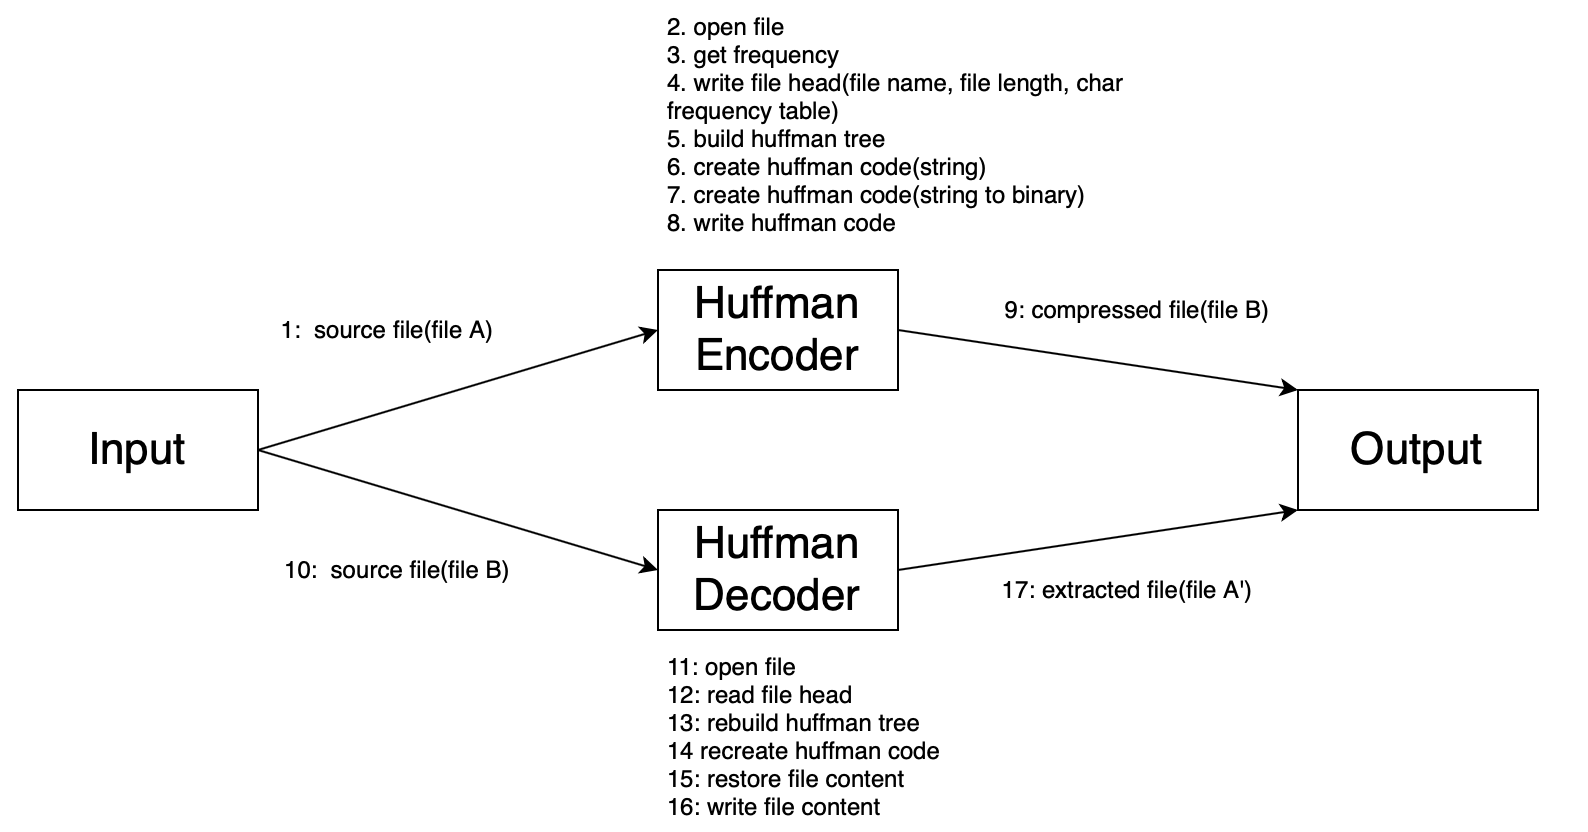
\includegraphics[scale=0.4]{/Users/_linxinhui_/Desktop/DSACurriculumDesign/CourseReport/pics/UML.png}
\caption{总体设计}
\end{figure}

\subsection{功能模块设计}\label{header-n93}

功能模块主要包括编码/压缩模块和解码/解压缩两大模块,其中包含了若干子模块, 如下粗体所示:

\textbf{编码模块:}

\begin{itemize}
\item
  打开文件, 扫描信源
\item
  统计每类字符出现的频度, \textbf{建立频度表}
\item
  根据频度表\textbf{创建Huffman树}
\item
  由Huffman树\textbf{生成Huffman码}(保存在码表中)
\item
  二次扫描信源, 根据码表编码, 将编码结果\textbf{字符串转换为位串}
\item
  写入编码/压缩文件并保存
\end{itemize}

\textbf{解码模块:}

\begin{itemize}
\item
  打开文件, 读取文件头(最重要的是频度表)
\item
  由频度表\textbf{重建Huffman树}
\item
  由Huffman树重新\textbf{生成Huffman码}(码表)
\item
  或通过Huffman树(\texttt{C版本}), 或通过反转码表(\texttt{Python版本})\textbf{反解出Huffman码}, 还原文件内容
\item
  写入文件, 完成解码/解压缩
\end{itemize}

(其实用户界面设计中也包含若干功能模块, 见下\texttt{用户界面设计}。)

所有功能模块的具体实现见下\texttt{各功能模块实现}。

\subsection{用户界面设计}\label{header-n123}

用C语言实现用户图形界面(非终端界面)困难而无用, Python则正好相反。这里用Python中的\texttt{tkinter}模块实现用户图形界面。

由于程序本身不具备很丰富的操作, 用户界面没有很复杂的层次, 只包括:

\begin{enumerate}
\def\labelenumi{\arabic{enumi}.}
\item
  主窗口, 用于提示用户程序的功能并给出功能对应的按钮控件供操作(C版本提示信息显示在终端中, 选择操作需要用户键入指令)
\item
  消息窗口, 用于提示用户确认操作、供用户选择待压缩/解压缩(下文简称操作)的文件(C版本中需要用户自行输入文件的绝对路径)、提示操作开始及提示操作结束
\item
  辅助窗口, 这个实质上是终端窗口, 在实际操作中内嵌在PyCharm中, 打印一系列调试信息到标准输出设备
\end{enumerate}

具体的用户图形界面不在这里展示了, 见下文\texttt{各功能模块实现}。

%—— 4 详细设计及系统实现

\section{详细设计及系统实现}\label{header-n134}

\subsection{存储结构设计}\label{header-n135}

为了(理论上)处理任何格式的编码, 以二进制的方式读文件(rb/read\_binary), 对读入的二进制位串(以下简称位串)以八位为处理单元处理。以八位为一个处理单元的原因是在很多语言中, 一个字符型变量占有的空间就是八位, 以C语言为例, 有:

{\setmainfont{Courier New Bold}              
\begin{lstlisting}
sizeof(char) == 8
\end{lstlisting}}

事实上这也是C语言中可以直接使用的占有位数(空间)最小的数据类型, Python语言中尽管没有字符的概念, 基本数据类型占有的空间往往也很大, 但我们仍然采用八位为处理单元处理原文件。正因为Python中没有字符的概念, 更没有\texttt{char}这种数据类型, 在Python源码我们严格地区分字符串与位串, 考虑到要对文件以二进制方式读写, 所谓'字符串'类型指的不是\texttt{str}而是\texttt{bytes}, 而位串本质上是二进制整数,  \texttt{int}型变量存储即可(这种机制引发了一个不大不小的问题, 到\texttt{各功能模块实现}部分再说, \texttt{bytes}与\texttt{int}类型的转换也留待后文说明)。

(在C代码中, 为了稳妥起见, 凡是严格的无符号类型都加上了unsigned前缀, 比如unsigned char, unsigned int, unsigned long以避免某些奇怪的错误。)

方便起见, 称一个八位位串为一个字符(本报告及源文件中的"字符"都应该理解为广义的八位位串, 这一点在说明抽象数据类型之前也提到过), 位串序列相同的称为一类, 如 00000000 和 11111111 是两个字符, 也是两类字符, 而 01010101 和 01010101是两个字符, 同时是一类字符。

一个八位位串最多可能有256种不同组合,意味着读入的文件(无论原来是何种格式, 读入后就是一个大型的二进制串)中最多有256种字符。

有了这些基础之后, 我们可以开始讨论存储结构设计, 先看\texttt{C版本}。

能用基本数据类型实现的结构不多说了, \texttt{C版本}中最重要的结构有两个:

\begin{enumerate}
\def\labelenumi{\arabic{enumi}.}
\item
  Huffman树
\item
  频度表
\end{enumerate}

先看Huffman树:

{\setmainfont{Courier New Bold}              
\begin{lstlisting}
/* Huffman树 */
typedef struct {
    unsigned char ch; /* 以8位为一个单元存储字符 */
    unsigned long freq; /* 字符频度(次数) */
    char *huf_code; /* 字符对应Huffman码 */
    int parent, lchild, rchild; /* 双亲和左右孩子 */
} HufTreeNode, *HufTree;
\end{lstlisting}}

要构建Huffman树, 首先定义树节点\texttt{HufTreeNode}, 每个树节点包括:

\begin{enumerate}
\def\labelenumi{\arabic{enumi}.}
\item
  字符(八位位串, 当然只关注叶节点的字符信息)
\item
  字符频度
\item
  字符对应的Huffman码, 在树中以字符串的形式存储, 写文件时转换成位串
\item
  树节点的双亲、左右孩子, 由于树用顺序表存储, 这三个指针退化为整数, 通过顺序表的位序找对应节点
\end{enumerate}

而Huffman树\texttt{HufTree}本质上是以\texttt{HufTreeNode}为元素的顺序表(即静态三叉表), 在已知字符数目(记\emph{char\_type\_num})的条件下可以知道Huffman树节点数量(记\emph{node\_num}), 有\emph{node\_num = 2 * char\_typenum - 1}, 从而通过:

{\setmainfont{Courier New Bold}              
\begin{lstlisting}
HufTree huf_tree = (HufTree)malloc(node_num * sizeof(HufTreeNode));
\end{lstlisting}}

即构造出了Huffman树的基本形态, 之后向其填充数据即可。

Huffman树本质上是一张顺序表, 频度表则是字典(其实说是顺序表也没有问题, 字典的说法更容易理解), 定义如下:

{\setmainfont{Courier New Bold}              
\begin{lstlisting}
/* 采用数组保存字符并统计字频, 以下定义存储字符频度的节点 */
typedef struct {
    /* 定义字符频度表及其对应元素(节点) */
    unsigned char ch; /* 以8位为一个单元存储字符 */
    unsigned long freq; /* 字符频度(次数) */
} CharFreqNode, *CharFreqTable;
\end{lstlisting}}

构建Huffman树首先要获取各类字符的频度, 存储字符频度至少可以采用两种结构:

\begin{enumerate}
\def\labelenumi{\arabic{enumi}.}
\item
  链表存储
\item
  顺序表(数组存储)
\end{enumerate}

其中, 链表这种结构的优点包括:

\begin{enumerate}
\def\labelenumi{\arabic{enumi}.}
\item
  动态地分配空间, 在数据规模变化较大的情况下可以显著地降低空间成本
\item
  对于增删节点一类的操作相当容易
\end{enumerate}

缺点则是, 链式结构作为一种随机存储结构, 并不便于查找某个特定节点, 这就意味着每读入一个字符就要扫描一遍链表, 时间成本太高。

考虑字符种类数最多不过256, 即使使用数组, 也未必造成多大的空间浪费, 使用数组下标匹配字符, 找一类指定字符根本不需要扫描整张表, 相对链表显然更有优势。

在某些情况(读入文件字符数较少)下, 未必出现256种字符, 在第一次扫描(统计字符频度后)对频度表排序, 去除字符频度为0的节点。

八位的位串最多能表示256中字符, 故定义:

{\setmainfont{Courier New Bold}              
\begin{lstlisting}
CharFreqTable table = (CharFreqTable)malloc(256 * sizeof(CharFreqNode));
\end{lstlisting}}

即得频度表。

\texttt{Python版本}在存储结构设计上则简单得多, 无论是列表还是字典, 都有原生的类型支持(\texttt{list}和\texttt{dict}):

{\setmainfont{Courier New Bold}              
\begin{lstlisting}
# 初始化变量
leaf_nodes_dict = {}  # 原数据-叶节点dict
char_freq_dict = {}  # 字符-频度dict
huf_code_dict = {}  # 叶节点-Huffman码dict
inverse_dict = {}  # 反转huf_code_dict中的键值对
huf_nodes = []  # Huffman树节点list
\end{lstlisting}}

这样就几乎完成了所有存储结构的定义, 其中\texttt{huf\_nodes}几乎就是日后的Huffman树, 其中元素的类型为\texttt{Node}, 是自定义类\texttt{Node}的实例, 关于\texttt{Node}类的定义, 见下\texttt{各功能模块实现}。

最后, 还有压缩文件的存储结构的设计。为了实现解码, 在压缩的过程中除了Huffman码外, 还需要在文件头写入若干信息, 于是压缩文件的结构为:

\begin{figure}[H]
\centering
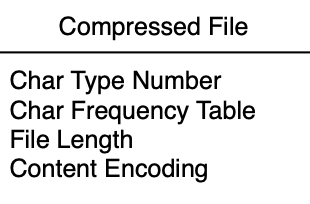
\includegraphics[scale=0.6]{../CourseReport/pics/compressed_file.png}
\caption{压缩文件存储结构}
\end{figure}

\subsection{核心算法设计}\label{header-n190}

核心算法大致有:

\begin{enumerate}
\def\labelenumi{\arabic{enumi}.}
\item
  构建Huffman树
\item
  编码
\item
  解码
\item
  字符串与位串的互化
\end{enumerate}

\textbf{构建Huffman树:}

使用Huffman算法构建Huffman树, Huffman算法是经典的贪心算法, 构造Huffman树的过程如下。

设待编码符号集中有n个符号, 对应n个权值(频度), 则构造出的哈夫曼树有n个叶子结点。设n个权值分别为w1, w2, ..., wn, 则哈夫曼树的构造规则为:

step1. 将w1, w2, ..., wn的集合视为包含n棵树的森林(每棵树只有一个根结点)

step2. 在森林中选出两个根结点的权值最小的树合并, 作为一棵新树的左、右子树, 且新树的根结点权值为其左、右子树根结点权值之和

step3. 从森林中删除选取的两棵树, 将新树加入森林

step4. 重复step2, step3, 直到森林中只剩一棵树, 该树即为所求得的哈夫曼树

Huffman树中所有的节点的度要么为0, 要么为1(国外的教材称这种树为满二叉树), 从而可以知道对一个有n个叶节点的Huffman树, 其节点数为2n - 1, 从而可以直接用循环的方法构造Huffman树(\texttt{C版本}),
当然倘若不知道上述关系, 也可以用递归的方式构造Huffman树(\texttt{Python版本})。

\textbf{生成Huffman码(编码):}

Huffman码的生成依赖于Huffman树, 要得到每个符号的代码, 从根节点遍历到每个叶节点, 为左分支指定0,
为右分支指定1即可得到Huffman码。

\textbf{解码:}

解码的一种最简单的方法是暴力搜索, 对码表求逆得反转码表(Huffman码-字符字典), 从解压文件中一次读入一位\texttt{0}或\texttt{1}, 暂存在某个变量(不妨称之为\texttt{data})中, 每读入一位, 就在反转码表中寻找\texttt{data}是否有对应的字符, 若有, 写入文件, 若无, 继续读入。这样做, 每读入一位都要遍历一遍码表, 虽然思路简单但效率极低。这种算法在\texttt{Python版本}中实现。

另一种显然更高效的思路是用Huffman树。给定Huffman树和一个位串, 解码的过程如下: 从根节点遍历到与某符号对应的叶节点, 就可以得到该节点的代码, 遍历路径上的每条分支都向码字贡献一个比特的数据(每条左分支贡献一个0, 每条右分支贡献一个1)。反之, 当知道码字时, 每次译码(一次翻译一个字符)都从根节点开始, 遇到\texttt{0}走左分支, 遇到\texttt{1}走右分支, 直到走到叶子节点, 重复该过程直到码字全部被译出。这种方式极大地提高了效率, 但是实现比较复杂, 在\texttt{C版本}中实现。

\textbf{字符串与位串的互化:}

上面生成Huffman码的算法生成的是字符串, 为了实现压缩, 写入文件时显然应该写入位串而非字符串。假设字符串内容存储在变量\texttt{string}中, 如\texttt{string\ ==\ "10100011"}, 位串存在变量\texttt{binary}中。

为方便写入文件, 尽管Huffman码是变长编码, 长度不定, 还是要设定以八位(一个字节)为处理单元, 每次处理八个长度单位的编码(这里的“八个长度”对字符串而言是八个字符, 对位串而言就是八位, 转化过程中字符串的一个字符与位串的一个位一一对应), 注意在文件末尾可能出现不足八个长度编码的问题, 要另外处理。

要处理位串, 显然要用到位运算, C和Python都提供了位运算供使用。具体地, 左移运算\texttt{\textless{}\textless{}}(在效果上)可以拓展位串的长度, 向位串的末尾加若干位, 按位与运算\texttt{\textbar{}}能够改变一位的值(具体地, 使\texttt{0}变为\texttt{1}), 而按位与运算\texttt{\&}能够"摘除"最高位的\texttt{1}(这个运算符只在\texttt{Python版本}中使用)。

\texttt{binary}在初始状态下是一个空串(等价于\texttt{0b0000000000}, 方便起见, 就理解为空), 每次操作时\texttt{binary}左移一位(相当于增加一位), 即\texttt{binary\ =\ binary\ \textless{}\textless{}\ 1}, 然后由从高位向低位的书顺序从\texttt{string}中读取一个字符, 倘若读入的字符是\texttt{0}, 不操作\texttt{binary}, 反之, 倘若读入的字符是\texttt{1}, 令\texttt{binary\ =\ binary\ \textbar{}\ 1}将当前为置为\texttt{1}。 重复这个过程直到整个文件编码完成。

上述过程写在一个循环里, 以八位为处理单元意味着每处理八个长度的编码就写入一次, 当然文件长度未必是八的整数倍, 最后大概率剩余不足八位的若干位, 此时只要调整循环控制变量的范围即可, 使用的算法与上述无异。

以上是对算法的描述, 不涉及语言层面的细节。在具体实现的过程, \texttt{C版本}和\texttt{Python版本}对互化过程的操作并不完全一样(尽管方法相同), 具体见下\texttt{各功能模块实现}。

\subsection{各功能模块实现}\label{header-n221}

下面开始介绍各功能模块的实现。在这个部分, 我先介绍\texttt{C版本}的实现, 再介绍\texttt{Python版本}的实现。先给出各个模块的代码(删去不必要的注释, 删去用于打印的语句, 删去用于分割的空行), 然后尽可能详细而简明地说明各个部分在干什么。

\subsubsection{C语言实现}\label{header-n223}

\texttt{C版本}struct的定义在\texttt{存储结构设计}部分已经讲过了, 这里从略。

其中最重要的两个函数就是\texttt{HuffmanEncoder}和\texttt{HuffmanDecoder}, 先看解码函数:

{\setmainfont{Courier New Bold}              
\begin{lstlisting}
int HuffmanEncoder(char *infile_name, char *outfile_name) {
    FILE *infile, *outfile;
    CharFreqTable table; /* 字符频度表, 统计节点频度并拷贝到树节点之后即被释放 */
    unsigned char temp_char; /* 暂存字符(8bits位串) */
    unsigned int char_type_num; /* 字符(8bits位串)种类数 */
    unsigned int file_len = 0; /* 文件长度 */
    unsigned int node_num; /* Huffman树中将会有的节点数, 由叶子节点数(字符数)确定 */
    HufTree huf_tree;
    char buffer[MAXCHARTYPE] = "\0"; /* 编码缓冲区 */
    unsigned int code_len;
    unsigned int i;

    if (GetFrequency(infile_name, &table, &char_type_num, &file_len) == ERROR) {
        return ERROR;
    }

    /* 若只有一种字符 */
    if (char_type_num == 1) {
        /* 打开文件 */
        outfile = fopen(outfile_name, "wb");
        if (outfile == NULL) {
            return ERROR;
        }

        /* 写入字符种类数、字符、字符频度 */
        fwrite((char *)(&char_type_num), sizeof(unsigned int), 1, outfile);
        fwrite((char *)(&table[0].ch), sizeof(unsigned char), 1, outfile);
        fwrite((char *)(&table[0].freq), sizeof(unsigned long), 1, outfile);

        free(table);

        fclose(outfile);
    }
    /* 若不止一种字符 */
    else {
        node_num = 2 * char_type_num - 1;

        huf_tree = (HufTree)malloc(node_num * sizeof(HufTreeNode));

        /* 初始化Huffman树的前char_type_num个节点 */
        for (i = 0; i < char_type_num; ++ i) {
            /* 将table的内容拷贝到树节点 */
            huf_tree[i].ch = table[i].ch;
            huf_tree[i].freq = table[i].freq;
            huf_tree[i].parent = 0;
        }

        /* 释放table */
        free(table);

        /* 初始化Huffman树的剩余节点 */
        for (i = char_type_num; i < node_num; ++ i) {
            huf_tree[i].parent = 0;
        }

        /* 构建Huffman树 */
        CreateHufTree(huf_tree, char_type_num, node_num);

        /* 生成Huffman码 */
        CreateHufCode(huf_tree, char_type_num);

        /* 开始写文件 */
        outfile = fopen(outfile_name, "wb");
        if (outfile == NULL) {
            return ERROR;
        }

        /* 向文件写入字符及其频度 */
        fwrite((char *)(&char_type_num), sizeof(unsigned int), 1, outfile);
        for (i = 0; i < char_type_num; ++ i) {
            fwrite((char *)(&huf_tree[i].ch), sizeof(unsigned char), 1, outfile);
            fwrite((char *)&huf_tree[i].freq, sizeof(unsigned long), 1, outfile);
        }

        /* 向文件写入文件长度 */
        fwrite((char *)(&file_len), sizeof(unsigned long), 1, outfile);

        /* 字符编码 */
        infile = fopen(infile_name, "rb");
        if (infile == NULL) {
            return ERROR;
        }
        fread((char *)(&temp_char), sizeof(unsigned char), 1, infile);
        while (!feof(infile)) {
            /* 匹配从infile读取的字符和存储在Huffman树中的字符, 并将对应Huffman码复制到buffer */
            for (i = 0; i < char_type_num; ++ i) {
                if (temp_char == huf_tree[i].ch) {
                    strcat(buffer, huf_tree[i].huf_code);
                }
            }

            /* 以8个长度(这里的长度既可以指bit, 也可指byte)为单元编码 */
            while (strlen(buffer) >= 8) {
                temp_char = '\0'; /* '\0'等价于0x00等价于00000000 */
                for (i = 0; i < 8; ++ i) {
                    temp_char <<= 1;
                    if (buffer[i] == '1') {
                        temp_char |= 1;
                    }
                }
                fwrite((char *)(&temp_char), sizeof(unsigned char), 1, outfile);
                strcpy(buffer, buffer + 8);
            }
            fread((char *)(&temp_char), sizeof(unsigned char), 1, infile);
        }
        
        /* 处理末尾buffer中(很有可能存在的)不足8个长度的编码 */
        code_len = strlen(buffer);
        if (code_len > 0) {
            temp_char = '\0';
            for (i = 0; i < code_len; ++ i) {
                temp_char = temp_char << 1;
                if (buffer[i] == '1') {
                    temp_char = temp_char | 1;
                }
            }
            temp_char <<= (8 - code_len);
            fwrite((char *)(&temp_char), sizeof(unsigned char), 1, outfile);
        }

        /* 关闭文件 */
        fclose(infile);
        fclose(outfile);

        /* 释放Huffman树占用的空间 */
        for (i = 0; i < char_type_num; ++ i) {
            free(huf_tree[i].huf_code);
        }
        free(huf_tree);
    }

    return OK;
}
\end{lstlisting}}

首先读文件并统计字符频次(这里增加了查验输入文件有效性的步骤), 使用\texttt{GetFrequency}函数完成:

{\setmainfont{Courier New Bold}              
\begin{lstlisting}
/* 读源文件, 统计词频, 存在table表中 */
if (GetFrequency(infile_name, &table, &char_type_num, &file_len) == ERROR) {
    return ERROR;
}
\end{lstlisting}}

\texttt{GetFrequency}函数的定义如下:

{\setmainfont{Courier New Bold}              
\begin{lstlisting}
int GetFrequency(char *infile_name, CharFreqTable *t, unsigned int *num, unsigned int *len) {
    FILE *infile;
    unsigned char temp_char; /* 暂存字符(8bits位串) */
    int i;

    /* 创建顺序表, 用8位存储字符, 最多能存256种字符, 数组/顺序表长度置为256 */
    *t = (CharFreqTable)malloc(MAXCHARTYPE * sizeof(CharFreqNode));
    if (*t == NULL) {
        printf("Space applying failed, please try again.");
        return FAILED;
    }

    /* 初始化暂存字符节点 */
    for (i = 0; i < 256; ++ i) {
        /* 数组的256个下标与(可能的)256个字符对应 */
        (*t)[i].ch = (unsigned char)i;
        (*t)[i].freq = 0;
    }

    /* 打开文件 */
    infile = fopen(infile_name, "rb");
    if (infile == NULL) {
        return ERROR;
    }

    /* 读文件, 获取字符频度 */
    fread((char *)(&temp_char), sizeof(unsigned char), 1, infile);
    while (!feof(infile)) {
        ++ (*t)[(int)temp_char].freq;
        ++ (*len);
        fread((char *)(&temp_char), sizeof(unsigned char), 1, infile);
    }

    /* 关闭文件 */
    fclose(infile);

    /* 对table按频度排序 */
    SortTable(t);

    /* 统计实际字符种类, 并剔除频度为0的字符 */
    for (i = 0; i < MAXCHARTYPE; ++ i) {
        if ((*t)[i].freq == 0) {
            break;
        }
    }
    (*num) = i;

    return OK;
}
\end{lstlisting}}

首先创建并初始化频度表(字符-频度字典), 创建使用\texttt{malloc}函数, 用八位存储字符, 最多能存256种字符, 表长度置为256:

{\setmainfont{Courier New Bold}              
\begin{lstlisting}
*t = (CharFreqTable)malloc(256 * sizeof(CharFreqNode));
\end{lstlisting}}

这256种字符事实上与0-255这256个整数对应, 故初始化频度表时键(字符)即为整数对应的无符号字符, 值(频度)均为0:

{\setmainfont{Courier New Bold}              
\begin{lstlisting}
for (i = 0; i < 256; ++ i) {
    (*t)[i].ch = (unsigned char)i;
    (*t)[i].freq = 0;
}
\end{lstlisting}}

开始第一次扫描文件, 打开关闭文件分别用\texttt{fopen}和\texttt{fclose}函数, 注意打开方式为\texttt{"rb"}(前面已经说明了原因)。读写文件分别使用\texttt{fread}和\texttt{fwrite}函数。读取文件内容的过程实际上是创建频度表的过程:

{\setmainfont{Courier New Bold}              
\begin{lstlisting}
fread((char *)(&temp_char), sizeof(unsigned char), 1, infile);
while (!feof(infile)) {
    ++ (*t)[(int)temp_char].freq;
    ++ (*len);
    fread((char *)(&temp_char), sizeof(unsigned char), 1, infile);
}
\end{lstlisting}}

至此, 频度获取完毕, 此时的频度表是无序的状态, 并且可能存在频度为0的节点, 我们先对频度表排序。

\texttt{SortTable}是一个辅助函数, 用于在获取字符频度之后对其排序, 这里使用的排序算法是冒泡排序:

{\setmainfont{Courier New Bold}              
\begin{lstlisting}
void SortTable(CharFreqTable *t) {
    int i, j;
    CharFreqNode temp;

    /* 按节点频度冒泡排序 */
    for (i = 0; i < MAXCHARTYPE - 1; ++ i) {
        for (j = i + 1; j < MAXCHARTYPE; ++ j) {
            if ((*t)[i].freq < (*t)[j].freq) {
                temp = (*t)[i];
                (*t)[i] = (*t)[j];
                (*t)[j] = temp;
            }
        }
    }

    return ;
}
\end{lstlisting}}

然后剔除频度为0的字符, 目的在于统计实际字符种类:

{\setmainfont{Courier New Bold}              
\begin{lstlisting}
for (i = 0; i < MAXCHARTYPE; ++ i) {
        if ((*t)[i].freq == 0) {
            break;
        }
    }
    (*num) = i;
\end{lstlisting}}

至此, 频度表构建完毕(且为有序状态), 顺便知道了原文件中字符的种类数, 字符种类数将被存在\texttt{char\_type\_num}中。

注意, 在字符种类数为1的情况下尽管可以构建Huffman树, 但由于建好的Huffman树中只有一个节点, 无法生成Huffman码, 考虑到程序健壮性(其实是功能完整性), 这里必须讨论只有一种字符的情况:

{\setmainfont{Courier New Bold}              
\begin{lstlisting}
/* 若只有一种字符 */
if (char_type_num == 1) {
    /* 打开文件 */
    outfile = fopen(outfile_name, "wb");
    if (outfile == NULL) {
        return ERROR;
    }

    /* 写入字符种类数、字符、字符频度 */
    fwrite((char *)(&char_type_num), sizeof(unsigned int), 1, outfile);
    fwrite((char *)(&table[0].ch), sizeof(unsigned char), 1, outfile);
    fwrite((char *)(&table[0].freq), sizeof(unsigned long), 1, outfile);

    free(table);

    fclose(outfile);
}
\end{lstlisting}}

当只有一种字符时, 不构建Huffman树, 不生成Huffman码, 只完成写文件头的操作, 依次写入字符种类数、唯一的一种字符及其频度。关闭文件,退出程序即可。注意C语言没有内存回收机制, 所以在退出程序前尽可能先销毁已经用过的诸如编码表、Huffman树一类的东西。

对于不止一种字符的情况, 同样要写文件头, 依次写入字符种类数、频度表(字符-频度字典)和文件长度(上面的情况不必写文件长度, 这里必须写):

{\setmainfont{Courier New Bold}              
\begin{lstlisting}
    outfile = fopen(outfile_name, "wb");
    if (outfile == NULL) {
        return ERROR;
    }

    fwrite((char *)(&char_type_num), sizeof(unsigned int), 1, outfile);
    for (i = 0; i < char_type_num; ++ i) {
        fwrite((char *)(&huf_tree[i].ch), sizeof(unsigned char), 1, outfile);
        fwrite((char *)&huf_tree[i].freq, sizeof(unsigned long), 1, outfile);
    }

    fwrite((char *)(&file_len), sizeof(unsigned long), 1, outfile);
\end{lstlisting}}

写完文件头, 开始构建Huffman树, 首先初始化。已知字符种类数, 实际上是知道了Huffman树中叶子节点的数量, 那么树中所有节点的数量满足:

{\setmainfont{Courier New Bold}              
\begin{lstlisting}
node_num = 2 * char_type_num - 1;
\end{lstlisting}}

从而:

{\setmainfont{Courier New Bold}              
\begin{lstlisting}
huf_tree = (HufTree)malloc(node_num * sizeof(HufTreeNode));
\end{lstlisting}}

于是初始化Huffman树中的所有节点:

{\setmainfont{Courier New Bold}              
\begin{lstlisting}
    /* 初始化Huffman树的前char_type_num个节点 */
    for (i = 0; i < char_type_num; ++ i) {
        /* 将table的内容拷贝到树节点 */
        huf_tree[i].ch = table[i].ch;
        huf_tree[i].freq = table[i].freq;
        huf_tree[i].parent = 0;
    }

    /* 初始化Huffman树的剩余节点 */
    for (i = char_type_num; i < node_num; ++ i) {
        huf_tree[i].parent = 0;
    }
\end{lstlisting}}

并构建Huffman树:

{\setmainfont{Courier New Bold}              
\begin{lstlisting}
int CreateHufTree(HufTree huf_tree, unsigned int char_type_num, unsigned int node_num) {
    unsigned int i;
    int minimum, second_minimum;

    for (i = char_type_num; i < node_num; ++ i) {
        SelectNode(huf_tree, i, &minimum, &second_minimum); /* 选取两个频次最小的节点 */
        huf_tree[i].lchild = minimum;
        huf_tree[i].rchild = second_minimum;
        huf_tree[i].freq = huf_tree[minimum].freq + huf_tree[second_minimum].freq;
        huf_tree[minimum].parent = i;
        huf_tree[second_minimum].parent = i;
    }

    return OK;
}
\end{lstlisting}}

构造Huffman树的算法在\texttt{核心算法设计}部分已经说清楚了, 借助静态三叉表, 构造的过程并不复杂。

构建Huffman树需要从森林中找到两个权值最小的(根)节点, 这一功能由\texttt{SelectNode}函数完成:

{\setmainfont{Courier New Bold}              
\begin{lstlisting}
int SelectNode(HufTree huf_tree, unsigned int n, int *minimum, int *second_minimum) {
    unsigned int i;
    unsigned long min;

    /* 找最小节点 */
    min = ULONG_MAX; /* ULONG_MAX是unsigned long int的十进制最大值 */
    for (i = 0; i < n; ++ i) {
        if (huf_tree[i].parent == 0 && huf_tree[i].freq < min) {
            min = huf_tree[i].freq;
            *minimum = i;
        }
    }
    huf_tree[*minimum].parent = CHOSEN;

    /* 找次小节点 */
    min = ULONG_MAX;
    for (i = 0; i < n; ++ i) {
        if (huf_tree[i].parent == 0 && huf_tree[i].freq < min) {
            min = huf_tree[i].freq;
            *second_minimum = i;
        }
    }

    return OK;
}
\end{lstlisting}}

这里用到的\texttt{ULONG\_MAX}是unsigned long int的十进制最大值, 由\texttt{limit.h}提供。遍历两次找到Huffman树表中权值最小和次小的节点, 返回其位序, 注意在找完最小节点后, 加上以下操作:

{\setmainfont{Courier New Bold}              
\begin{lstlisting}
huf_tree[*minimum].parent = CHOSEN;
\end{lstlisting}}

\texttt{CHOSEN}是一个任意的非零值, 这句的目的在于把最小节点标记出来, 避免在找次小节点时产生影响。

至此, 构建Huffman树完成, Huffman树存在一张静态三叉表中, 设表长为2n - 1, 则前n个元素对应的都是Huffman树的叶节点, 最后一个元素一定是Huffman树的根节点, 这一点是未来完成对某些特殊节点操作的重要依据。

继续, 生成Huffman码:

{\setmainfont{Courier New Bold}              
\begin{lstlisting}
int CreateHufCode(HufTree huf_tree, unsigned int char_type_num) {
    unsigned int i;
    int cur, parent;
    int index;
    char *temp_code = NULL;

    temp_code = (char *)malloc(MAXCHARTYPE * sizeof(char));
    temp_code[MAXCHARTYPE - 1] = '\0';

    for (i = 0; i < char_type_num; ++ i) {
        index = MAXCHARTYPE - 1;
        cur = i;
        parent = huf_tree[cur].parent;

        /* 从叶子节点到根节点, 反向生成Huffman码 */
        while (parent != 0) {
            if (huf_tree[parent].lchild == cur) {
                /* 左分支编'0' */
                index -= 1;
                temp_code[index] = '0';
            }
            else {
                /* 左分支编'1' */
                index -= 1;
                temp_code[index] = '1';
            }

            cur = parent;
            parent = huf_tree[cur].parent;
        }

        /* 将生成的编码保存到树节点 */
        huf_tree[i].huf_code = (char *)malloc((MAXCHARTYPE - index) * sizeof(char));
        strcpy(huf_tree[i].huf_code, &temp_code[index]); /* 正向保存Huffman码 */
    }

    free(temp_code);

    return OK;
}
\end{lstlisting}}

生成的Huffman码最终存在树节点中, 在此之前(构造的过程中), 使用一个临时变量\texttt{temp\_code}暂存Huffman码。\texttt{temp\_code}的长度不定, 指定一个足够大的数即可。从叶节点(如何判定叶节点,
上面给了一个简单的方法)出发, 依次判定当前节点\texttt{cur}是其双亲节点\texttt{parent}的左孩子还是右孩子, 从而确定向\texttt{temp\_char}中添加\texttt{0}或\texttt{1}, 用\texttt{index}指示当前编码的位置在\texttt{temp\_char}中的位置(显然, 每加入一位, index自减1)。为一个叶子节点编码完成后, 将\texttt{temp\_code}的内容复制到树节点即可。简单地说, 生成Huffman的过程是逆向生成, 正向保存。重复该过程知道所有叶子节点编码完毕, Huffman码生成完毕。

最后, 根据码表(字符-Huffman码字典)对原文件编码:

{\setmainfont{Courier New Bold}              
\begin{lstlisting}
    /* 字符编码 */
    infile = fopen(infile_name, "rb");
    if (infile == NULL) {
        return ERROR;
    }
    fread((char *)(&temp_char), sizeof(unsigned char), 1, infile);
    while (!feof(infile)) {
        /* 匹配从infile读取的字符和存储在Huffman树中的字符, 并将对应Huffman码复制到buffer */
        for (i = 0; i < char_type_num; ++ i) {
            if (temp_char == huf_tree[i].ch) {
                strcat(buffer, huf_tree[i].huf_code);
            }
        }

        /* 以8个长度(这里的长度既可以指bit, 也可指byte)为单元编码 */
        while (strlen(buffer) >= 8) {
            temp_char = '\0'; /* '\0'等价于(0x00)_16等价于(00000000)_2 */
            for (i = 0; i < 8; ++ i) {
                temp_char <<= 1;
                if (buffer[i] == '1') {
                    temp_char |= 1;
                }
            }
            fwrite((char *)(&temp_char), sizeof(unsigned char), 1, outfile);
            strcpy(buffer, buffer + 8);
        }
        fread((char *)(&temp_char), sizeof(unsigned char), 1, infile);
    }
        
    /* 处理末尾buffer中(很有可能存在的)不足8个长度的编码 */
    code_len = strlen(buffer);
    if (code_len > 0) {
        temp_char = '\0';
        for (i = 0; i < code_len; ++ i) {
            temp_char = temp_char << 1;
            if (buffer[i] == '1') {
                temp_char = temp_char | 1;
            }
        }
        temp_char <<= (8 - code_len);
        fwrite((char *)(&temp_char), sizeof(unsigned char), 1, outfile);
    }
\end{lstlisting}}

编码过程是实现字符串转位串的过程。二次扫描原文件, 每次读入一个字节的数据, 实际就是读入一个字符并存储在\texttt{temp\_char}中, 在Huffman树中找到这个字符, 更重要的是找到这个字符对应的Huffman码。在处理Huffman码时, 仍以八位为处理单元(\texttt{Python版本}同理), 但找到的字符的编码长度未必固定,
这是需要引入一个简易缓冲区(简易到只是一个字符数组)\texttt{buffer}。每次读取一个字符的Huffman码存入\texttt{buffer}, 当\texttt{buffer}的长度大于八的时候转码(字符串转位串), 每次处理八位并写入文件。转码的过程在\texttt{核心算法设计}已经讲过, 首先构造空串, 通过左移操作增加位, 通过按位或操作更新一位(当然更新与否取决于字符串的情况)。字符串从高位向低位读, 位串从低位向高位延伸。当然文件末尾可能有不足八位的位串需要单独处理, 处理的方式与上述过程一致, 区别仅在于处理的次数不同而已。

编码完成, 关闭文件, 释放Huffman树占用的空间, 至此, 编码完成, 压缩文件已生成。

以压缩文件作为input, 解压过程由\texttt{HuffmanDecoder}函数完成:

{\setmainfont{Courier New Bold}              
\begin{lstlisting}
int HuffmanDecoder(char *infile_name, char *outfile_name) {
    FILE *infile, *outfile;
    HufTree huf_tree;
    unsigned int root; /* 根节点地址 */
    unsigned int char_type_num;
    unsigned int node_num;
    unsigned char temp_char; /* 暂存8bits编码 */
    unsigned long file_len = 0;
    unsigned long writen_len = 0;
    unsigned int i;

    /* 打开文件 */
    infile = fopen(infile_name, "rb");
    if (infile == NULL) {
        return ERROR;
    }

    /* 读取文件头信息(字符数) */
    fread((char *)(&char_type_num), sizeof(unsigned int), 1, infile);

    /* 解码, 当只有一种字符时 */
    if (char_type_num == 1) {
        /* 读文件头信息(字符, 文件长度) */
        fread((char *)(&temp_char), sizeof(unsigned char), 1, infile);
        fread((char *)(&file_len), sizeof(unsigned int), 1, infile);

        /* 解码 */
        outfile = fopen(outfile_name, "wb");
        if (outfile == NULL) {
            return ERROR;
        }
        while (file_len > 0) {
            fwrite((char *)(&temp_char), sizeof(unsigned char), 1, outfile);
            -- file_len;
        }

        /* 关闭文件 */
        fclose(infile);
        fclose(outfile);
    }
    /* 解码, 当不止一种字符时 */
    else {
        node_num = 2 * char_type_num - 1;
        
        huf_tree = (HufTree)malloc(node_num * sizeof(HufTreeNode));

        /* 初始化Huffman树 */
        for (i = 0; i < char_type_num; ++ i) {
            fread((char *)(&huf_tree[i].ch), sizeof(unsigned char), 1, infile);
            fread((char *)(&huf_tree[i].freq), sizeof(unsigned long), 1, infile);
            huf_tree[i].parent = 0;
        }
        for (i = char_type_num; i < node_num; ++ i) {
            huf_tree[i].parent = 0;
        }

        /* 重建Huffman树 */
        CreateHufTree(huf_tree, char_type_num, node_num);

        /* 解码 */
        fread((char *)(&file_len), sizeof(unsigned long), 1, infile);
        outfile = fopen(outfile_name, "wb");
        if (outfile == NULL) {
            return ERROR;
        }
        root = node_num - 1;
        while (TRUE) {
            /* 以 8bits 为一个处理单元 */
            fread((char *)(&temp_char), sizeof(unsigned char), 1, infile);
            for (i = 0; i < 8; ++ i) {
                if ((temp_char & 128) == 0) {
                    root = huf_tree[root].lchild;
                }
                else {
                    root = huf_tree[root].rchild;
                }
                if (root < char_type_num) {
                    fwrite((char *)(&huf_tree[root].ch), sizeof(unsigned char), 1, outfile);
                    ++ writen_len;
                    if (writen_len == file_len) {
                        break;
                    }
                    root = node_num - 1;
                }
                temp_char <<= 1;
            }
            if (writen_len == file_len) {
                break;
            }
        }

        /* 关闭文件 */
        fclose(infile);
        fclose(outfile);

        /* 释放Huffman树占用的空间 */
        free(huf_tree);
    }

    return OK;
}
\end{lstlisting}}

首先打开文件读文件, 这里首先要考虑的是文件中的字符种类数, 若只有一种字符, 不必建树:

{\setmainfont{Courier New Bold}              
\begin{lstlisting}
/* 解码, 当只有一种字符时 */
if (char_type_num == 1) {
    /* 读文件头信息(字符, 文件长度) */
    fread((char *)(&temp_char), sizeof(unsigned char), 1, infile);
    fread((char *)(&file_len), sizeof(unsigned int), 1, infile);

    /* 解码 */
    outfile = fopen(outfile_name, "wb");
    if (outfile == NULL) {
        return ERROR;
    }
    while (file_len > 0) {
    	fwrite((char *)(&temp_char), sizeof(unsigned char), 1, outfile);
        -- file_len;
    }

    /* 关闭文件 */
    fclose(infile);
    fclose(outfile);
}
\end{lstlisting}}

若不止一种字符, 这里借助Huffman树解码(\texttt{Python版本}使用反转码表, 相比之下\texttt{C版本}的方法先进得多), 使用\texttt{CreateHufTree}重建Huffman树, 过程与上面编码过程中的一致, 不多说了。看解码过程:

{\setmainfont{Courier New Bold}              
\begin{lstlisting}
/* 解码 */
fread((char *)(&file_len), sizeof(unsigned long), 1, infile);
outfile = fopen(outfile_name, "wb");
if (outfile == NULL) {
    return ERROR;
}
root = node_num - 1;
while (TRUE) {
    /* 以 8bits 为一个处理单元 */
    fread((char *)(&temp_char), sizeof(unsigned char), 1, infile);
    for (i = 0; i < 8; ++ i) {
    if ((temp_char & 128) == 0) {
        root = huf_tree[root].lchild;
    }
    else {
    root = huf_tree[root].rchild;
    }
    if (root < char_type_num) {
    fwrite((char *)(&huf_tree[root].ch), sizeof(unsigned char), 1, outfile);
    ++ writen_len;
        if (writen_len == file_len) {
            break;
        }
    root = node_num - 1;
    }
    temp_char <<= 1;
    }
    if (writen_len == file_len) {
        break;
    }
}
\end{lstlisting}}

在说明解码算法之前, 首先要再强调一遍Huffman树结构: Huffman树用静态三叉表存储, 其长度为2n-1, 前n个节点是叶子节点, 最后一个节点是Huffman树的根节点。

这里借助Huffman树解码, 解码的过程实质上是通过读入的二进制序列找到一条从根节点到叶子节点的路径,
并读出路径终点(叶节点)存着的字符并写入文件。

注意我们读入时以八位(一个字节)为一个处理单元, 并且是从高位向低位处理, 为了得到最高位一位的数据,
需要将读入的一个字节的数据与\texttt{128}做与运算(128等价于0b10000000, 与运算的结果视最高位为\texttt{1}或\texttt{0}而为\texttt{1}或\texttt{0})得到当前位的信息, 根据其值决定由左分支往下走还是由右分支往下走:

{\setmainfont{Courier New Bold}              
\begin{lstlisting}
if ((temp_char & 128) == 0) {
    root = huf_tree[root].lchild;
}
else {
    root = huf_tree[root].rchild;
}
\end{lstlisting}}

这样就处理完了一位。每次处理完一位, 都要判断当前是否走到了叶节点, 更直接地说, 是否找到了与当前编码对应的字符, 若是, 将找到的字符写入文件(写入文件后读取新的位前要回到树的根节点), 否则什么也不做, 继续向当前编码中增加位:

{\setmainfont{Courier New Bold}              
\begin{lstlisting}
if (root < char_type_num) {
    fwrite((char *)(&huf_tree[root].ch), sizeof(unsigned char), 1, outfile);
    ++ writen_len;
    root = node_num - 1;
}
\end{lstlisting}}

注意写完文件后要判断是否到达文件尾, 换言之, 是否还有新的位需要继续处理:

{\setmainfont{Courier New Bold}              
\begin{lstlisting}
if (writen_len == file_len) {
    break;
}
\end{lstlisting}}

重复上述过程直到还原出原文件。最后关闭文件并释放Huffman树占用的空间完成解压。

至此, 编码器和解码器的实现说明完毕, 下面是关于交互方式的说明。

\texttt{OutputInfo}函数实现交互信息, 其功能为用\texttt{printf}函数打印若干信息, 提示用户进行相关操作, 如下:

{\setmainfont{Courier New Bold}              
\begin{lstlisting}
void OutputInfo() {
    /* 清屏, macOS/Linux下使用system("clear"); */
    system("cls");

    /* 简单交互 */
    printf("-------Huffman En-Decoder-------\n");
    printf("@author: _linxinhui_\n");
    /* Other Info:
    printf("@class: CS1901\n");
    printf("@No: 120191080104\n"); */
    printf("@version: 0.1\n\n");
    printf("Operations are as follows:\n1. To Compress\n2. To Extract\n3. To Quit\n");
    printf("Please choose an operation(enter the number): ");

    return ;
}
\end{lstlisting}}

在主函数中调用\texttt{OutputInfo}打印交互信息, 通过用户输入选择操作(对于输入错误的情况也可以给出错误提示并重新开始)并在操作完成后提示操作成功:

{\setmainfont{Courier New Bold}              
\begin{lstlisting}
int main() {
    char infile_name[256], outfile_name[256]; /* 输入输出文件名 */
    int option, flag; /* option选择操作, flag判定En/Decode状态 */
    char ch[2]; /* 用gets(ch)达到getchar()等待键盘输入的效果 */
    
    while (TRUE) {
        flag = 0;
    /* 选择操作 */
    LOOP:
        OutputInfo();
        fflush(stdin); /* 清空标准输入缓冲区, 下同从略 */
        scanf("%d", &option);

        if (option == 3) {
            /* 直接退出 */
            printf("The program has run to completion.\n");
            printf("Thanks for using this program!\n");
            break;
        }
        else if (option == 1 || option == 2) {
            /* 读取输入输出文件的(绝对)路径 */
            printf("Please enter the absolute path of the input file:\n");
            fflush(stdin);
            gets(infile_name);
            printf("Please enter the absolute path of the output file:\n");
            fflush(stdin);
            gets(outfile_name);
        }
        else {
            /* 输入错误 */
            printf("The selected function does not exist, please try again!\n");
            printf("Press any key to continue...\n");
            fflush(stdin);
            gets(ch);
            goto LOOP;
        }

        /* 选择操作 */
        switch (option) {
            case 1:
                printf("Checking input validity, please wait......\n");
                flag = HuffmanEncoder(infile_name, outfile_name);
                if (flag == ERROR) {
                    printf("Error(file not found), please try again!\n");
                    printf("Press any key to continue...");
                    fflush(stdin);
                    gets(ch);
                    goto LOOP;
                }
                printf("Compressing, please wait......\n");
                break;
            case 2:
                printf("Checking input validity, please wait......\n");
                flag = HuffmanDecoder(infile_name, outfile_name);
                if (flag == ERROR) {
                    printf("Error(file not found), please try again!\n");
                    printf("Press any key to continue...");
                    fflush(stdin);
                    gets(ch);
                    goto LOOP;
                }
                printf("Extracting, please wait......\n");
                break;
        }

        printf("Operation completed!\n");
    }

    system("pause");
    return 0;
}
\end{lstlisting}}

\subsubsection{Python语言实现}\label{header-n290}

{\setmainfont{Courier New Bold}              
\begin{lstlisting}
class Node(object):

    def __init__(self, value=None, lchild=None, rchild=None, parent=None):
        self.value = value
        self.lchild = lchild
        self.rchild = rchild
        self.parent = parent

    def build_parent_node(lchild, rchild):
        node = Node(value=lchild.value+rchild.value, lchild=lchild, rchild=rchild)
        lchild.parent = node
        rchild.parent = node
        return node

    def encode_node(node):
        if node.parent == None:
            return b''
        if node.parent.lchild == node:
            return Node.encode_node(node.parent) + b'0'
        else:
            return Node.encode_node(node.parent) + b'1'
\end{lstlisting}}

这里定义了一个Huffman树节点类, 将单个节点定义为一个类可以极大地简化操作。

Node类中包含三个方法, \texttt{init}是一个对象方法, 注意self参数。

\texttt{build\_parent\_node}方法接收两个(叶子)节点, 新建一个节点作为这两个节点的parent, 生成并返回二叉树。
\texttt{encode\_node}方法接收一个\texttt{Node}对象(也是叶子节点)作为参数, 采用递归的方式求该节点的Huffman码, 当node\_parent == None时, 意味着找到了从叶子节点到根节点的通路, 递归结束, 当递归还在进行时则判定node是node\_parent的左孩子/右孩子并对应地在传入的叶节点的Huffman码中写入'0'或'1'(写入的是一个\texttt{bytes}类型的字符串)。

\texttt{build\_parent\_node}方法在下面\texttt{build\_huffman\_tree}函数中用到, \texttt{encode\_node}方法在下面\texttt{create\_huffman\_code}函数中用到。

注意这里的\texttt{encode\_node}方法是用递归的方式定义的, 下面构建Huffman树的函数同样是用递归的方式定义的, Python语言对递归深度有限制:

{\setmainfont{Courier New Bold}              
\begin{lstlisting}
>>> import sys
>>> sys.getrecursionlimit()
1000
\end{lstlisting}}

当前系统的默认值为1000, 压缩大文件时可能引发RuntimeError: maximum recursion depth exceeded, 故需要调整调整最大递归深度, 这里设置为1000000:

{\setmainfont{Courier New Bold}              
\begin{lstlisting}
sys.setrecursionlimit(1000000)
\end{lstlisting}}

实现Huffman编解码器, 核心函数有二(\texttt{huffman\_encoder()}\\和\texttt{huffman\_decoder()}), 先看编码函数:

{\setmainfont{Courier New Bold}              
\begin{lstlisting}
def huffman_encoder(infile_name):
    bytes_width = 1
    huf_nodes = []
    infile = open(infile_name, 'rb')
    infile.seek(0, 2)
    file_len = infile.tell() / bytes_width
    infile.seek(0)
    i = 0
    buffer = [b''] * int(file_len)
    while i < file_len:
        buffer[i] = infile.read(bytes_width)
        if char_freq_dict.get(buffer[i], -1) == -1:
            char_freq_dict[buffer[i]] = 0
        char_freq_dict[buffer[i]] += 1
        i = i + 1
    infile.close()
    for elem in char_freq_dict.keys():
        leaf_nodes_dict[elem] = Node(char_freq_dict[elem])
        huf_nodes.append(leaf_nodes_dict[elem])
    create_huffman_code(True)
    head = sorted(char_freq_dict.items(), key = lambda x: x[1], reverse = True)
    bit_width = 1
    if head[0][1] > 16777215:
        bit_width = 4
    elif head[0][1] > 65535:
        bit_width = 3
    elif head[0][1] > 255:
        bit_width = 2
    outfile_name = infile_name.split('.')
    outfile_name = outfile_name[0] + '.hufzip'
    outfile = open(outfile_name, 'wb')
    outfile_name = infile_name.split('/')
    outfile.write((outfile_name[len(outfile_name) - 1] + '\n').encode(encoding = 'utf-8'))
    outfile.write(int.to_bytes(len(huf_code_dict), 2, byteorder = 'big'))
    outfile.write(int.to_bytes(bit_width, 1, byteorder = 'big'))
    for elem in huf_code_dict.keys():
        outfile.write(elem)
        outfile.write(int.to_bytes(char_freq_dict[elem], bit_width, byteorder = 'big'))
    i = 0
    raw = 0b1
    while i < file_len:
        for elem in huf_code_dict[buffer[i]]:
            raw = raw << 1
            if elem == 49:
                raw = raw | 1
            if raw.bit_length() == 9:
                raw = raw & (~(1 << 8))
                outfile.write(int.to_bytes(raw, 1, byteorder = 'big'))
                outfile.flush()
                raw = 0b1
        i = i + 1
    if raw.bit_length() > 1:
        raw = raw << (8 - (raw.bit_length() - 1))
        raw = raw & (~(1 << raw.bit_length() - 1))
        outfile.write(int.to_bytes(raw, 1, byteorder = 'big'))
    outfile.close()
\end{lstlisting}}

\texttt{huffman\_encoder}函数实现了Huffman编码, 它包含三个主要步骤:

\begin{enumerate}
\def\labelenumi{\arabic{enumi}.}
\item
  读文件, 构造字符-频度表
\item
  构建Huffman树, 生成Huffman码
\item
  编码, 写文件
\end{enumerate}

(在\texttt{1}的读文件步骤中, 文件内容已经被保存在buffer这个list中, 故在编码过程中无需再次读取文件内容。)

{\setmainfont{Courier New Bold}              
\begin{lstlisting}
# 文件预处理
bytes_width = 1
infile = open(infile_name, 'rb')
infile.seek(0, 2)
file_len = infile.tell() / bytes_width
print("\nfile length: %d" % file_len)
infile.seek(0)
\end{lstlisting}}

\texttt{bytes\_width}是每次读取的字符宽度(以字节为单位), 文件预处理步骤打开文件并读取了文件长度, 保存在\texttt{file\_len}中, 具体地, \texttt{open(name{[},\ mode{[},\ buffering{]}{]})}打开文件, \texttt{fileObject.seek(offset{[},\ whence{]})}移动文件指针, 先移动到文件尾, 通过\texttt{tell()}方法返回文件的当前位置, 即文件指针当前位置(相对于文件头), 即文件长度\texttt{file\_len}, 最后把文件指针移动到文件头以继续操作。

{\setmainfont{Courier New Bold}              
\begin{lstlisting}
# 建立频度(权值)表
i = 0
buffer = [b''] * file_len
while i < file_len:
    buffer[i] = infile.read(bytes_width)
    if char_freq_dict.get(buffer[i], -1) == -1:
        char_freq_dict[buffer[i]] = 0
    char_freq_dict[buffer[i]] += 1
    i = i + 1
\end{lstlisting}}

和\texttt{version0.2}中的一样, 以\texttt{rb}方式打开文件后每次读取八位(一个字节)的位串作为一个字节。

读取文件内容, 使用\texttt{fileObject.read(size)}从文件每次读取一个texttt{bytes\_width}(一个字节)的数据,
暂存在\texttt{buffer}中, 继而统计词频, 保存在texttt{char\_freq\_dict}中(这里使用\texttt{dict.get(key,\ default\ =\ None)}判定当前读到的字符是否已经存在于texttt{char\_freq\_dict}里, 若不存在则存入后进行下一步操作),\ 进行到这一步, 文件内容已经全部保存至texttt{buffer}, 可以关闭文件:

{\setmainfont{Courier New Bold}              
\begin{lstlisting}
infile.close()
\end{lstlisting}}

至此, 字符频度表构建完毕(注意还是无序的状态), 输出频度表测试不多说了, 下面开始构建Huffman树, 并生成Huffman码。

{\setmainfont{Courier New Bold}              
\begin{lstlisting}
huf_nodes = []  # 节点列表, 用于构建Huffman树

# 将频度表拷贝至叶子节点
for elem in char_freq_dict.keys():
    leaf_nodes_dict[elem] = Node(char_freq_dict[elem])
    huf_nodes.append(leaf_nodes_dict[elem])

# 构建Huffman树
huf_tree = build_huffman_tree(huf_nodes)

# 生成Huffman码
create_huffman_code(False)
\end{lstlisting}}

创建叶子节点, 将叶子节点拷贝到texttt{huh\_nodes}后就开始创建Huffman树并生成Huffman码,
texttt{build\_huffman\_tree}和texttt{create\_huffman\_code}函数如下:

{\setmainfont{Courier New Bold}              
\begin{lstlisting}
def build_huffman_tree(li):
    if len(li) == 1:
        return li
    sorted_li = sorted(li, key = lambda x: x.value, reverse = False)
    parent = Node.build_parent_node(sorted_li[0], sorted_li[1])
    sorted_li.pop(0)
    sorted_li.pop(0)
    sorted_li.append(parent)
    return build_huffman_tree(sorted_li)
\end{lstlisting}}

\texttt{build\_huffman\_tree}接收一个\texttt{list}作为参数, 该\texttt{list}将存放Huffman树。

\texttt{build\_huffman\_tree()}采用递归的方式构造Huffman树, 递归出口为\texttt{len(list)\ ==\ 1}, 即树中只有一个(根)节点, 也即传入的\texttt{list}从存放森林转变为存放(二叉)树。

构造Huffman树, 首先对传入的\texttt{list}中所有树节点按权值(频次)排序, 这里使用\texttt{sorted()}函数,
其原型为\texttt{sorted(iterable,\ key\ =\ None,\ reverse\ =\ False)}, 其中\texttt{iterable}可以是任意可迭代对象(这里为列表), \texttt{key}给出了排序的依据(这里构造了一个匿名函数, 设置排序依据为列表中Node对象的权值), 最后的\texttt{reverse}参数决定升序/降序排列(这里按降序排列)。

排序的结果是频度最小的两个节点被放在了列表开头, 选取这两个节点作为参数, 调用\texttt{build\_parent\_node}方法构建Huffman树的子树, 然后将这两个节点从列表中删除, 并将新生成的树的根节点加入列表, 重复上述过程直到Huffman树构建完毕。

{\setmainfont{Courier New Bold}              
\begin{lstlisting}
def create_huffman_code(flag):
    for elem in leaf_nodes_dict.keys():
        huf_code_dict[elem] = Node.encode_node(leaf_nodes_dict[elem])
\end{lstlisting}}

得益于Node类的引入, 生成Huffman编码的过程非常简单, 对叶子节点使用\texttt{encode\_node()}方法即可。

这里传入的\texttt{flag}决定了是否输出码表供测试, 本质就是打印一个字典, 不是重要内容, 从略。

\texttt{3}的写文件步骤是压缩过程中最关键的步骤。

写文件首先写文件头信息(压缩文件头部包含的信息), 文件头信息中包含:

\begin{itemize}
\item
  文件名
\item
  构建的Huffman树中节点的数量
\item
  编码表宽度
\item
  编码表
\end{itemize}

这些信息保存在压缩文件中, 在解压过程被读出供还原原文件。

{\setmainfont{Courier New Bold}              
\begin{lstlisting}
# 动态选择编码表宽度(优化文件头)
head = sorted(char_freq_dict.items(), key = lambda x: x[1], reverse = True)
# head[0][1]即是文件中出现次数最多的字符出现的次数
bit_width = 1
if head[0][1] > 16777215: # 16777215 == 2e24 - 1
    bit_width = 4
elif head[0][1] > 65535: # 65535 == 2e16 - 1
    bit_width = 3
elif head[0][1] > 255: # 255 == 2e8 - 1
    bit_width = 2
\end{lstlisting}}

这一段的作用如注释, 在于动态选择编码表的宽度, 编码表是由(key, value)这样的键值对组成的表, 其中\texttt{key}的长度是固定的(一个字节), 但\texttt{value}的值可大可小, 这里通过其最大值确定\texttt{value}的上界, 再通过该上界确定编码表的宽度(具体见下), 这里设置了三个阈值, 分别是\texttt{2e8\ -\ 1}, \texttt{2e16\ -\ 1}, \texttt{2e24\ -\ 1}。

\texttt{sorted()}函数的说明见上, 这里还使用了\texttt{fileObject.items()}, 其功能为返回包含若干(key,
value)形式的元组的\texttt{dict\_items}对象, 这一对象而后在\texttt{sorted()}函数中依据匿名函数\texttt{lambda\ x:\ x{[}1{]}}降序排序, 更准确的说, 这一步将\texttt{char\_freq\_dict}中的所有键值对取出,
根据值的大小逆序排列, 最后的排列结果存在head这一列表中, 此时head的元素是形如(key, value)的元组, 访问key或value需要两次引用。

读取\texttt{head{[}0{]}{[}1{]}}, 也即读取编码表中出现频次最高的字符的频次, 根据该频次的大小动态调整编码表的字节长度, 优化文件头大小。

{\setmainfont{Courier New Bold}              
\begin{lstlisting}
# 写入文件头(文件信息)
outfile_name = infile_name.split('.')
outfile_name = outfile_name[0] + '.hufzip'
outfile = open(outfile_name, 'wb')
outfile_name = infile_name.split('/')
outfile.write((outfile_name[len(outfile_name) - 1] + '\n').encode(encoding = 'utf-8'))
outfile.write(int.to_bytes(len(huf_code_dict), 2, byteorder = 'big'))
outfile.write(int.to_bytes(bit_width, 1, byteorder = 'big'))
# 写入文件头(编码表)
for elem in huf_code_dict.keys():
    outfile.write(elem)
    outfile.write(int.to_bytes(char_freq_dict[elem], bit_width, byteorder = 'big'))
\end{lstlisting}}

写文件使用\texttt{fileObject.write({[}str{]})}, \texttt{write()}方法用于向文件中写入指定字符串, 若文件打开模式带有\texttt{\textquotesingle{}b\textquotesingle{}}, 那么写入内容时, \texttt{str}要用\texttt{encode()}方法转为\texttt{bytes}。

压缩文件的文件名(基本名)与源文件相同, 拓展名为\texttt{.hufzip}, \texttt{huffman\_encoder()}读入文件的绝对路径, 从中读取出文件名需要使用\texttt{,\ split()}方法进行切片操作, 其原型为\texttt{str.split(str\ =\ "",\ num\ =\ string.count(str))}。

依次写入文件名、Huffman树节点数量、编码表宽度和编码表, 写入过程中涉及整数(准确地说是十进制正整数)与\texttt{bytes}类型的转化, 这使用\texttt{to\_bytes()函数}, 在\texttt{Python交互模式}下键入:

{\setmainfont{Courier New Bold}              
\begin{lstlisting}
~ python3
>>> help(int.to_bytes)
\end{lstlisting}}

有:

{\setmainfont{Courier New Bold}              
\begin{lstlisting}
Help on method_descriptor:

to_bytes(self, /, length, byteorder, *, signed=False)
    Return an array of bytes representing an integer.

    length
      Length of bytes object to use.  An OverflowError is raised if the
      integer is not representable with the given number of bytes.
    byteorder
      The byte order used to represent the integer.  If byteorder is 'big',
      the most significant byte is at the beginning of the byte array.  If
      byteorder is 'little', the most significant byte is at the end of the
      byte array.  To request the native byte order of the host system, use
      `sys.byteorder' as the byte order value.
    signed
      Determines whether two's complement is used to represent the integer.
      If signed is False and a negative integer is given, an OverflowError
      is raised.
(END)
\end{lstlisting}}

其中\texttt{length}参数决定了转换出的\texttt{bytes}类型使用的字节数, 注意在写编码表时这里的\texttt{length}是前面的\texttt{bit\_width}, \texttt{byteorder}参数决定了\texttt{int}类型数据的大端/小端在转换后的\texttt{bytes}类型中的大端/小端, \texttt{sign}参数则决定转换过程中是否忽略符号位, 这里使用默认值, 即忽略符号位(注意在\texttt{version\ 0.2}中为了避免从\texttt{char}与\texttt{int}转换过程中的符号问题使用了\texttt{unsigned}前缀, 功能上与这里的\texttt{byteorder\ =\ \textquotesingle{}big\textquotesingle{}}是一样的)。

写完文件头, 正式开始编码:

{\setmainfont{Courier New Bold}              
\begin{lstlisting}
# 编码
i = 0
raw = 0b1
while i < file_len:
    for elem in huf_code_dict[buffer[i]]:
        raw = raw << 1
        if elem == 49:
            raw = raw | 1
        if raw.bit_length() == 9:
            raw = raw & (~(1 << 8))
            outfile.write(int.to_bytes(raw, 1, byteorder = 'big'))
            outfile.flush()
            raw = 0b1
    i = i + 1
# 处理文件最后的不足一个字节的数据
if raw.bit_length() > 1:
    raw = raw << (8 - (raw.bit_length() - 1))
    raw = raw & (~(1 << raw.bit_length() - 1))
    outfile.write(int.to_bytes(raw, 1, byteorder = 'big'))
\end{lstlisting}}

编码过程是整个压缩过程中最重要的算法之一, 编码的过程就是将\texttt{huf\_code\_dict}中的\texttt{bytes}数据转换二进制串(\texttt{int}类型)的过程。

这里的\texttt{49}就是 \texttt{bytes}类型的\texttt{b\textquotesingle{}1\textquotesingle{}},
可以用如下方法验证(更简单的方法是查ASCII码表):

{\setmainfont{Courier New Bold}              
\begin{lstlisting}
>>> int.to_bytes(49, 1, byteorder = 'big')
b'1'
\end{lstlisting}}

编码过程的基本操作无非:

\begin{enumerate}
\def\labelenumi{\arabic{enumi}.}
\item
  构造空串(各位皆为'0'的串)
\item
  按位读取原文件, 当读取的位为'1'时更新当前串
\item
  当串的长度达到某一值时写入文件
\end{enumerate}

这里设置二进制串的长度的阈值为八位, 理由是写入文件时指定写入长度的最小值是一个字节, 也就是八位。

\texttt{buffer{[}i{]}}存有原文件中的全部内容(字符, 本质上是八位的二进制串), \texttt{huf\_code\_dict{[}buffer{[}i{]}{]}}指向原文件中各个字符对应的, 用\texttt{bytes}类型存着的Huffman码, \texttt{bytes}类型与\texttt{str}类型一样是可迭代对象, \texttt{for\ elem\ in\ huf\_code\_dict{[}buffer{[}i{]}{]}}的操作就是依次(按从高位到低位的顺序)从\texttt{bytes}串中取出一个\texttt{b\textquotesingle{}0\textquotesingle{}}或\texttt{b\textquotesingle{}1\textquotesingle{}}存在elem中, 所以elem的取值可以为\texttt{48}(对应\texttt{b\textquotesingle{}0\textquotesingle{}})或\texttt{49}(对应\texttt{b\textquotesingle{}1\textquotesingle{}}), 综上, \texttt{for}语句的作用相当于按位取数。

这里用'0b'前缀标注的二进制串本质上是一个还是一个整数, 写入文件时与\texttt{verson0.1}类似, 一个8比特位串转化为一个\texttt{bytes}类型的字符, 故依然用\texttt{int.bytes}函数写入文件。

这里有一个非常重要的问题要注意, 也是\texttt{bytes}转\texttt{int}过程中最困难的问题。

先看一个例子, 在交互模式下:

{\setmainfont{Courier New Bold}              
\begin{lstlisting}
>>> i = 0b00001111
>>> i
15
>>> bin(i)
'0b1111'
>>> i.bit_length()
4
\end{lstlisting}}

可见在处理一个二进制数时, Python会自动忽略从最高位开始的若干位连续的\texttt{\textquotesingle{}0\textquotesingle{}}。

在写文件的过程中, 我们每次读取长度为8的字符串, 转换为长度为8的二进制串, 显然其中的每一个\texttt{0}都带着信息, 不能随意省略, 对于Python的这种策略如果不做处理, 最终的压缩文件完整性势必受到影响, 要处理这个问题, 我们首先可以考虑读取策略, 一种方法是每轮读取都读八次, 这样可以保证读取了八位, 就算最高位开始的若干位'0'被忽略了, 在用\texttt{int.to\_bytes}时指定\texttt{byteorder=\textquotesingle{}big\textquotesingle{}}也能保证这些个'0'被正确写入, 但是这样操作可能引发\texttt{IndexError}, 即在整个文件的长度并不是8的整数倍时, 末尾必然留下一个长度在\texttt{{[}0,\ 8)}的串, 这时根本没有八个长度给循环结构处理, 程序执行至此直接退出。另一种方式就是无脑读取, 每读取一次判定当前串的长度够不够8(具体的方法是用\texttt{intObject.bit\_length()}), 那么怎么解决高位'0'丢失的问题呢?当然是让高位'0'成为所谓低位'0':

我们在串的最高位放一个'1'占位, 这样就算以后读入的全是'0', 也能保证它不会被忽略, 这样做, 构造空串的方法就很显然了。先令\texttt{raw\ =\ 0b1}, 变量\texttt{raw}就是未来存储二进制串的变量, 每次读入一个字符时, 令raw左移一位, 即\texttt{raw\ \textless{}\textless{}=\ 1}, 使目标串在小端增加一位'0', 然后由\texttt{elem}的值确定这里是否要把'0'转换为'1'(具体说明见上), 转换的方法也很简单, 使用按位或运算\texttt{\textbar{}}即可,
重复操作指导转换了8个长度的字符串, 注意由于最高位'1'的存在, 判定条件为\texttt{if\ raw.bit\_length()\ ==\ 9:}, 在写文件前还要消去最高位的'1', 方法也很简单, 使用按位与操作\texttt{\&}即可, 具体地说就是\texttt{raw\ \&\ 0b011111111}, 这里的\texttt{0b011111111}用\texttt{\textasciitilde{}(1\ \textless{}\textless{}\ 8)}来构造, 消去高位'1'之后的最高位自然有可能是'0'从而被忽略, 但这时得到的二进制串将要被写入文件, 它/它们是否被忽略已经无关紧要, 原因上面一已经分析过了。

每次处理一字节位串, 文件末尾大概率会剩下不足八位的若干位(毕竟文件长度未必是8的整数倍), 这时候在末尾加\texttt{0b0}补足至八位即可。在这里是否加上最高位的\texttt{0b1}就无关紧要了, 因为即使最高位的'0'被无视了, \texttt{int.to\_bytes}函数中的length参数会自动补足八位写入, 而\texttt{byteorder}参数则能保证补充的这位'0'出现在最高位(大端), 当然, 为了与前面的代码保持一致, 这里依然在最高位放置了一个'1', 并在写入时将它消除。

最后关闭文件, 压缩完成。

再看解码函数:

{\setmainfont{Courier New Bold}              
\begin{lstlisting}
def huffman_decoder():
    infile = open(infile_name, 'rb')
    infile.seek(0, 2)
    eof = infile.tell()
    infile.seek(0)
    name = infile_name.split('/')
    out = infile.readline().decode(encoding="utf-8")
    out = out.replace('\n', '')
    out = out.split('.')
    out = out[0] + '_out.' + out[1]
    outfile_name = infile_name.replace(name[len(name) - 1], out)
    count = int.from_bytes(infile.read(2), byteorder='big')
    bit_width = int.from_bytes(infile.read(1), byteorder='big')
    i = 0
    decode_dict = {}
    while i < count:
        key = infile.read(1)
        value = int.from_bytes(infile.read(bit_width), byteorder='big')
        decode_dict[key] = value
        i += 1
    outfile = open(outfile_name, 'wb')
    if count == 1:
        for key in decode_dict.keys():
            i = key
        for value in decode_dict.values():
            j = value
        i = i * j
        outfile.write(i)
        return
    for elem in decode_dict.keys():
        leaf_nodes_dict[elem] = Node(decode_dict[elem])
        huf_nodes.append(leaf_nodes_dict[elem])
    huf_tree = build_huffman_tree(huf_nodes)
    create_huffman_code(True)
    for elem in huf_code_dict.keys():
        inverse_dict[huf_code_dict[elem]] = elem
    i = infile.tell()
    raw = 0
    data = b''
    while i < eof:
        raw = int.from_bytes(infile.read(1), byteorder='big')
        i += 1
        j = 8
        while j > 0:
            if (raw >> (j - 1)) & 1 == 1:
                data += b'1'
                raw &= (~(1 << (j - 1)))
            else:
                data += b'0'
                raw = raw & (~(1 << (j - 1)))
            if inverse_dict.get(data, 0) != 0:
                outfile.write(inverse_dict[data])
                outfile.flush()
                data = b''
            j -= 1
        raw = 0
\end{lstlisting}}

打开压缩文件并获取文件长度这是常规操作, 前面讲得很清楚了, 唯一的不同是这里的\texttt{file\_len}改名叫\texttt{eof(end\_of\_file)}表意更清晰:

{\setmainfont{Courier New Bold}              
\begin{lstlisting}
infile = open(infile_name, 'rb')
infile.seek(0, 2)
eof = infile.tell()
infile.seek(0)
\end{lstlisting}}

下面读取压缩时存入的文件信息(文件头), 从文件名开始, 设原文件文件名为\texttt{file.xx}, 解压缩生成的文件文件名为\texttt{file\_out.xx}, 通过\texttt{.split()}方法解析压缩文件文件头保存的原文件绝对路径并进行系列切片操作, 并配合\texttt{.replace()}方法构造出解压文件的绝对路径(即\texttt{outfile\_name}):

{\setmainfont{Courier New Bold}              
\begin{lstlisting}
# 构建outfile_name
name = infile_name.split('/')
out = infile.readline().decode(encoding="utf-8")
out = out.replace('\n', '')
out = out.split('.')
out = out[0] + '_out.' + out[1]
outfile_name = infile_name.replace(name[len(name) - 1], out)
\end{lstlisting}}

然后是节点数量、频度表宽度和频度表:

压缩时, 用到了\texttt{int.to\_bytes}, 与之对应地, 解压时需要使用\texttt{int.from\_bytes}:

{\setmainfont{Courier New Bold}              
\begin{lstlisting}
~ python3
>>> help(int.from_bytes)
\end{lstlisting}}

有:

{\setmainfont{Courier New Bold}              
\begin{lstlisting}
Help on built-in function from_bytes:

from_bytes(bytes, byteorder, *, signed=False) method of builtins.type instance
    Return the integer represented by the given array of bytes.

    bytes
      Holds the array of bytes to convert.  The argument must either
      support the buffer protocol or be an iterable object producing bytes.
      Bytes and bytearray are examples of built-in objects that support the
      buffer protocol.
    byteorder
      The byte order used to represent the integer.  If byteorder is 'big',
      the most significant byte is at the beginning of the byte array.  If
      byteorder is 'little', the most significant byte is at the end of the
      byte array.  To request the native byte order of the host system, use
      `sys.byteorder' as the byte order value.
    signed
      Indicates whether two's complement is used to represent the integer.
(END)
\end{lstlisting}}

{\setmainfont{Courier New Bold}              
\begin{lstlisting}
# 读取节点数量
count = int.from_bytes(infile.read(2), byteorder='big')
# 读取频度表宽度
bit_width = int.from_bytes(infile.read(1), byteorder='big')
# 读取频度表
i = 0
decode_dict = {}
while i < count:
    key = infile.read(1)
    value = int.from_bytes(infile.read(bit_width), byteorder='big')
    decode_dict[key] = value
    i += 1
\end{lstlisting}}

至此, 文件头读取完毕。

创建解压缩后的文件:

{\setmainfont{Courier New Bold}              
\begin{lstlisting}
outfile = open(outfile_name, 'wb')
\end{lstlisting}}

注意, 若原文件中只有一个字符时构建的Huffman树只有一个节点, 生成的Huffman编码为空字符, 此时无法直接解码, 在这里需要增加一个分支处理这种情况:

{\setmainfont{Courier New Bold}              
\begin{lstlisting}
if count == 1:
    for key in decode_dict.keys():
        i = key
    for value in decode_dict.values():
        j = value
    i = i * j
    outfile.write(i)
    return
\end{lstlisting}}

方法也很简单, 读出那唯一的字符以及它出现的频次, 通过\texttt{*}运算符拼接生成一个字符串, 将该字符串写入解压文件即可。

当原文件中不止一个字符时, 可以构建Huffman树并生成Huffman码:

{\setmainfont{Courier New Bold}              
\begin{lstlisting}
# 重建Huffman树
for elem in decode_dict.keys():
    leaf_nodes_dict[elem] = Node(decode_dict[elem])
    huf_nodes.append(leaf_nodes_dict[elem])
huf_tree = build_huffman_tree(huf_nodes)
# 生成Huffman码, 输出供调试
create_huffman_code(True)
\end{lstlisting}}

这里采用最暴力的译码方式, 即每添加一个'1'或'0', 就扫描一次码表, 找到Huffman码对应的字符并将字符写入文件, 由于Huffman是前缀码, 在上述过程中不会产生歧义。

要实现上述过程, 需要构造从Huffman码到字符的映射, 也即Huffman码-字符字典, 也即字符-Huffman码的逆映射, 构造的方法如下:

{\setmainfont{Courier New Bold}              
\begin{lstlisting}
# 交换huf_code_dict中的键和值(求逆), 存储到反转码表中
for elem in huf_code_dict.keys():
    inverse_dict[huf_code_dict[elem]] = elem
\end{lstlisting}}

完成这一步后就可以开始解码:

{\setmainfont{Courier New Bold}              
\begin{lstlisting}
i = infile.tell()
raw = 0
data = b''
while i < eof:
    raw = int.from_bytes(infile.read(1), byteorder='big')
    j = 8 # 指定默认读码长度(实质上是缓冲区长度)
    while j > 0:
        # 读取到1
        if (raw >> (j - 1)) & 1 == 1:
            data += b'1'
            raw &= (~(1 << (j - 1)))
        # 读取到0
        else:
            data += b'0'
            raw = raw & (~(1 << (j - 1)))
        # 每读入一位就扫描一遍反转码表, 尝试解码, 解码成功写入文件, 否则继续纳入位
        if inverse_dict.get(data, 0) != 0:
            outfile.write(inverse_dict[data])
            outfile.flush()
            data = b''
        j -= 1
    i += 1
    raw = 0
\end{lstlisting}}

在解码过程中, 每次从压缩文件中读取一个字节的二进制串存在变量\texttt{raw}中, 由二进制串转换成的字符串则存在变量\texttt{data}里, 读取\texttt{raw}的顺序是从左向右(高位到低位), 构造\texttt{data}的顺序确实从右向左(低位到高位)。\texttt{data}的长度每增加一位, 就在反转码表中寻找其对应的字符, 若找到就将该字符写入文件, 否则继续增加\texttt{data}的长度, 直到遍历完整个文件。

最后关闭文件:

{\setmainfont{Courier New Bold}              
\begin{lstlisting}
infile.close()
outfile.close()
\end{lstlisting}}

至此, 解压缩完成。

最后简单说明用户图形界面的部分, 用户图形界面的主窗口包括三个部分:

\begin{enumerate}
\def\labelenumi{\arabic{enumi}.}
\item
  最上部的画布
\item
  中部的标签
\item
  下部的按钮
\end{enumerate}

{\setmainfont{Courier New Bold}              
\begin{lstlisting}
# 创建主窗口
window = Tk()
window.title('Huffman En-Decoder')
default_font = 'Monaco'
width = 600
height = 550

# 将主窗口放置在屏幕正中, 并设定大小不可变
screenwidth = window.winfo_screenwidth()
screenheight = window.winfo_screenheight()
alignstr = '%dx%d+%d+%d' % (width, height, (screenwidth - width) / 2, (screenheight - height) / 2)
window.geometry(alignstr)
window.resizable(width=False, height=False)

# 创建画布, 创建图片, 放置图片
canvas = Canvas(window, width=594, height=250, bg='black')
image_file_huf = PhotoImage(file='pics/1.gif')
image_file_intro = PhotoImage(file='pics/2.gif')
image_huf = canvas.create_image(0, 125, anchor='w', image=image_file_huf)
image_intro = canvas.create_image(186, 125, anchor='w', image=image_file_intro)
canvas.place(x=0, y=0)

# 主窗口提示信息
basic_info = '---------Huffman En-Decoder---------\n\n@author: _linxinhui_\n@version: 1.0\n\nOperations are as follows, click the buttons to choose:'
func_info = '   1. Compress\n  2. Extract\n\b\b3. Quit '

# 在主窗口上创建标签, 输出上述信息
info = Label(window, text=basic_info, font=default_font, bg='white', fg='black')
info.place(width=600, height=120, x=0, y=250)
func = Label(window, text=func_info, font=default_font, bg='white', fg='black')
func.place(width=580, height=100, x=0, y=370)

# 创建按钮
# 压缩
btn_compress = Button(window, text='Compress', font=default_font, command=huffman_encoder)
btn_compress.place(width=200, height=50, x=0, y=500)
# 解压缩
btn_extract = Button(window, text='Extract', font=default_font, command=huffman_decoder)
btn_extract.place(width=200, height=50, x=200, y=500)
# 退出
btn_quit = Button(window, text='Quit', font=default_font, command=quit)
btn_quit.place(width=200, height=50, x=400, y=500)

# 进入消息循环
window.mainloop()
\end{lstlisting}}

用户图形界面引入了\texttt{tkinter}模块而变得十分简单, 没有详细说明的必要, 直接看注释即可。

%—— 5 系统调试分析

\section{系统调试分析}\label{header-n412}

运行结果截图如下, 也可以在\texttt{ComputationalResultsScreenshot}文件夹中看到。

\begin{figure}[H]
\centering
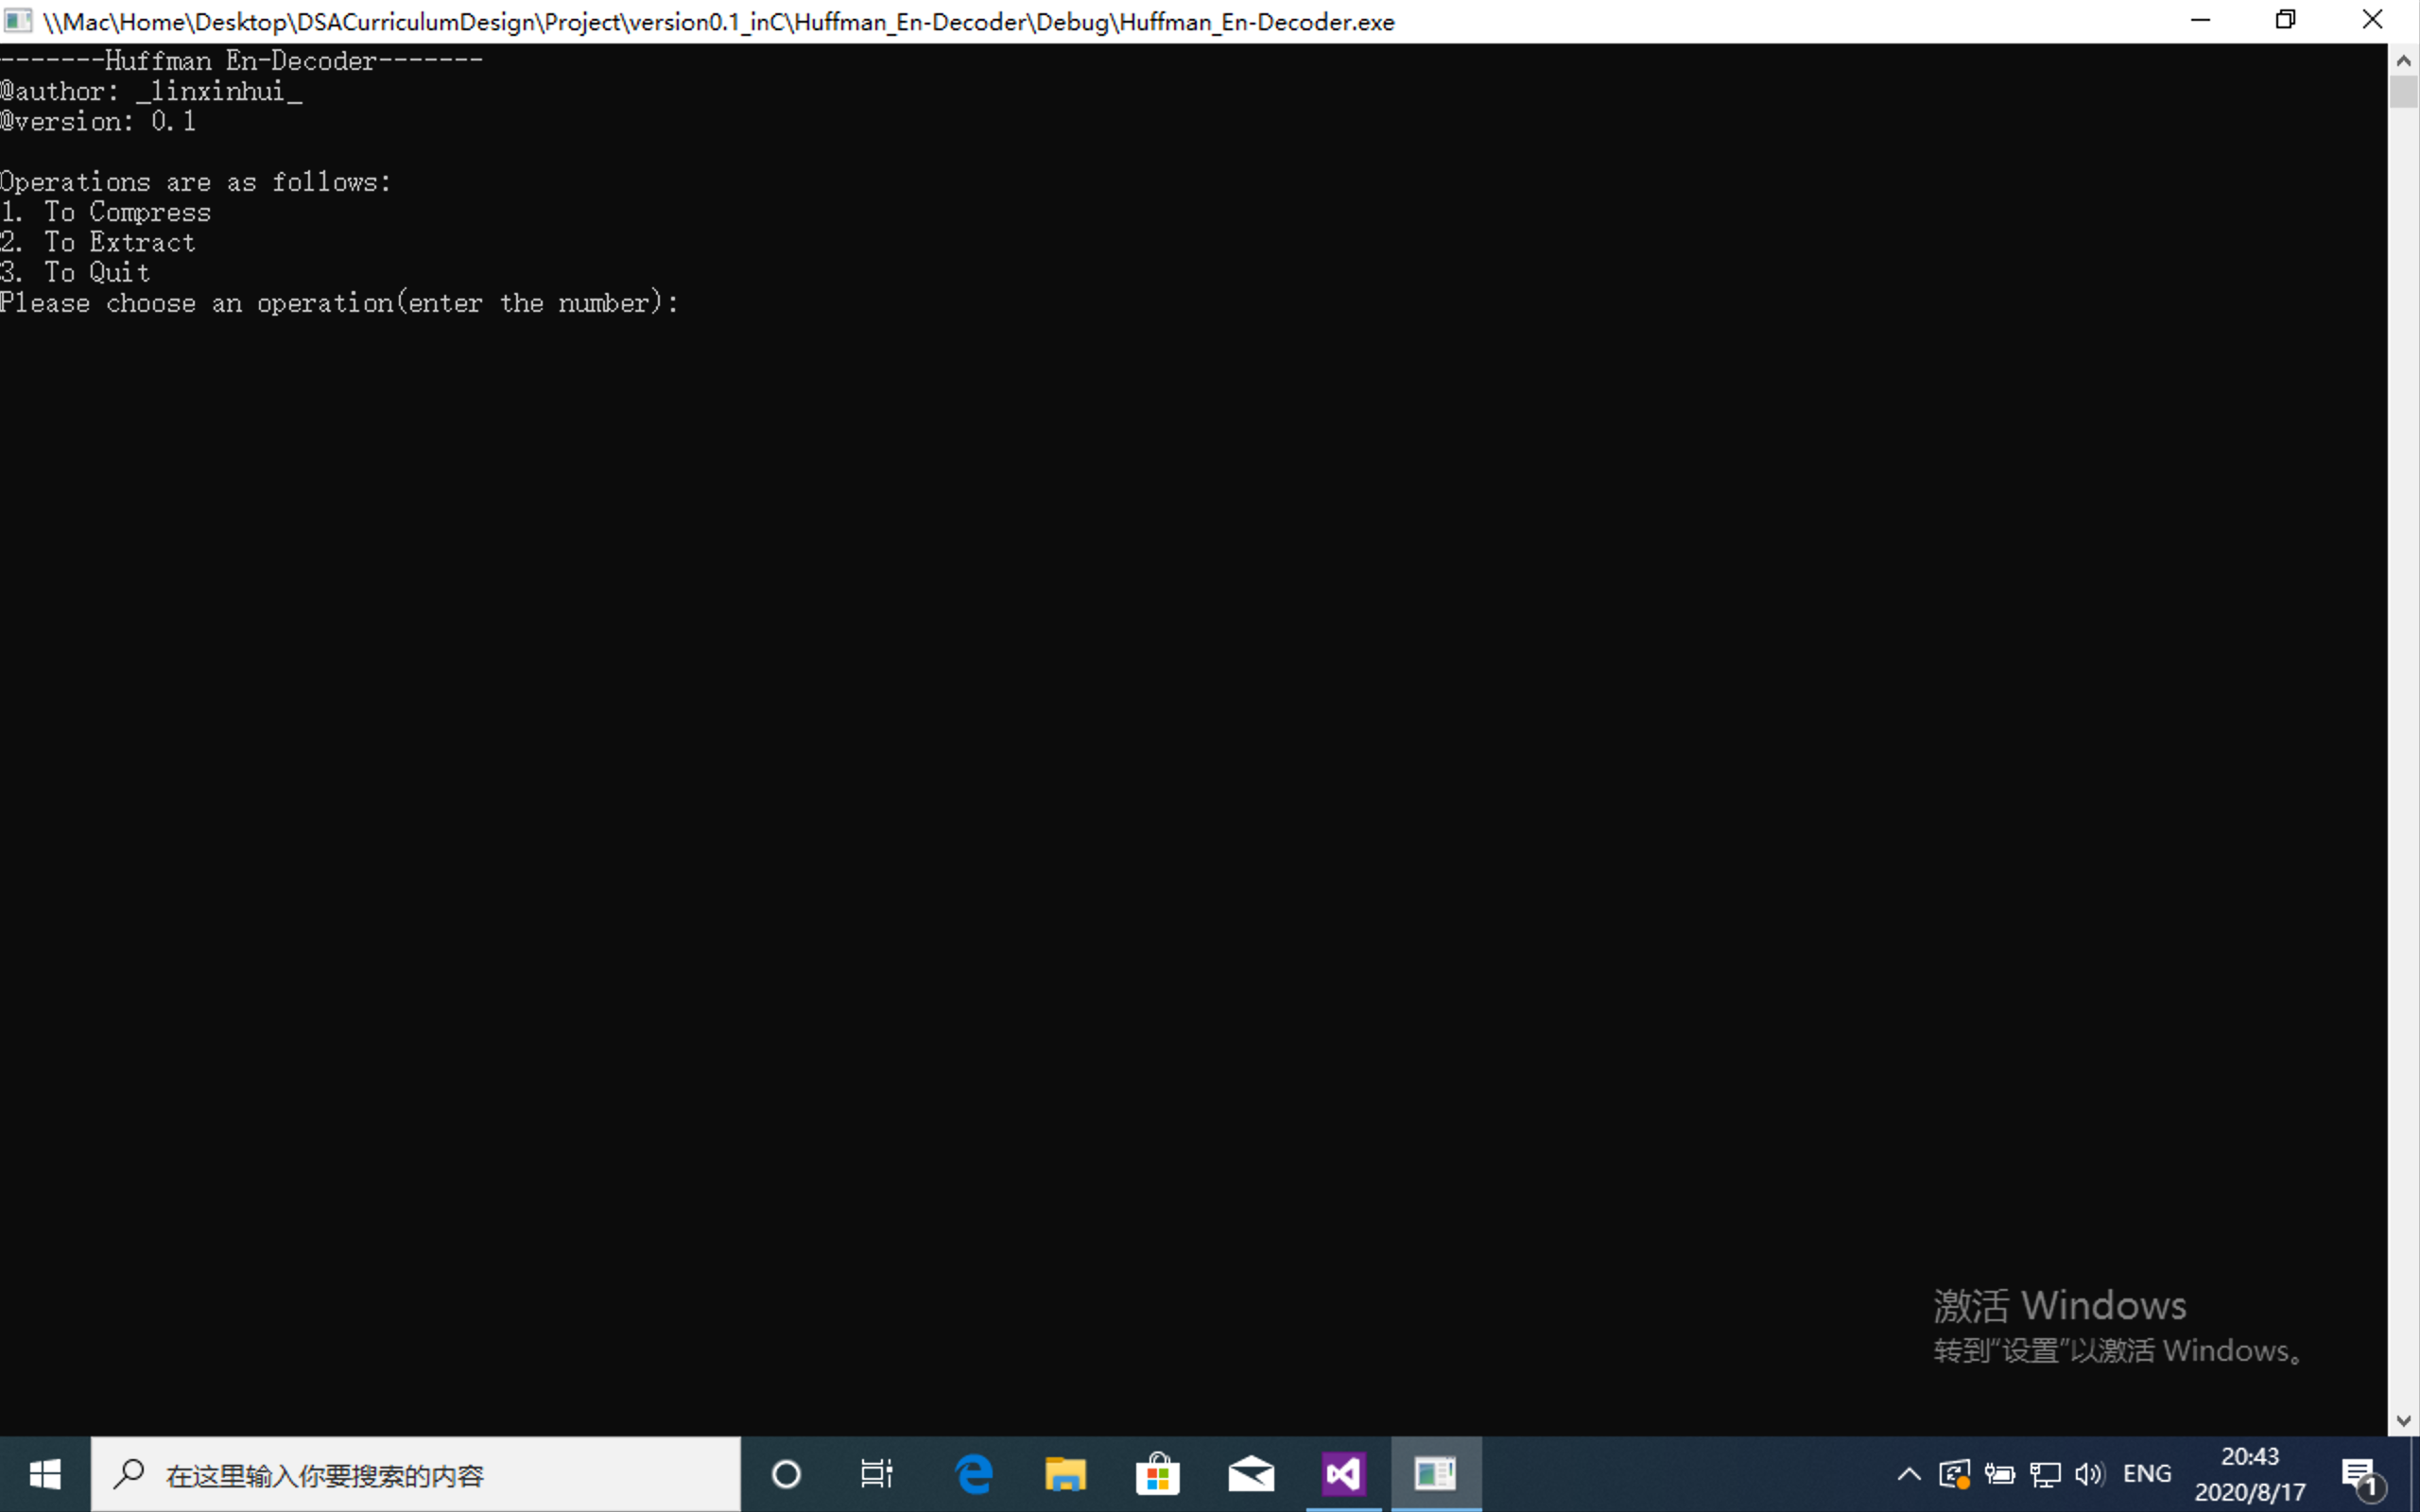
\includegraphics[scale=0.1]{../ComputationalResultsScreenshot/C/01_交互信息(主界面).png}
\caption{C版本交互信息通过终端呈现}
\end{figure}

\begin{figure}[H]
\centering
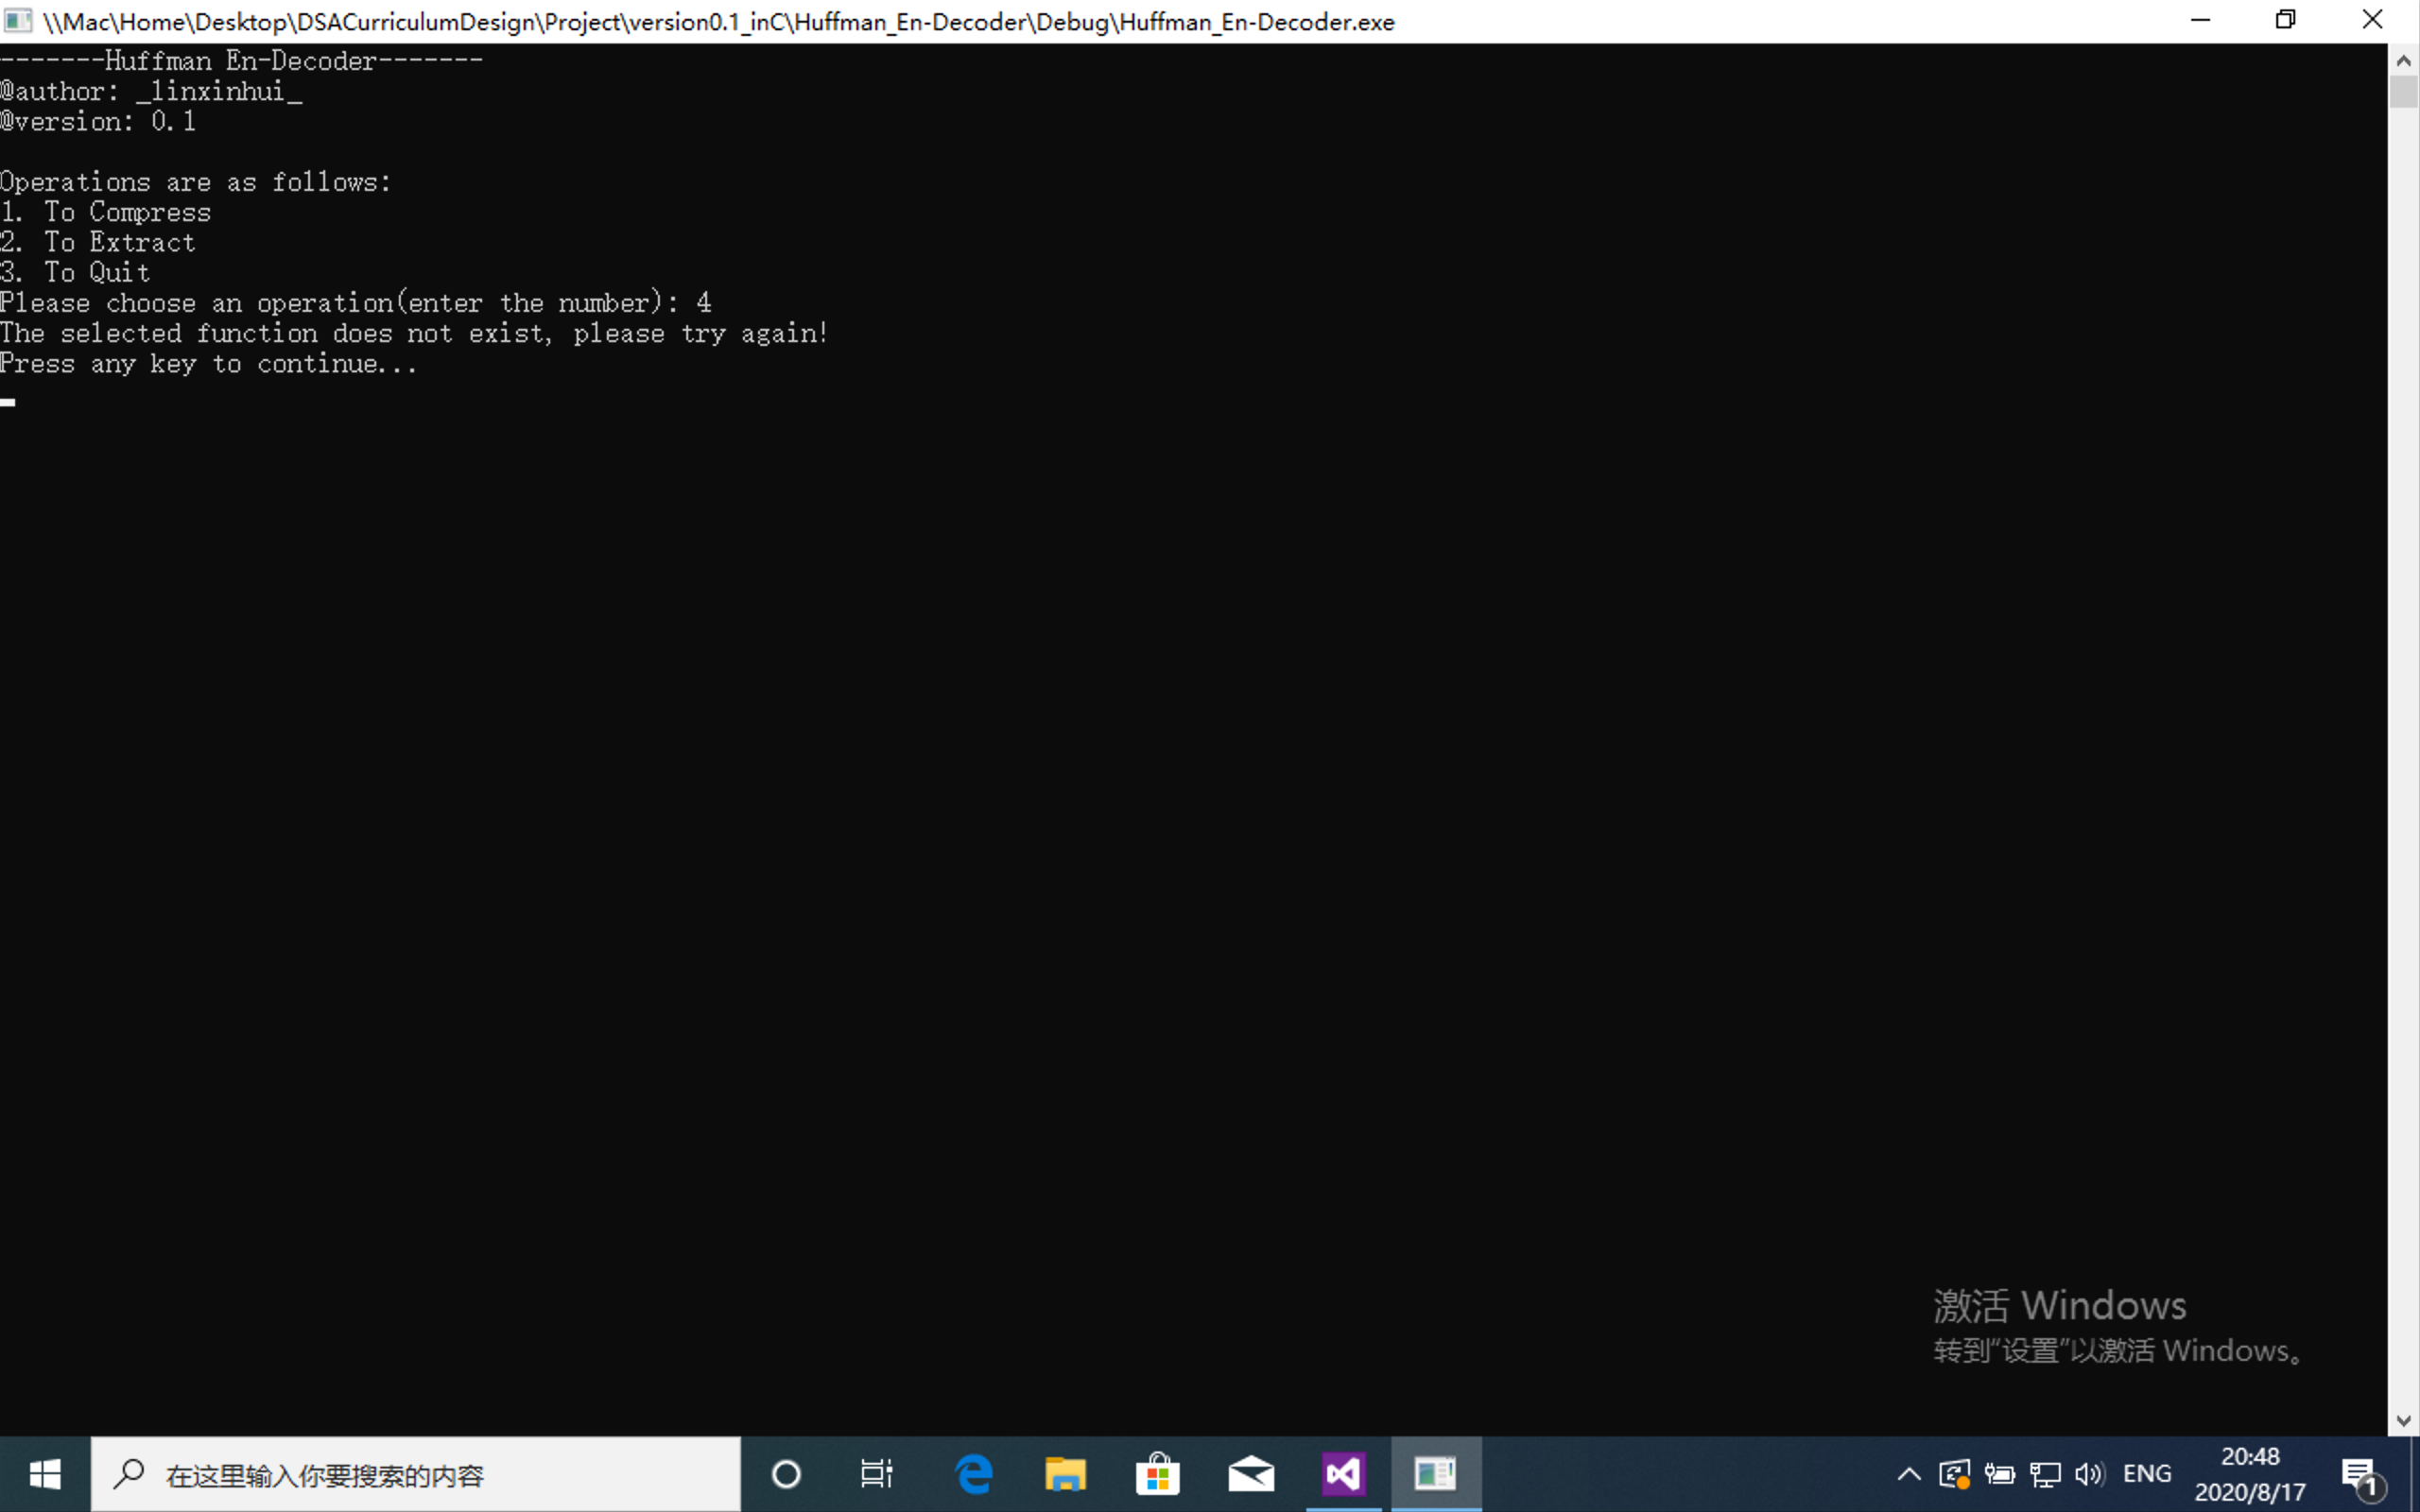
\includegraphics[scale=0.1]{../ComputationalResultsScreenshot/C/03_输入错误.png}
\caption{提示输入错误}
\end{figure}

\begin{figure}[H]
\centering
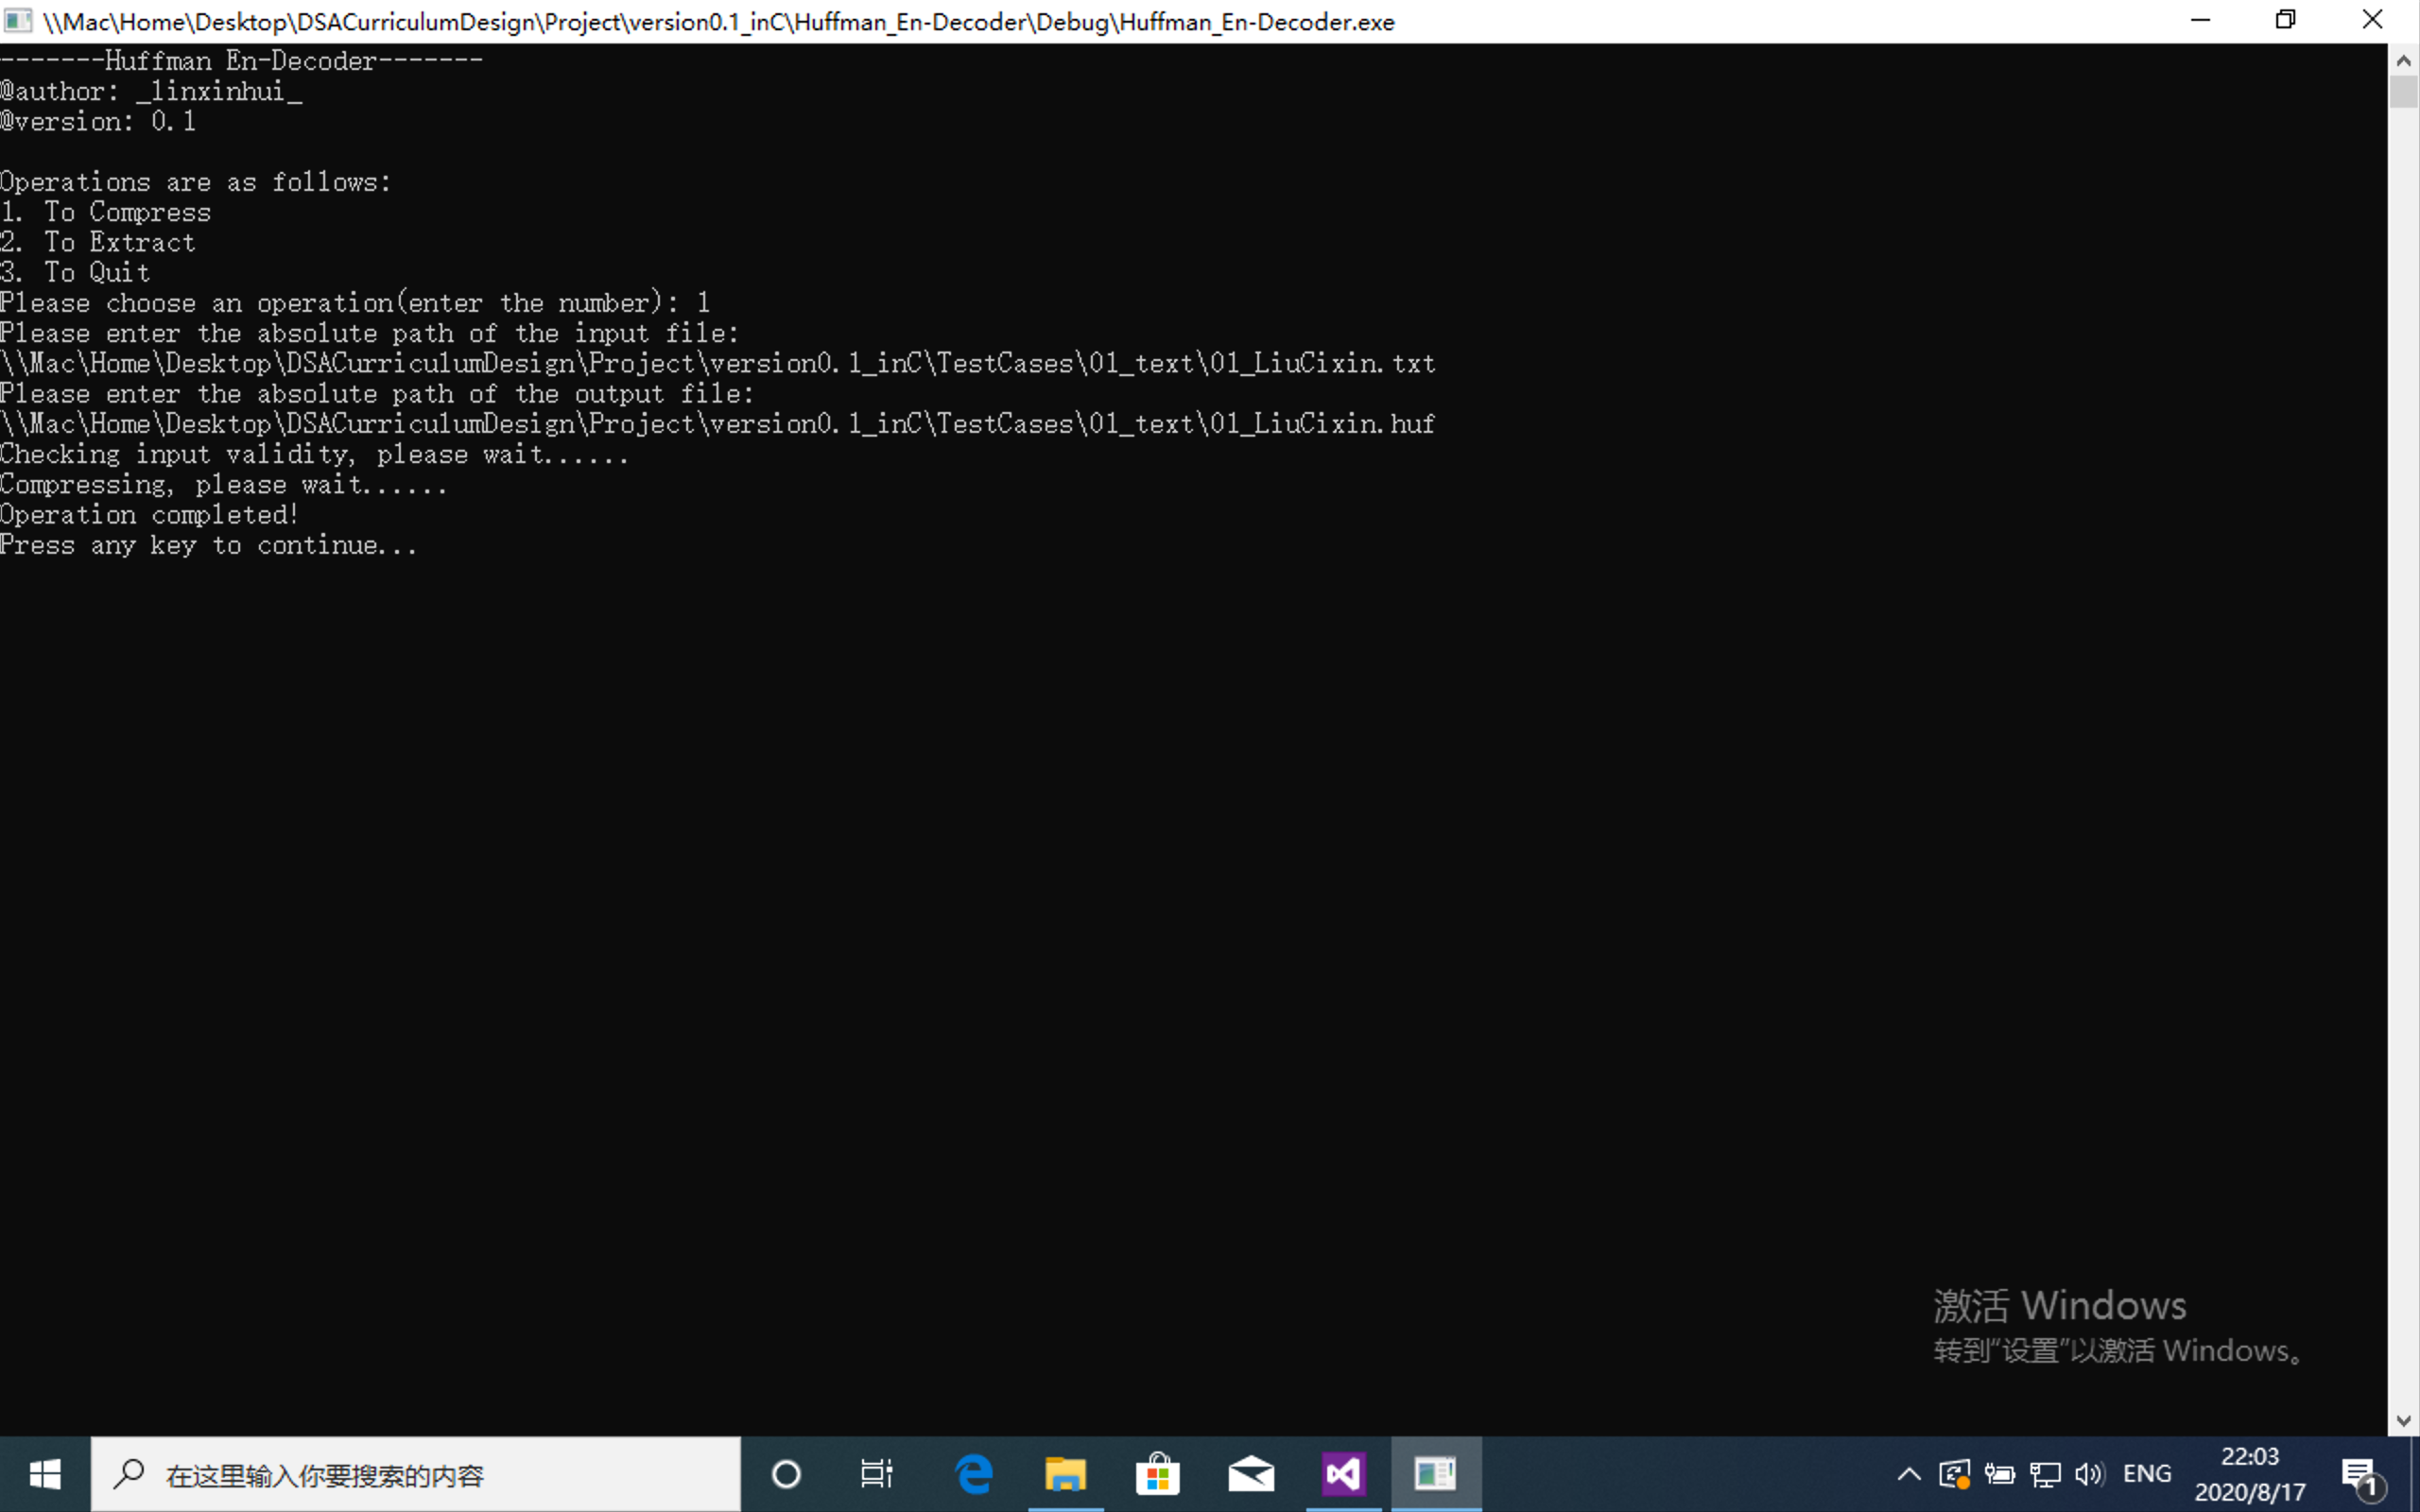
\includegraphics[scale=0.1]{../ComputationalResultsScreenshot/C/04_压缩过程.png}
\caption{加载编码/压缩模块}
\end{figure}

\begin{figure}[H]
\centering
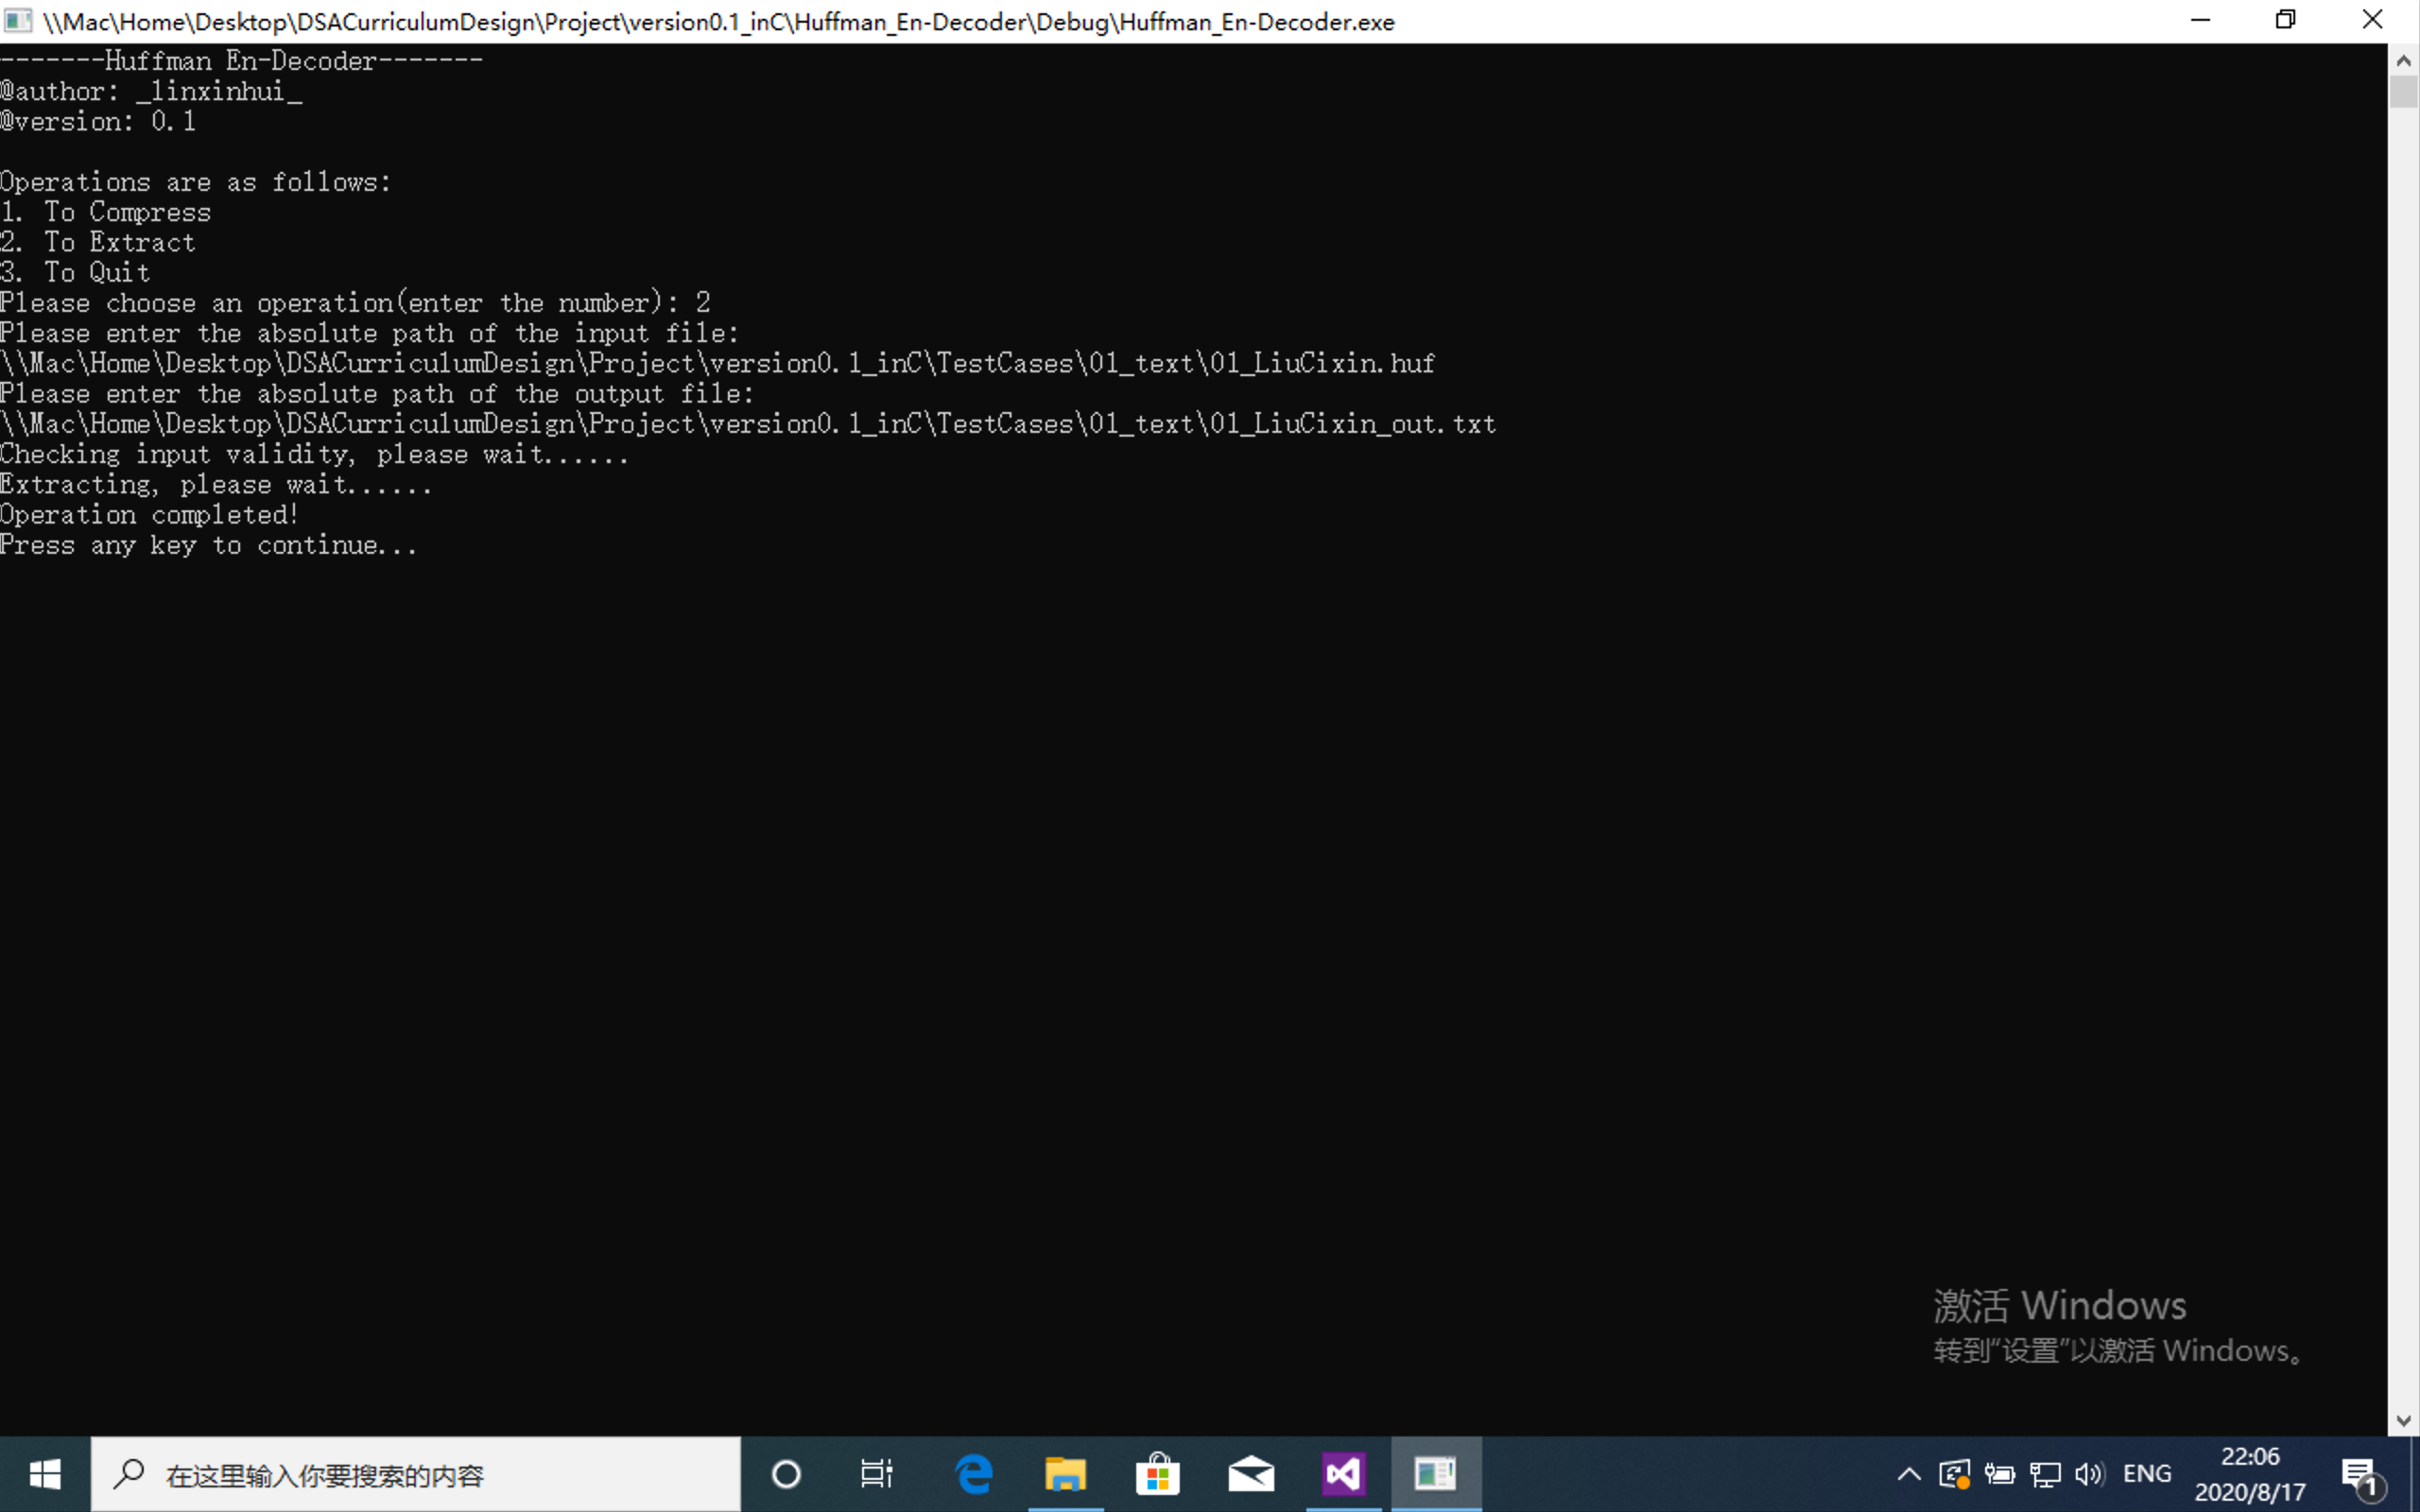
\includegraphics[scale=0.1]{../ComputationalResultsScreenshot/C/05_ 解压缩过程.png}
\caption{加载解码/解压缩模块}
\end{figure}

\begin{figure}[H]
\centering
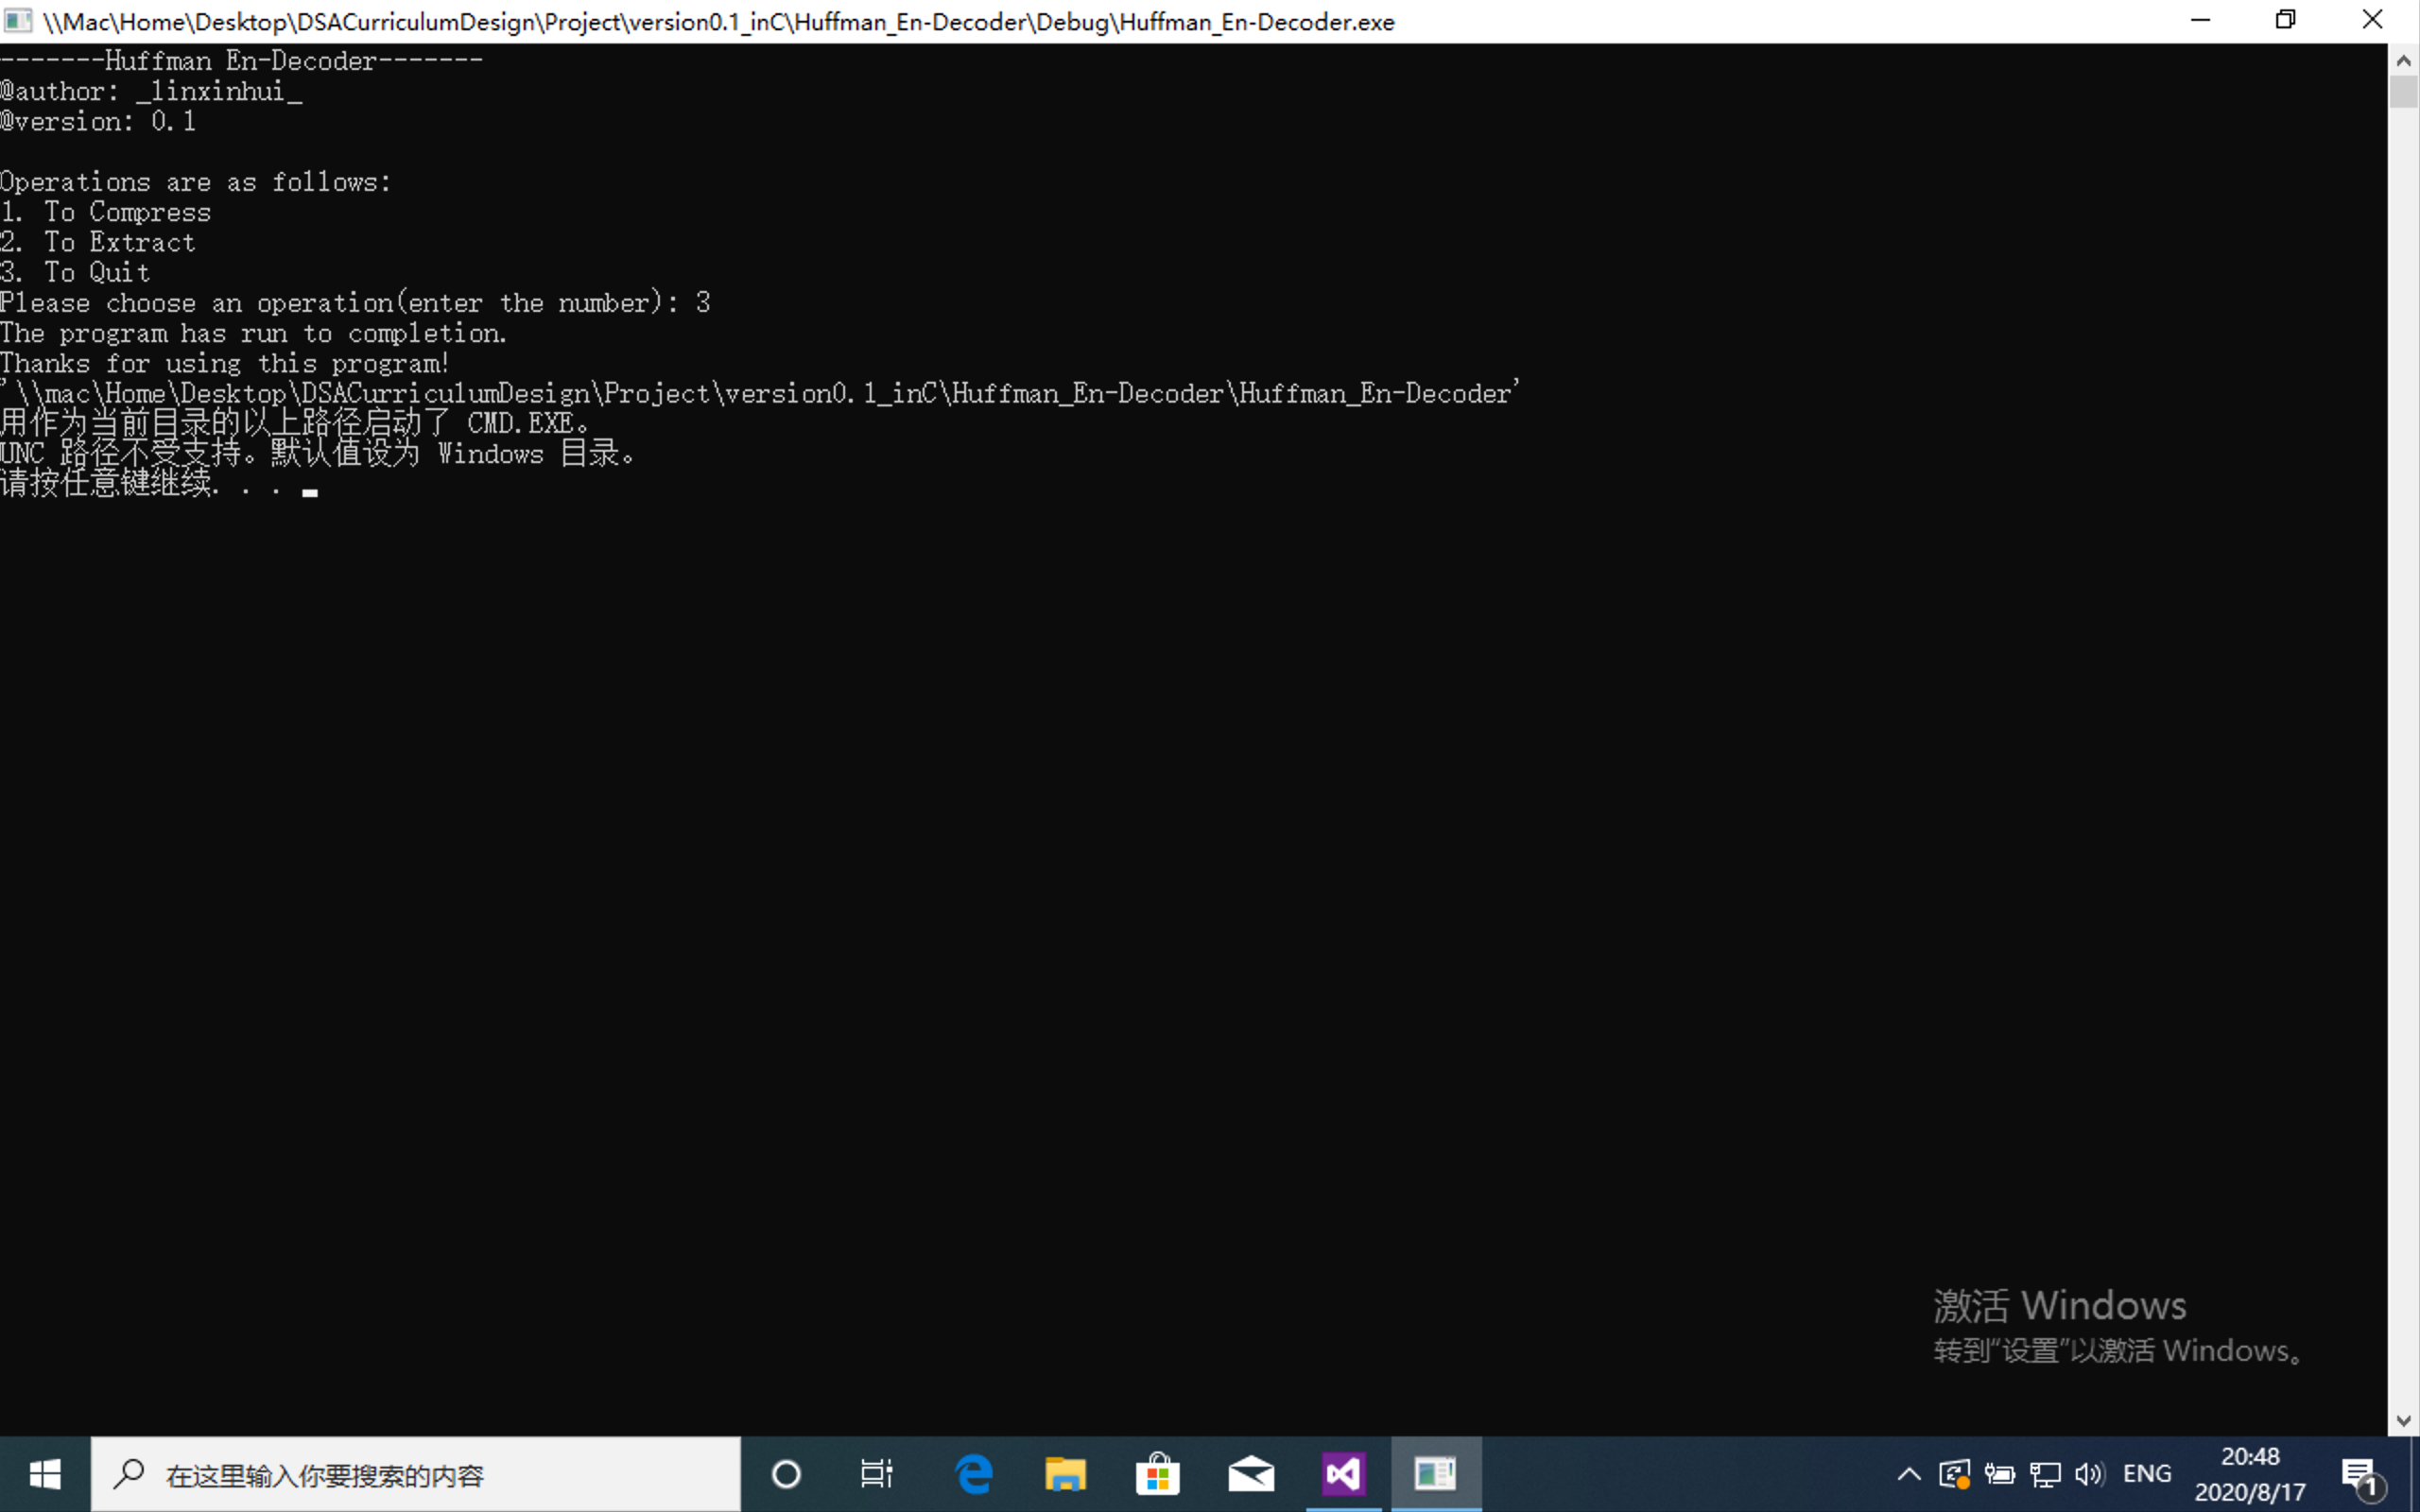
\includegraphics[scale=0.1]{../ComputationalResultsScreenshot/C/02_退出.png}
\caption{退出程序}
\end{figure}

\begin{figure}[H]
\centering
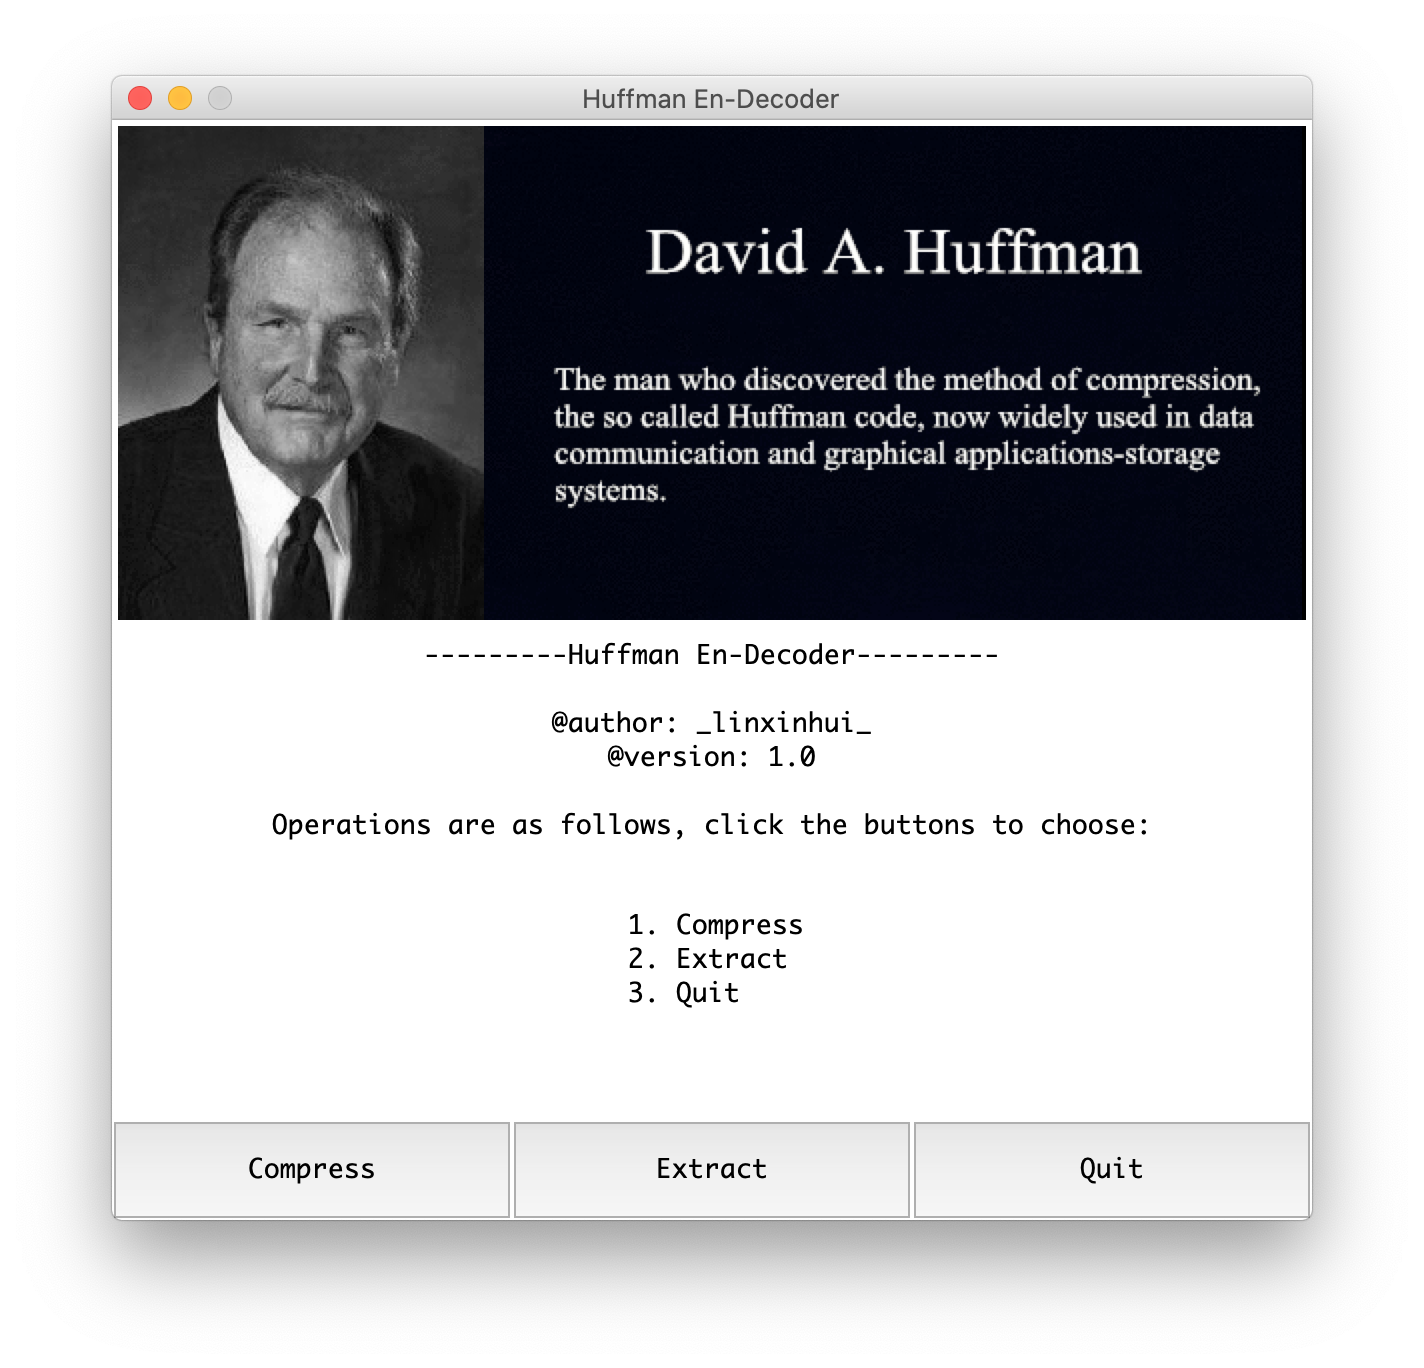
\includegraphics[scale=0.4]{../ComputationalResultsScreenshot/Python/01_主窗口.png}
\caption{Python版本有了用户图形界面}
\end{figure}

\begin{figure}[H]
\centering
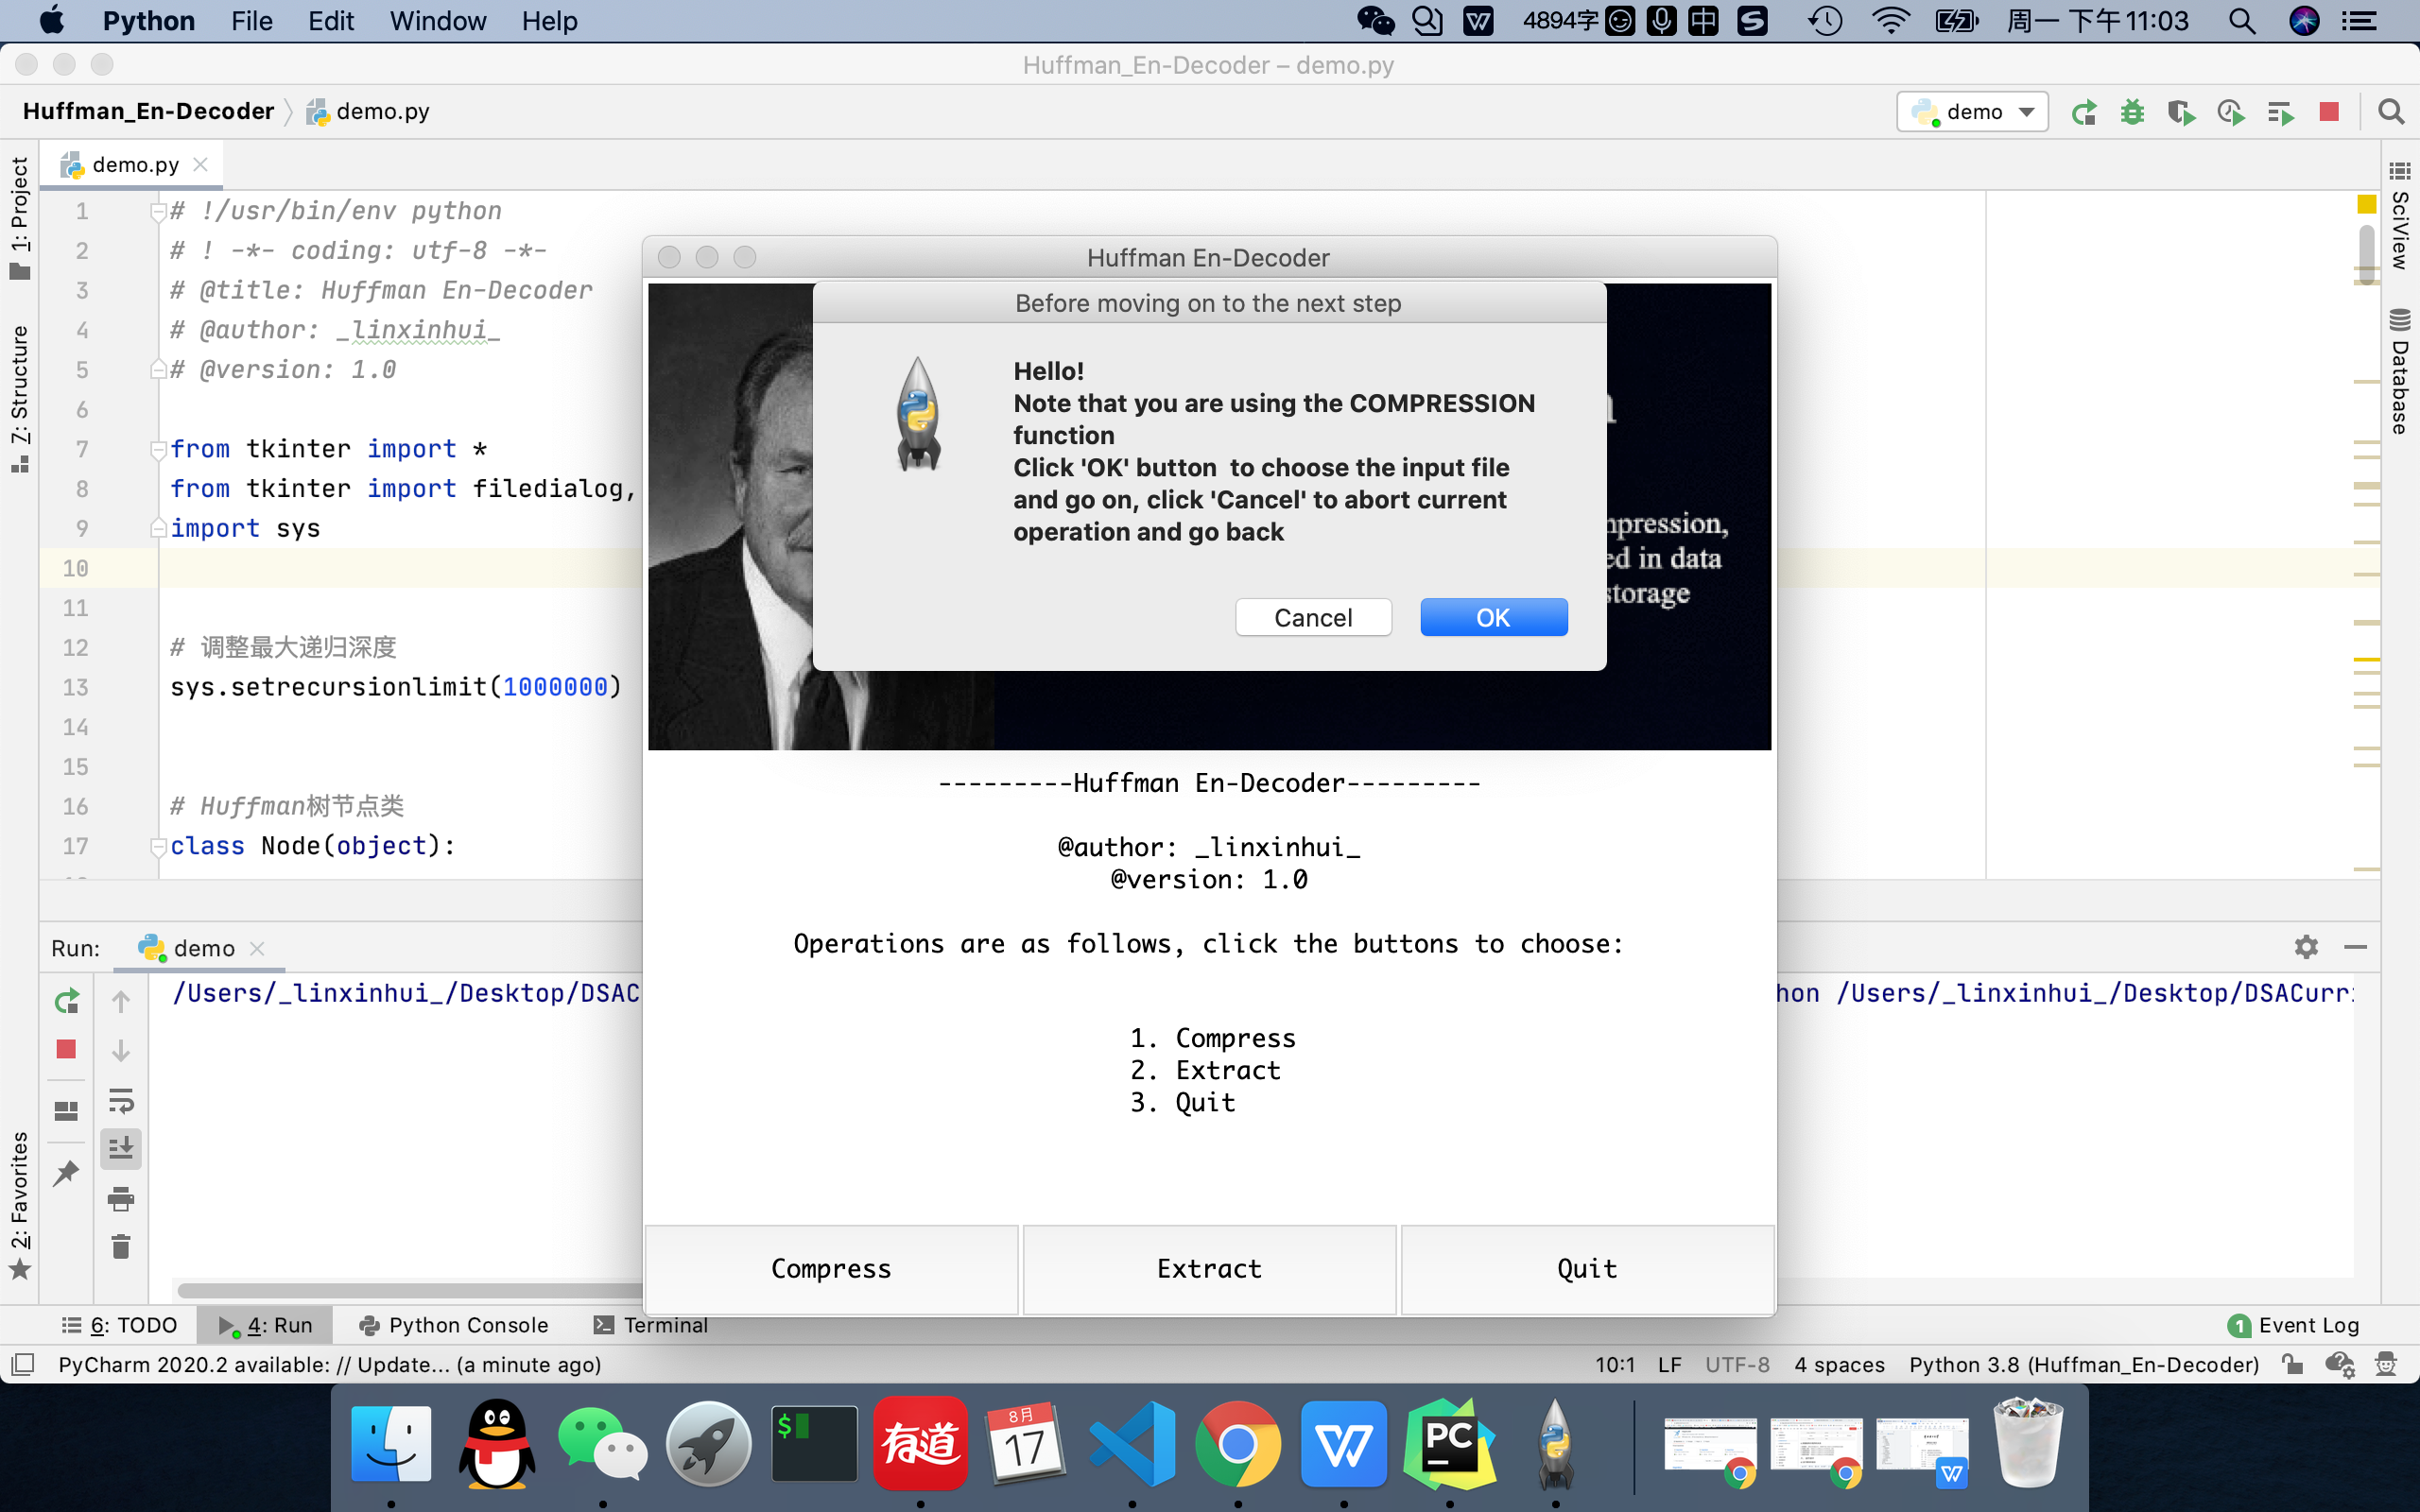
\includegraphics[scale=0.2]{../ComputationalResultsScreenshot/Python/02_消息窗口_确认开始压缩.png}
\caption{确认开始压缩}
\end{figure}

\begin{figure}[H]
\centering
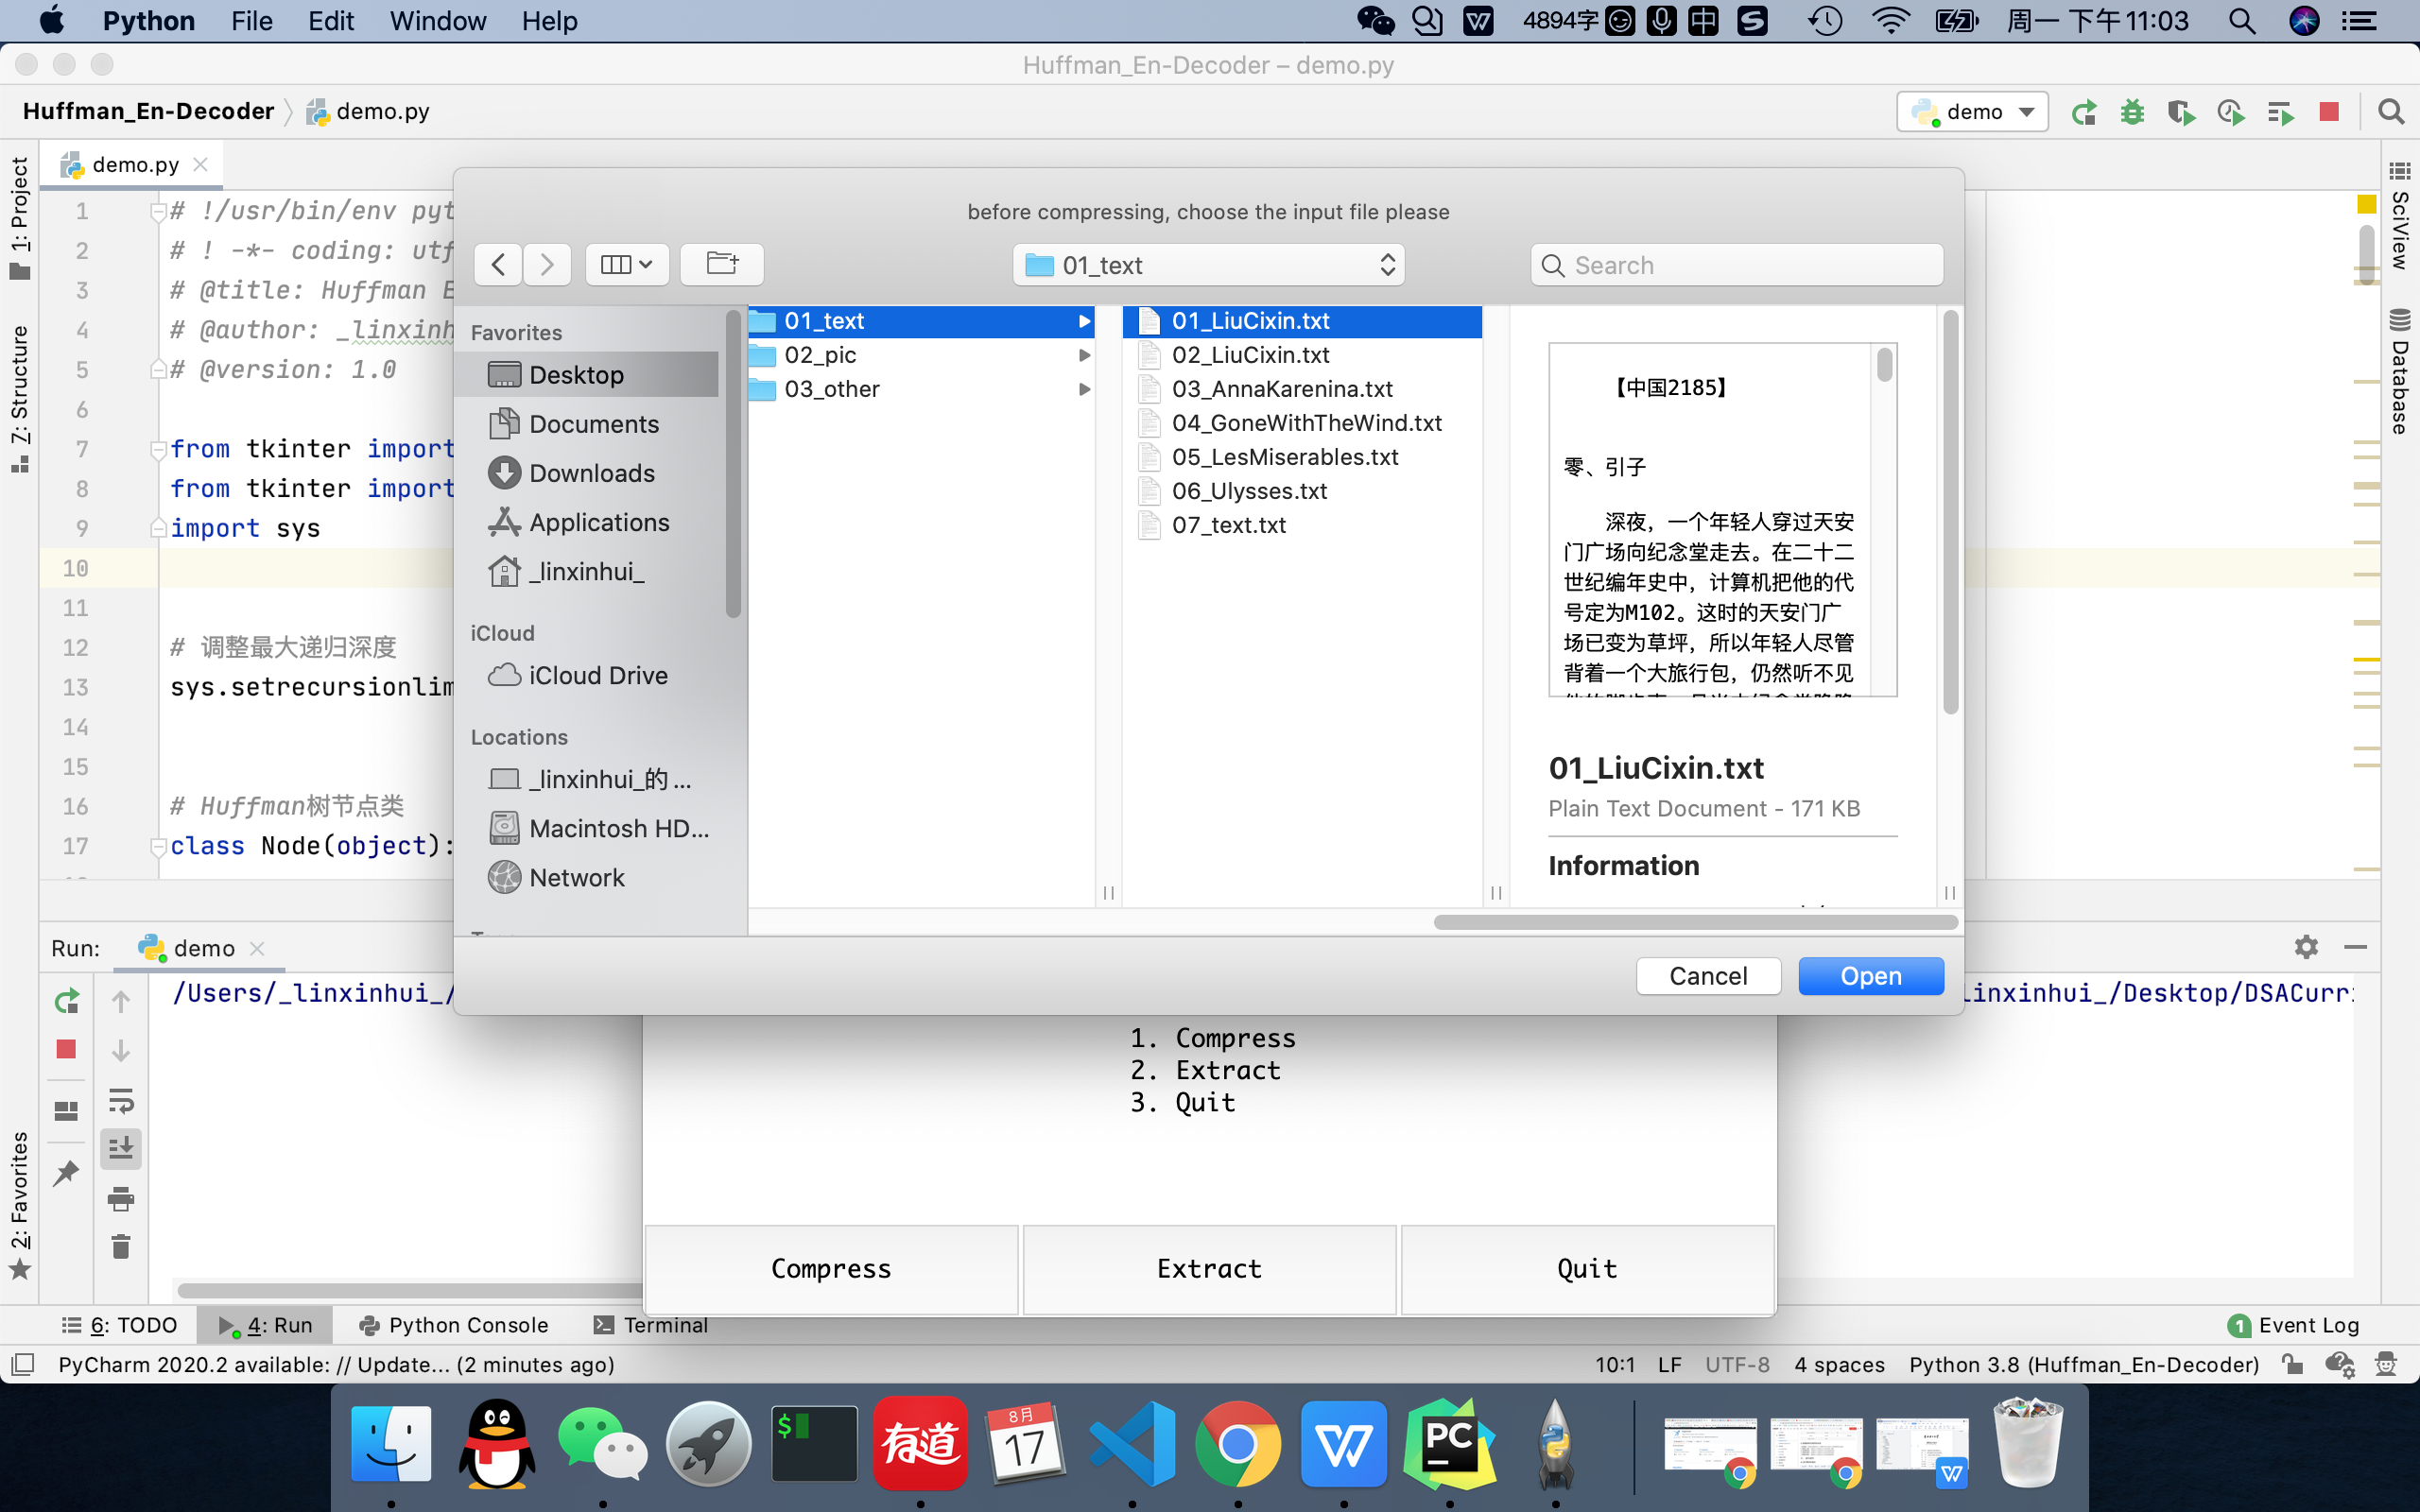
\includegraphics[scale=0.2]{../ComputationalResultsScreenshot/Python/03_消息窗口_选择文件.png}
\caption{选择待压缩文件}
\end{figure}

\begin{figure}[H]
\centering
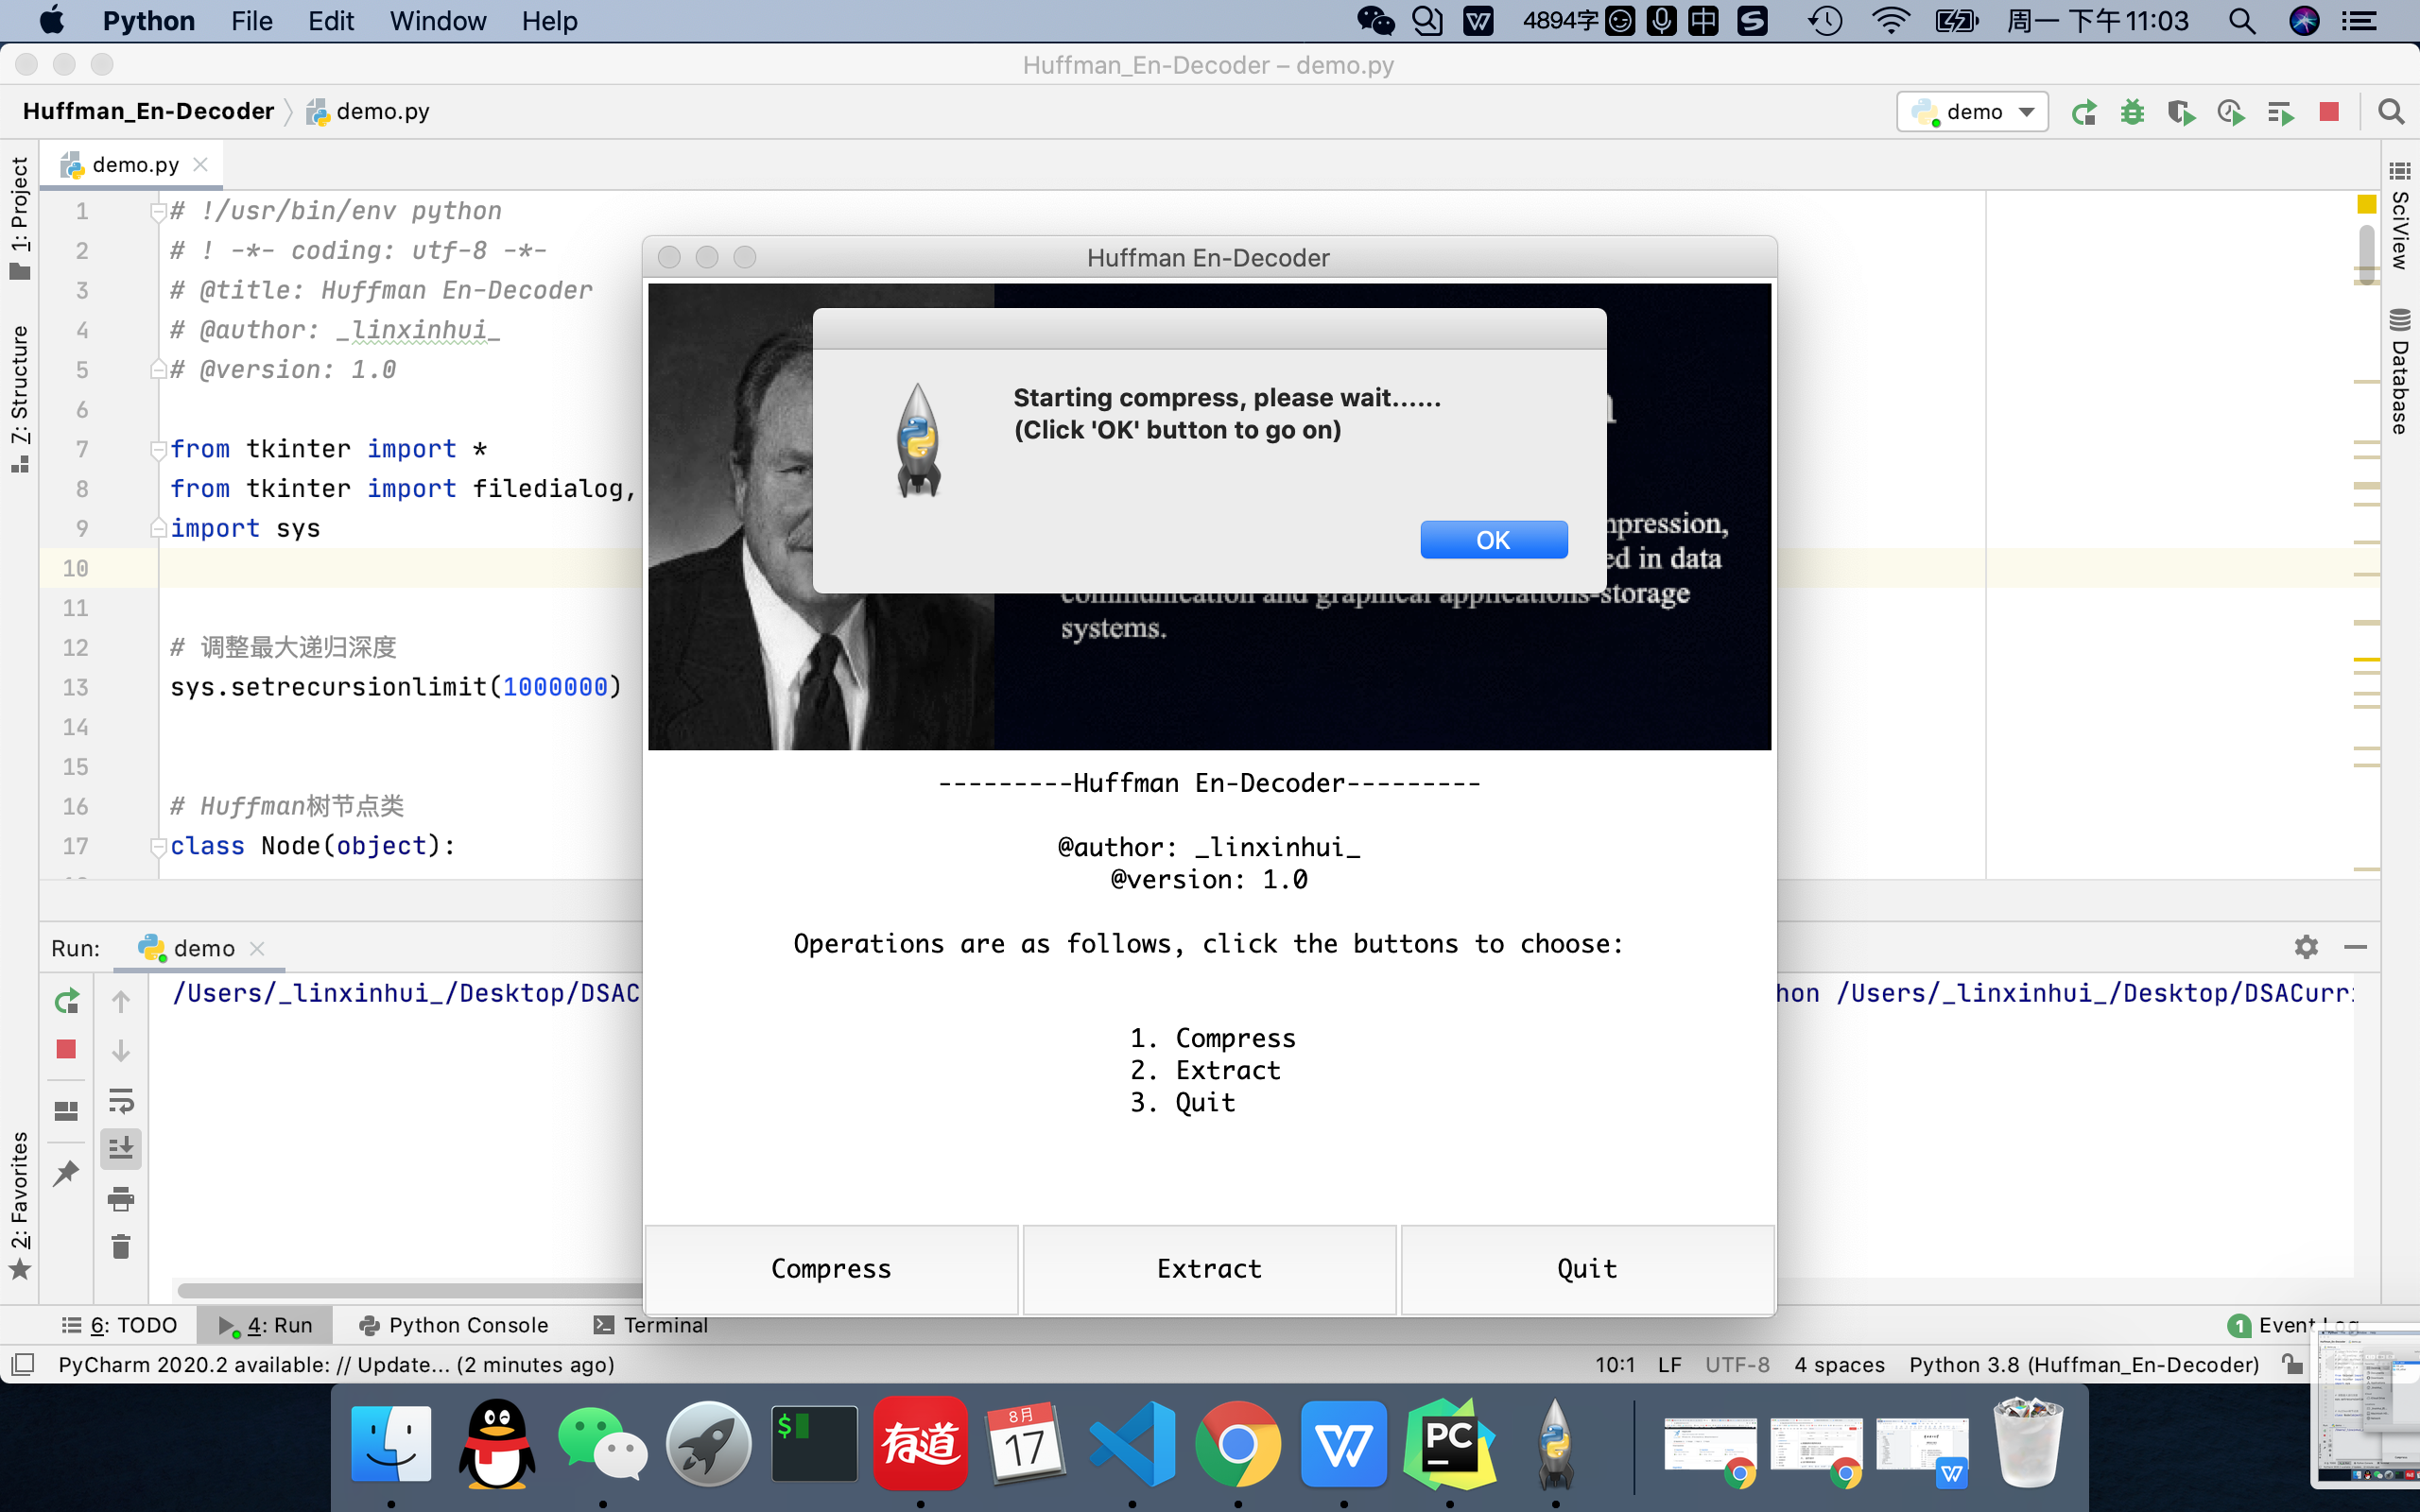
\includegraphics[scale=0.2]{../ComputationalResultsScreenshot/Python/04_消息窗口_提示正在压缩.png}
\caption{正在压缩}
\end{figure}

\begin{figure}[H]
\centering
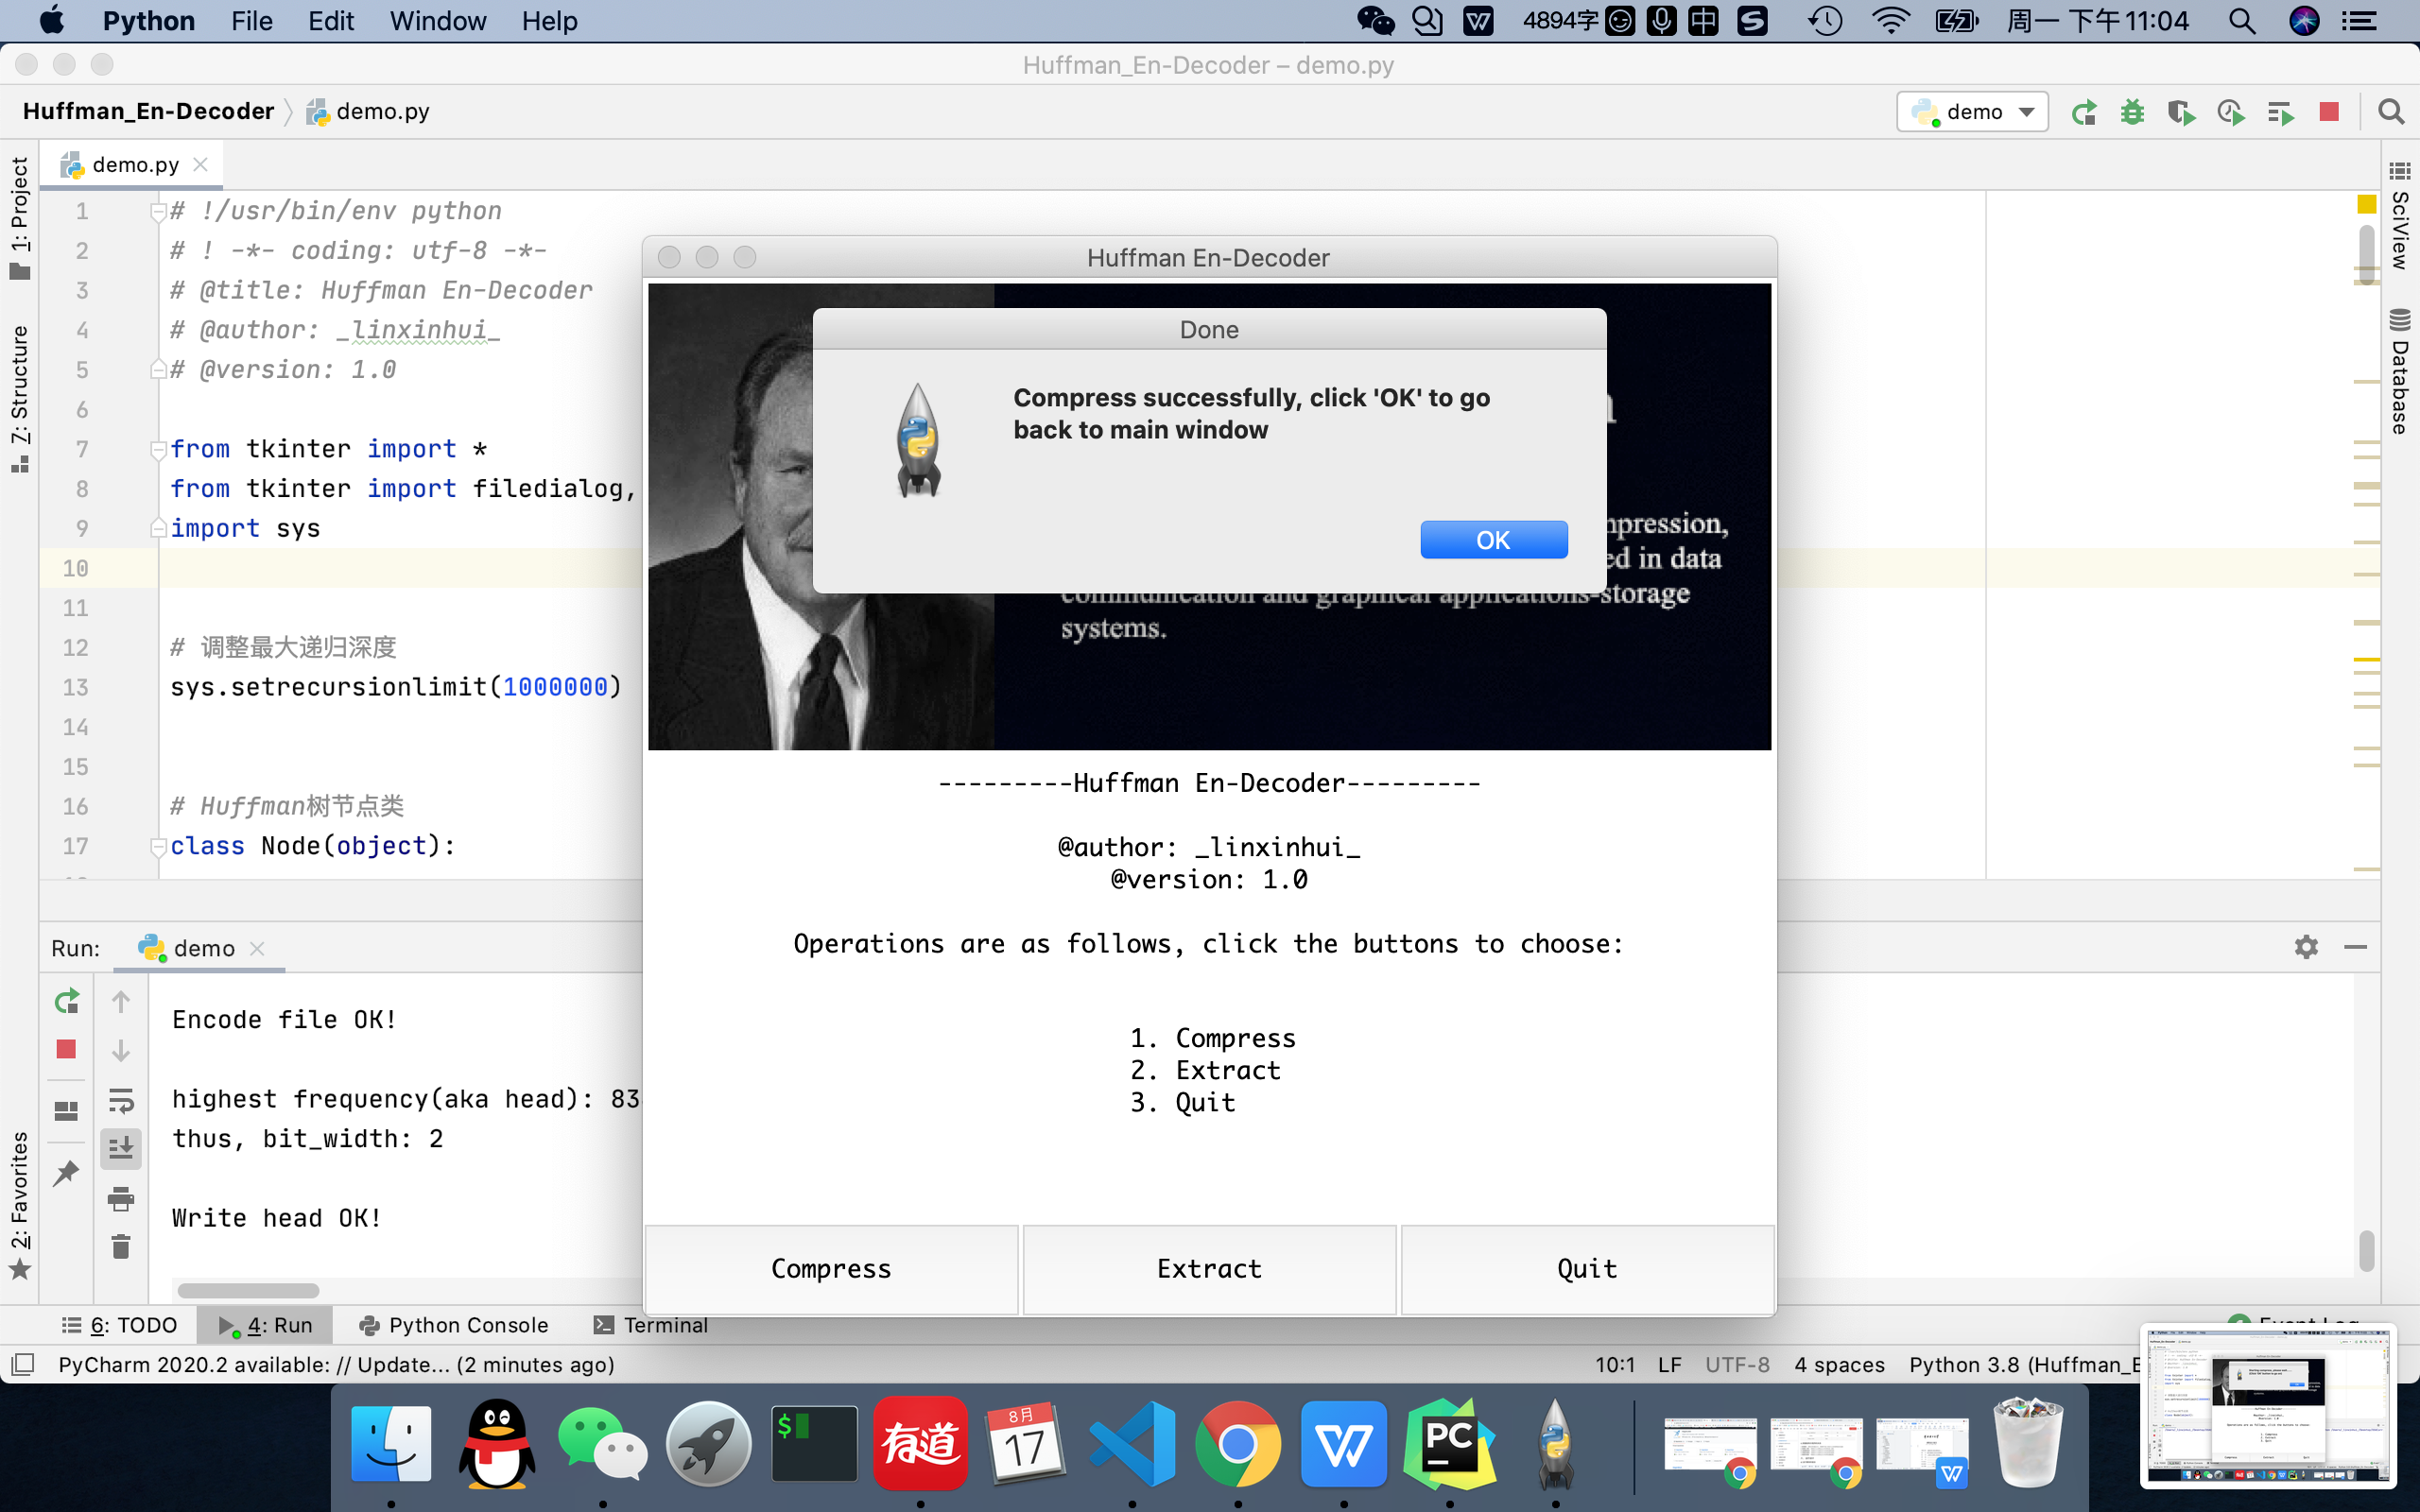
\includegraphics[scale=0.2]{../ComputationalResultsScreenshot/Python/05_消息窗口_提示压缩完成.png}
\caption{压缩完成}
\end{figure}

\begin{figure}[H]
\centering
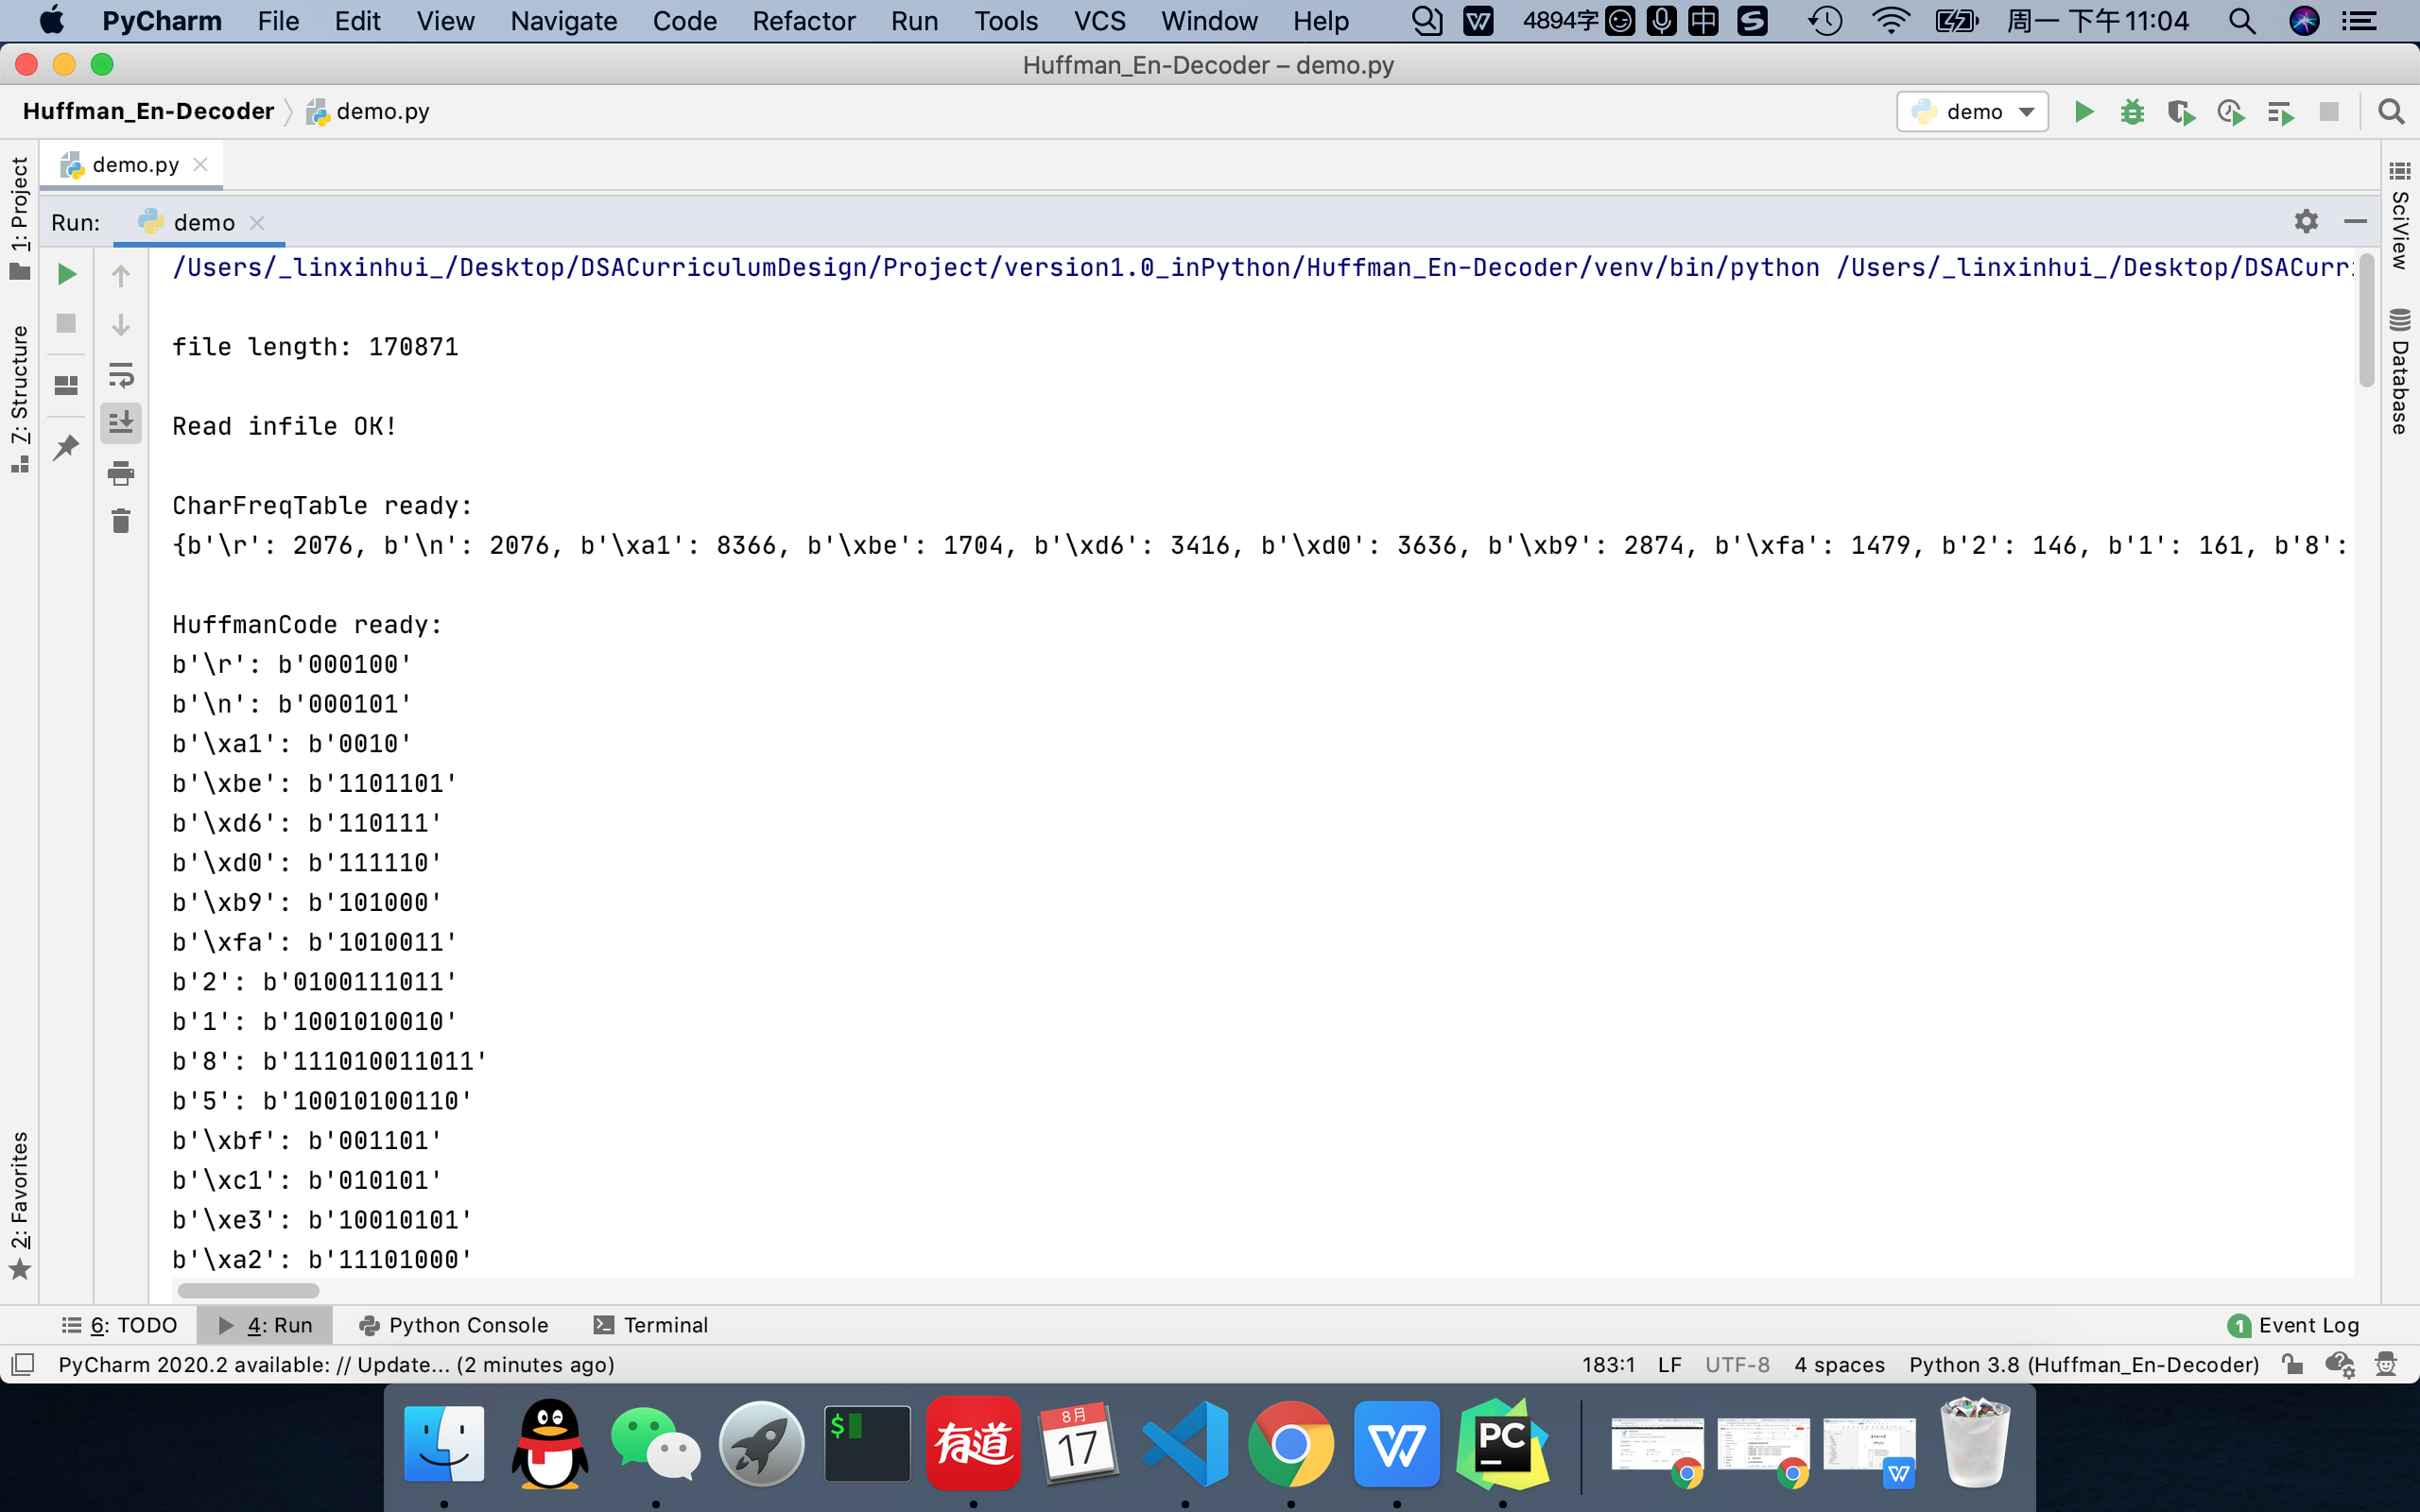
\includegraphics[scale=0.2]{../ComputationalResultsScreenshot/Python/06_输出调试信息01.png}
\caption{输出调试信息}
\end{figure}

\begin{figure}[H]
\centering
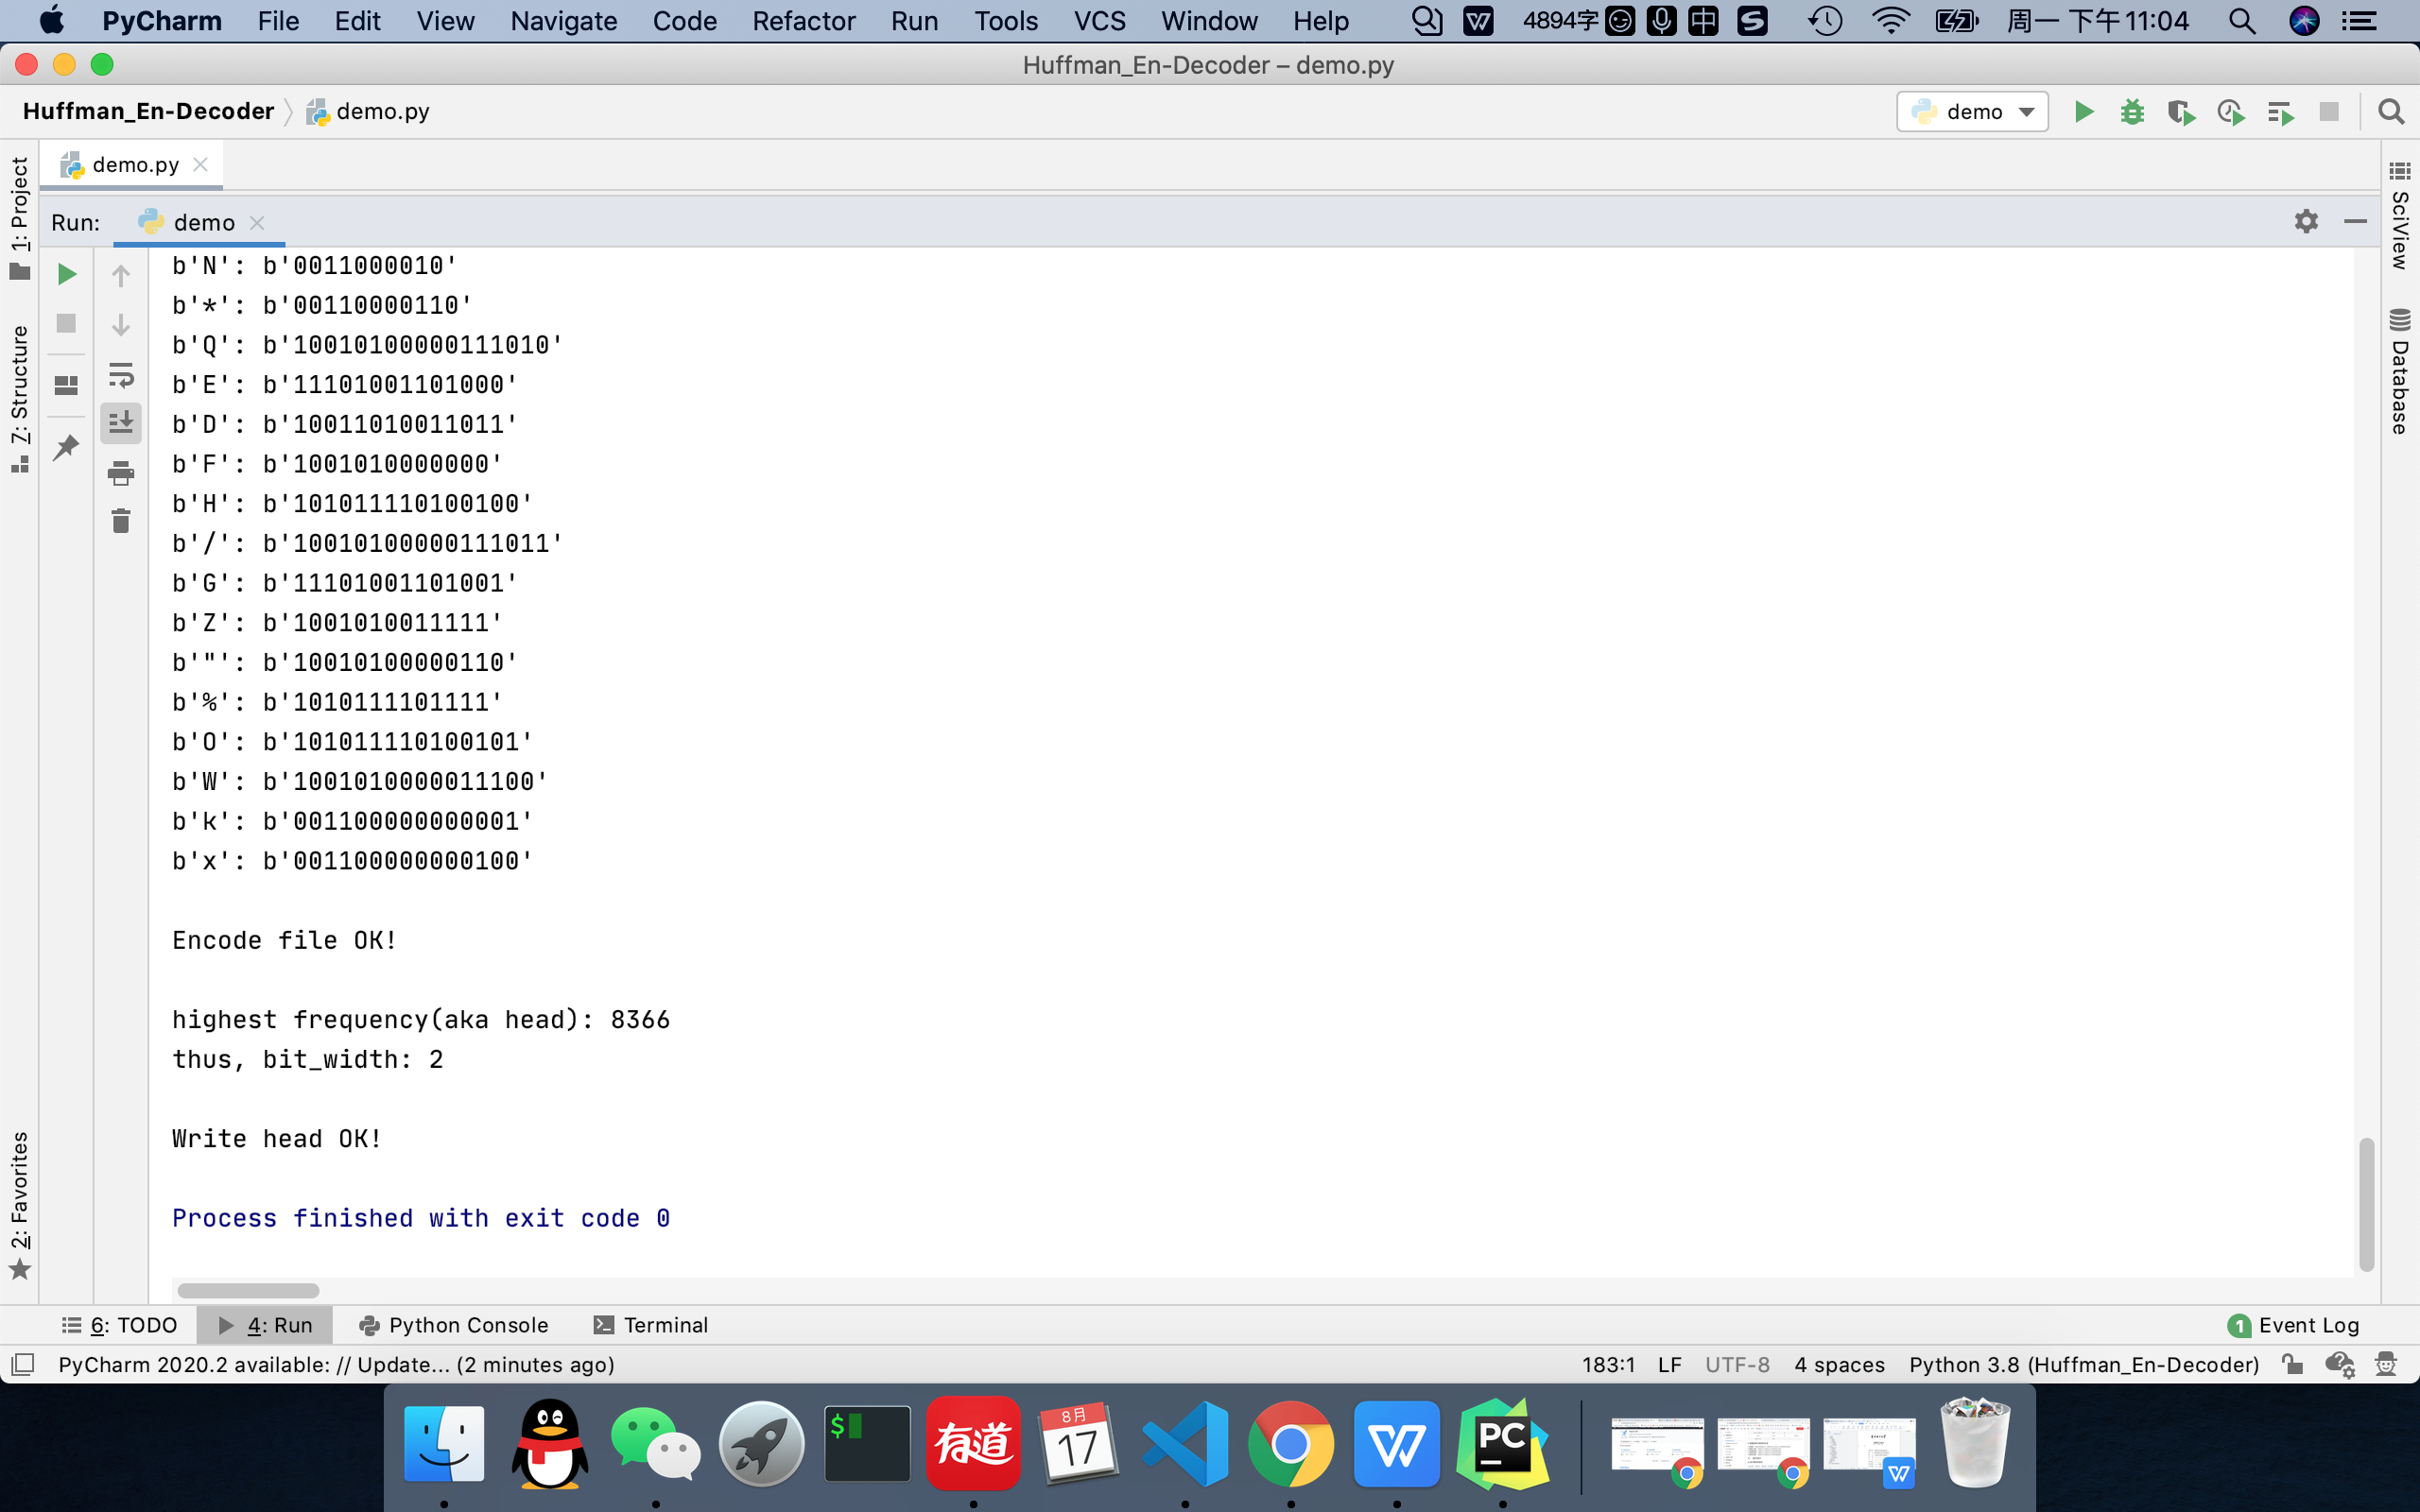
\includegraphics[scale=0.2]{../ComputationalResultsScreenshot/Python/07_输出调试信息02.png}
\caption{输出调试信息}
\end{figure}

解压缩过程的步骤与压缩过程完全一致, 不重复贴图了。

大版本\texttt{version0.2}和\texttt{version1.0}中包含\texttt{TestCases}文件夹提供测试样例, 对文本、图片、音频进行压缩, 每个文件一式三份, 包括原文件(xx.yy)、压缩文件(xx.huf)、解压文件(xx\_out.yy)。

文本文件包括\texttt{.txt}文件, \texttt{.c}文件, \texttt{.h}文件, \texttt{.py}文件和\texttt{.md}文件(文本文件的内容中英文符号都有)。

图片包括\texttt{.gif}文件, \texttt{.jpg/.jpeg}文件, \texttt{.png}文件和\texttt{.bmp}文件。

音频只测试了\texttt{.mp3}文件。

还有其他格式文件包括\texttt{.pdf}文件, \texttt{.doc}文件, \texttt{.exe}文件。

以上列举的都是主流文件格式, 两个版本都能正确地编码、解码。其他文件格式理论上都是可以压缩的, 有兴趣可以自行尝试。

简单分析一下压缩率, 首先要说明的是编解码器对所有格式都能实现编解码, 不意味着对所有文件都能实现压缩。分析测试样例中给出的数据可以发现有如下规律:

\begin{enumerate}
\def\labelenumi{\arabic{enumi}.}
\item
  编解码器对文本文件基本能实现压缩。事实上, 若文件中的字符数量很少, 并且重复次数不多, 由于写入的文件头也需要占用一定的内存, 可能导致压缩率及其不理想, 甚至有压缩文件比原文件更大的情况
\item
  还是文本文件, 文本文件越大, 压缩率越理想, 且英文文本的压缩率比中文文本理想, 一般的英文文本的压缩率通常可以达到50\%, 中文往往只有75\%
\item
  对于特殊的文本文件, 具体地说, 就是文本中只包含一种字符, 且字符重复了很多遍的情况下, 压缩率几乎可以趋近于0, 不过这种场景几乎不存在
\item
  对于图像(对\texttt{bmp}文件还能实现压缩)、音频, 以及pdf文档和word文档等文件格式, 使用Huffman算法压缩的压缩率可以说惨不忍睹了,编码后的文件与原文件的大小几乎相同(甚至更大), 此时应用Huffman算法的过程只能被称为编码, 不能被称为压缩
\end{enumerate}

综上, 对包含字符少且字符重复次数多的文件使用Huffman编码, 往往能取得较好的结果。通过查阅资料知道,
\texttt{MPEG}、\texttt{JPEG}格式的文件在生成的过程中使用了自适应Huffman码, \texttt{gif}文件是由LZW算法压缩得到的, \texttt{pdf}文件、\texttt{word}文件同理, Huffman算法对于这类本身已经经过压缩的文件格式基本无效。

最后说一句, 由于不知道什么原因的原因, \texttt{Python版本}的解码器使用完一次后必须重启才能正常解码(编码器没有这种问题), 在使用时请注意。

%—— 6 课程设计总结

\section{课程设计总结}\label{header-n431}

首先对本次课程设计做个总结。

本课程设计从规划到完成耗时一个半月, 期间遇到的各种各样的从算法设计到语言细节到交互设计到文档书写的各种各样的问题不必多说。这个项目不算大, 无论是比于商业级别的压缩软件还是正儿八经的Huffman编解码器的实现都显得简陋而蹩脚, 它的压缩/解压缩速度和压缩率很难令人满意, 它作为Huffman编解码器的实现也谈不上体现Huffman算法的优越性, 但这确实几乎是我做过的最大型的项目, 实现过最完整的功能, 实现它,
我自认为达到了课程设计目的与要求:

\begin{enumerate}
\def\labelenumi{\arabic{enumi}.}
\item
  了解熟练掌握编程开发工具, 加强调试功能, 掌握跟踪、修改错误的技巧。
\item
  能根据实际问题进行数据结构的选用、算法设计与分析、程序设计与实现
\item
  进一步加强和提高文档报告的编写能力
\item
  在不断调试程序过程中培养坚强的毅力以及不怕困难、精益求精的大国工匠精神
\end{enumerate}

压缩技术发展到今天, 各种先进的算法层出不穷, 但Huffman算法依然是最好的压缩算法之一。

Huffman编码是熵编码的一类, 这决定了其编解码的速度实际是很快的(在本课设中这一点体现得并不显著,
主要是受到读写方式的影响), 远远强于算数编码和字典编码。

Huffman编码单独使用的场景不多, 一般作为压缩算法的一环出现, 这样的例子有很多, 比如作为互联网基础标准之一的rfc1951中的最后一层压缩就是使用Huffman编码的, png/gz/zip/JPEG/http中都以1951为引用,
所以这些文件的背景都有Huffman编码的影子, 又如DEFLATE是同时使用了LZ77算法与Huffman编码的一种无损数据压缩算法(具体地说是使用字典编码将输入的数据量降下来, 再使用huffman、arc之类的熵编码器输出最终压缩好的数据)等等, 其应用的广泛性可见一斑。本段内容来源于互联网, 整合自几个有着数据压缩领域背景的前辈关于Huffman应用的讨论, 这些算是Huffman编码的应用限于能力目前肯定是无法实现的(事实上理解原理都很困难), 未来有机会也许作为一个方向研究研究, 而本次课程设计就作为一个引子, 作为进一步研究的基础。

%—— 7 附录:源码及其他相关材料

\section{附录: 源码及其它相关材料}\label{header-n478}

材料清单:

\begin{itemize}
\item
  Introduction to Huffman Coding Algorithm 文档
\item
  Project 四个版本Huffman\_En-Decoder的源代码

  \begin{itemize}
  \item
    version0.0
  \item
    version0.1
  \item
    version0.2
  \item
    version1.0
  \end{itemize}
\item
  Course Report 课程设计实验报告
\item
  Computational Results Screenshot 运行结果截图
\end{itemize}

%—— 8 参考文献

\addcontentsline{toc}{section}{参考文献}%将“参考文献加入目录中”

\begin{thebibliography}{99}
\bibitem{cpp} Stephen Prata.C Primer Plus(第6版)[M].人民邮电出版社:北京,2016-4-1:413.
\bibitem{alog} Thomas H.Cormen, Charles E.Leiserson, Ronald L.Rivest and Clifford Stein.算法导论(原书第3版)[M].机械工业出版社:北京,2012-12:245.
\bibitem{math} Kenneth H. Rosen.离散数学及其应用(原书第7版)[M].机械工业出版社:北京,2015-1-1:648.
\bibitem{datacompress} Khalid Sayood.数据压缩导论(第4版)[M].机械工业出版社:北京,2014-1:32.
\bibitem{dsaC} Mark Allen Weiss.数据结构与算法分析——C语言描述[M].机械工业出版社:北京,2004-1-1:266.
\bibitem{py} jackfrued.Python-100-Days[EB/OL].\href{https://github.com/jackfrued/Python-100-Days}{点击跳转}
\bibitem{py_runoob} 菜鸟教程[EB/OL].\href{https://www.runoob.com/python3/python3-tutorial.html,unknown.}{点击跳转}
\bibitem{tk1} ShadowClaw20017.TkInter[EB/OL].\href{https://wiki.python.org/moin/TkInter}{点击跳转}
\bibitem{tk2} 洪卫.Python GUI之tkinter窗口视窗教程大集合(看这篇就够了)[EB/OL].\href{https://sunhwee.com/posts/80fa3a85.html}{点击跳转}
\bibitem{tk3} wp-lai.用Tkinter编写交互日记系统[EB/OL].\href{https://wp-lai.gitbooks.io/learn-python/content/1sTry/tkinter.html}{点击跳转}
\bibitem{jpeg} 黄兢成.JPEG 中的范式哈夫曼编码[EB/OL].\href{https://zhuanlan.zhihu.com/p/72044095}{点击跳转}
\bibitem{huf1} ericchn007.范式Huffman编码的设计与实现[EB/OL].\href{https://blog.csdn.net/ericchn007/article/details/2187022}{点击跳转}
\bibitem{huf2} Goncely.范式哈夫曼编码(Canonical Huffman Code)[EB/OL].\href{https://www.cnblogs.com/goncely/archive/2006/03/06/2852153.html}{点击跳转}
\bibitem{huf3} Larmore, Lawrence L. and Hirschberg. A fast algorithm for optimal length-limited Huffman codes[J].Journal of the ACM,1990,37:464-473.
\bibitem{huf4} Turpin A and Moffat A.Practical Length-Limited Coding for Large Alphabets[J].The Computer Joural,1995,38(5):339-347.
\bibitem{huf5} pymqq.基于二叉树和双向链表实现限制长度的最优Huffman编码[EB/OL].\href{https://blog.csdn.net/pymqq/article/details/32084763}{点击跳转}
\bibitem{huf6} perry0528.多媒体技术 || 自适应的霍夫曼编码与原始的霍夫曼编码的比较[EB/OL].\href{https://blog.csdn.net/perry0528/article/details/84931004}{点击跳转}
\bibitem{huf7} 魂淡风轻的TK.自适应哈夫曼编码[EB/OL].\href{https://blog.csdn.net/qq_36533706/article/details/80381457}{点击跳转}
\bibitem{gol} zhujib.Golomb编码[EB/OL].\href{https://blog.csdn.net/u012434983/article/details/12709639}{点击跳转}
\bibitem{gol/rice} djph26741.格伦布编码——rice编码无非是golomb编码M为2ex的特例[EB/OL].\href{https://blog.csdn.net/djph26741/article/details/101522093}{点击跳转}
\bibitem{md} JOHN GRUBER.Markdown中文文档[EB/OL].\href{https://markdown-zh.readthedocs.io/en/latest/}{点击跳转}
\bibitem{liu} 刘海洋. \LaTeX 入门 [M]. 北京: 电子工业出版社, 2013.
\bibitem{hu} 胡伟. \LaTeX 2e完全学习手册(第二版). 北京: 清华大学出版社, 2013.
\bibitem{ltx} Liam Huang.一份其实很短的 LaTeX 入门文档[EB/OL].\href{https://liam.page/2014/09/08/latex-introduction/#TeX_}{点击跳转}
\end{thebibliography}

\end{document}